\documentclass[a4paper,twoside,12pt,varwidth]{book}

%%%%%%%%%%%%%%%%%%%%%%%%%%%%%%%%%%%%%%%%%%%%%%%%%%%%%%%%%%%%%%%%%%%%%%%%%%%
%% This is Jamie's PhD thesis style declarations                                                                                             %%
%% If you're looking for a template you've come to the right place =)                                                                        %%
%% I've commented each section so only take what you need and understand what you've taken!                                                  %%
%% Also don't take the header/footer declarations without asking me cause it took ages to figure out and I want my thesis to look unique ;)  %%
%%%%%%%%%%%%%%%%%%%%%%%%%%%%%%%%%%%%%%%%%%%%%%%%%%%%%%%%%%%%%%%%%%%%%%%%%%%
\usepackage[final]{pdfpages}
\usepackage[utf8]{inputenc}
\usepackage[T1]{fontenc}
\usepackage[times]{quotchap}  	%% chapter headings
%\usepackage[rejne]{fncychap}  	%% chapter headings
\usepackage{color}                 						%% color latex stuff
\usepackage{amsmath}               					%% lots of maths symbols =)
\usepackage{amssymb}              					%% even more maths symbols =)
\usepackage{subfigure}             					%% lets you put more than one graphic into a figure, but not terribly useful
\usepackage{xspace}                						%% this package detects whether to put space in or not - I don't think it works very well
\usepackage{listings}              						%% for putting some program code into the document
\usepackage{graphicx}
\usepackage{epsfig}                						%% lets one put (e)ps graphics into the document
\usepackage{hhline}                						%% need these to get nice lines in some tables
\usepackage{array}                 						%% makes some cool alterations to the tabular environment
\usepackage{booktabs}              					%% for even prettier tables... yes it is possible!
\usepackage{relsize}               						%% allow relative text scaling
\usepackage{fancybox}              					%% love them fancy boxes
\usepackage{equationformat}        			%% creates the little ovaloidish (!) boxes around my equation numbers (requires amsmath and fancybox)
\usepackage{multirow}              					%% make tables where columns can go over many rows
\usepackage[nottoc,notlot,notlof]{tocbibind}             %% now the bibliography shows up in the table of contents
\usepackage{times}
\usepackage{float} 
\usepackage{aastex_hack}
\usepackage{setspace}
\usepackage{todonotes}
\usepackage{appendix}
\usepackage{setspace}
\usepackage{layout} 
\usepackage{wrapfig}
\usepackage{tabularx}
\usepackage{bm}
\usepackage{lscape}
\usepackage{rotating}
\usepackage{multirow}
\usepackage{footnote}
\usepackage{longtable}
\usepackage{geometry}
\usepackage{pdflscape}
\usepackage[final]{pdfpages}
\usepackage{hyperref}
\usepackage{multicol}
\usepackage[font=small,labelfont=bf]{caption}
\usepackage{epigraph}
\usepackage{textcomp}
\usepackage{gensymb}

\usepackage[nameinlink]{cleveref}   %References to Sections with fancy symbol
\crefname{paragraph}{\S}{\S\S} % default is {paragraph}{paragraphs}

\usepackage{enumitem}                   %Spacing within enumerate and itemize options
\setlist{nosep}
%%%%%%%%%%%%%%%%%%%%%%%%%%%%%%%%%%%%%%%%%%%%%%%%%%%%%%%%%%%%%%%%%%%%%%%%%%%%%%%%

\usepackage{setspace}              %% how about that spacing...
\onehalfspacing                    %% lots of space between lines to make it nice and readable (needs setspace) - requirement of PhD theses

%%%%%%%%%%%%%%%%%%%%%%%%%%%%%%%%%%%%%%%%%%%%%%%%%%%%%%%%%%%%%%%%%%%%%%%%%%%%%%%%

\setlength{\oddsidemargin}{0.5cm}  %% change the margins on the pages to give 30mm of white space on each side - requirement of PhD theses
\setlength{\evensidemargin}{0.3cm}
\setlength{\textwidth}{15.9cm}
\setlength{\textheight}{23cm}

%%%%%%%%%%%%%%%%%%%%%%%%%%%%%%%%%%%%%%%%%%%%%%%%%%%%%%%%%%%%%%%%%%%%%%%%%%%%%%%%

\renewcommand{\floatpagefraction}{0.6}  %% make it so that 60% of the page must be taken up by a float before it becomes a float page

%%%%%%%%%%%%%%%%%%%%%%%%%%%%%%%%%%%%%%%%%%%%%%%%%%%%%%%%%%%%%%%%%%%%%%%%%%%%%%%%

\usepackage{natbib}              %% the bibliography stylin'
\bibpunct[, ]{(}{)}{;}{a}{}{,}     %% oh yeah, I could tell you what this does, but nah! (needs natbib)

%%%%%%%%%%%%%%%%%%%%%%%%%%%%%%%%%%%%%%%%%%%%%%%%%%%%%%%%%%%%%%%%%%%%%%%%%%%%%%%

\usepackage[calcwidth]{titlesec}   %% This next bit changes the section titles to be pretty
\titleformat{\section}[hang]{\scshape\bfseries}{\Large\thesection}{14pt}{\Large}[{\titlerule[0.5pt]}]
\titleformat{\subsection}[hang]{\scshape\bfseries}{\thesubsection}{.5em}{}

%%%%%%%%%%%%%%%%%%%%%%%%%%%%%%%%%%%%%%%%%%%%%%%%%%%%%%%%%%%%%%%%%%%%%%%%%%%%%%%%

\usepackage{calc}                  													%% We need to calculate a width to push the right boxes over by.
\newlength{\rightboxlength}
\setlength{\rightboxlength}{\textwidth-14mm} 		%% the box is 10mm wide, the rules are 4mm, so 14mm in total
\definecolor{pageboxcolor}{rgb}{9,9,9}  						%% this is the colour of the boxes at the bottom
\usepackage{fancyhdr}              											%% I like them nice looking headers and footers - this section defines the page prettiness =)
\fancyhead{}                       														%% first reset the headers and footers
\fancyhead[RO]{\em \rightmark}     								%% make the odd pages have the section name on the top right
\fancyhead[LE]{\em \leftmark}      									%% make the even pages have the chapter name on the top left

\fancyfoot{}
\fancyfoot[LE]{\fcolorbox{white}{white}{\parbox[c][5mm]{10mm}{\rule{0cm}{0mm}\color{black}{\begin{center}\bfseries {\rm\thepage}\end{center}}}}}    %% page nums on the bottom in a nice box - this is hard...
\fancyfoot[RO]{\hspace*{\rightboxlength}\fcolorbox{white}{white}{\parbox[c][5mm]{10mm}{\rule{0cm}{0mm}\color{black}{\begin{center}\bfseries{\rm\thepage}\end{center}}}}}


\renewcommand{\footrulewidth}{0.4pt}
\renewcommand{\footruleskip}{0mm}
\pagestyle{fancy}                  			%% bring all the stylin' into effect (must come after all the fancyhead and fancyfoot stuff)
\fancypagestyle{plain}{%           %% now redefine the plain style pages (chapter pages, contents pages) to have the same page number stuff on the bottom
	\fancyhf{}
	\fancyfoot[RO]{\hspace*{\rightboxlength}\fcolorbox{white}{pageboxcolor}{\parbox[c][5mm]{10mm}{\rule{0cm}{0mm}\color{black}{\begin{center}\bfseries \thepage\end{center}}}}}
	\renewcommand{\headrulewidth}{0pt}
	\renewcommand{\footrulewidth}{0.5pt}
}
\makeatletter                      %% this next section (till \makeatother) makes sure that blank pages are actually completely blank, cause they're not usually
\def\cleardoublepage{\clearpage\if@twoside \ifodd\c@page\else
	\hbox{}
	\vspace*{\fill}
	\thispagestyle{empty}
	\newpage
	\if@twocolumn\hbox{}\newpage\fi\fi\fi}
\makeatother

\newlength{\numberwidth}           %% this next section is bad - a terrible hack for the compact group chapter - don't use it unless it's what you really want
\settowidth{\numberwidth}{{\tiny 0}}
\newcommand{\nw}{\hspace*{\numberwidth}}
\newlength{\onewidth}
\settowidth{\onewidth}{1}
\newcommand{\ow}{\hspace*{\onewidth}}
\newlength{\dotwidth}
\settowidth{\dotwidth}{{\tiny .}}
\newcommand{\dw}{\hspace*{\dotwidth}}
\newlength{\minuswidth}
\settowidth{\minuswidth}{$-$}
\newcommand{\mw}{\hspace*{\minuswidth}}
\newlength{\asteriskwidth}
\settowidth{\asteriskwidth}{*}
\newcommand{\aw}{\hspace*{\asteriskwidth}}
\newlength{\comparisonwidth}
\settowidth{\comparisonwidth}{$\leq$}
\newcommand{\cw}{\hspace*{\comparisonwidth}}%
\newlength{\pmwidth}
\settowidth{\pmwidth}{$\pm$}
\newcommand{\pw}{\hspace*{\pmwidth}}

%-------------------------------------------------------------------------------------------------------------------------------------------------------------------------------------------------------------%
%-------------------------------------------------------------------------------------------------------------------------------------------------------------------------------------------------------------%
% --------------  JFK-specific commands

\newcommand{\toDo}{\todo[inline]}
\def\HI{H{\textsc{i}}~} 
\def\radm{\,rad\,m$^{-2}$~}
\def\lamsq{$\lambda^2$~}
\def\los{line-of-sight}
\def\Ref{{\color{green}(\textbf{ref})}}
\def\chisq{$\chi^2_r$}
\def\etc{{\color{red}$\mathbf{\dots}$}}
\def\n612{NGC\,612}
\newcommand\ion[2]{\text{#1\,\textsc{\lowercase{#2}}}}


%-------------------------------------------------------------------------------------------------------------------------------------------------------------------------------------------------------------%
%-------------------------------------------------------------------------------------------------------------------------------------------------------------------------------------------------------------% 

\def\mHI{\rm H\mathsmaller{I}}      %% math mode version of HI
\def \oiii {[\ion{O}{iii}]}
\def \oii {[\ion{O}{ii}]}
\def \sii {[\ion{S}{ii}]}
\def \nii {[\ion{N}{ii}]}
\def \cii {[\ion{C}{ii}]}
\def \oi {[\ion{O}{i}]}
\def \ha {H$\alpha$}
\def \hb {H$\beta$}
\def \lam {$\lambda$}

\newcommand{\Kepler}{{\em Kepler\,}}
\newcommand{\Keplers}{{\em Kepler's\,\,}}

\newcommand{\Gaia}{{\em Gaia\,}}
\newcommand{\Gaias}{{\em Gaia's\,\,}}
\def\n6791{NGC\,6791}
\def\n6819{NGC\,6819}
\def\n6811{NGC\,6811}
\def\n6866{NGC\,6866}
\newcommand{\Msol}{M$_{\odot}$}
\newcommand{\Lsol}{L$_{\odot}$}

\newcommand{\expect}[1]{\langle{#1}\rangle}
\renewcommand{\labelenumi}{(\arabic{enumi})}

\renewcommand{\thefootnote}{\fnsymbol{footnote}}  %% make footnote symbols like dagger, and asterisk instead of numbers

\usepackage{titlepage_sydney_uni}  %% my redefinition of \maketitle to put the UniMelb logo on the title-page, along with a nice layout
                                      %% the option [acidfree] for this package puts the text "Produced on acid-free paper" at the bottom

\newenvironment{nopointitemize}{\renewcommand\labelitemi{}\begin{itemize}}{\end{itemize}}  %% make an itemize environment with no little point



%%%%%%%%%%%%%%%%%%%%%%%%%%%%%%%%%%%%%%%%%%%%%%%%%%%%%%%%%%%%%%%%%%%%%%%%%%%%%%%%

\begin{document}
\DeclareGraphicsExtensions{.pdf}
\author{\textsc{Jason Andrew Drury}}
\title{Stellar variability in Open Clusters: Photometric, asteroseismic and astrometric ensemble analysis of {\it Kepler}'s superstamps}
\date{\textsc{\today}}
\maketitle

\chapter*{\textsc{Abstract}}

\vspace{1.5cm}

Asteroseismology, the study of stellar interiors by measuring changes in the brightness of a star, has taken off over the last decade thanks to the unprecedented quantity and quality of photometric data from space telescopes such as \Kepler{} and \textsc{CoRoT}. Open clusters are particularly important, providing ideal targets for understanding stellar evolution through ensemble analyses. These stars are believed to have common ages and metallicities, constraining the parameters affecting their evolution mainly to their mass. 

This thesis presents an analysis of the open cluster members and the surrounding field stars for the four open clusters within the nominal \Kepler{} field of view. %In Chapter 2 we present the initial extraction attempts from the superstamp images of the cluster centres and analyse some of the highly variable stars in these fields of view.
Prior to conducting any ensemble analysis, we must first separate those stars that are cluster members from foreground and background contaminants. With the release of high precision proper motions of 1.6 billion stars from the \Gaia{} space telescope we can now determine this membership for large numbers of stars. We have used unsupervised machine learning algorithms including gaussian mixture models on Gaia DR2 data to determine cluster membership probabilities for stars in these four open clusters. We present the results of this membership analysis, including databases of likely members, and use these membership determinations to investigate the red giant solar-like oscillators in NGC\,6791 and NGC\,6819 as an ensemble. We present global asteroseismic properties of all cluster red giants that have measurable oscillations, and include asteroseismic diagrams placing the cluster isochrones in the perspective of the full \Kepler{} red giant sample for the first time. Our identification and classification of other variable stars within the fields of these clusters are also presented, including an in-depth analysis of a previously unknown $\alpha^2$CVn variable that is suitable for future investigations of Ap magnetic fields.
\chapter*{\textsc{Statement of Originality}}
\vspace{-0.5cm}

This is to certify that to the best of my knowledge, the content of this thesis is my own work and is based on research conducted during my PhD candidature at The University of Sydney, except where noted below:

\vspace{0.5cm}

In Chapter \ref{chap:red_giants}, the raw image-subtracted light curves were extracted by Isabel Colman \citep{colman_pixels_2020}. I produced the target list for selecting the stars Isabel extracted, and performed all of the corrections and analysis for these light curves.

\vspace{0.5cm}

Chapter~\ref{chap:fluffy} of this thesis is published as \cite{drury_large_2017}. 
It should be noted that the data used in this chapter are based on the same raw data as the thesis {\it `Photometry of the Kepler Superstamps: A method for obtaining a complete sample of open cluster stars'} submitted as part of my Graduate Diploma of Science. However, I re-extracted and reduced the data and obtained additional observations through collaborations, the analysis of which completely changed its variable classification. As such the analysis presented in this thesis is original. The multi-colour photometry was obtained by Aliz Derekas, L\'aszl\'o Szigeti, R\'obert Szak\'ats, Kriszti\'an S\'arneczky, and L\'aszl\'o Moln\'ar. The identification of chemically peculiar signatures was performed by Simon Murphy, and the model-based rotational modulation stability analysis was conducted by \'Ad\'am S\'odor.

\vspace{0.5cm}

This thesis has not been submitted for any degree or other purposes. I certify that the intellectual content of this thesis is the product of my own work and that all the assistance received in preparing this thesis and sources have been acknowledged.

\vspace{1cm}

\begin{figure}[!h]
\centering

\includegraphics[width=0.1\textwidth,angle=90]{Chapter_Preface/signature.png}
\end{figure}
\begin{center}
Jason Andrew Drury
\end{center}

\chapter*{\textsc{Acknowledgements}}

\vspace{-0.8cm}

This thesis is the culmination of six years of my life and has only been possible thanks to the amazing support I have had along the way. 

Firstly and most importantly to my partner, Gabriella, without whose support I would not have made it to the conclusion. Thank you for your encouragement, your support, and for believing in me. %You are my rock.

I would like to thank my supervisors Daniel Huber, Charles Kuehn, Dennis Stello and last but certainly not least Tim Bedding for their ideas, support, and knowledge without which this project would not have been possible. Thanks also to the Asteroseismology group in general for tips, pointers and general discussions about everything from coding to theory. 

I have been incredibly lucky to have an amazing mentor for the past few years of my PhD whose support and guidance helped me through the tough times and kept me on track to actually completing this thesis. Jesse van de Sande, your support helped make this thesis a reality so thank you.

To all of my uni friends who have kept me sane throughout this PhD with conversations, coffee, offers of support and (after work!) beers you are too many to name but thank you. In particular I would like to thank Simon and Stephanie Murphy, Joe Callingham, Ben Pope, Jane Kaczmarek, Rebecca McElroy, Hamish Clark, Beau Bellamy and Dan Hey. 

To my friends who have been there with me through the good times and the harder times, you are amazing. In particular thanks go to Joshua Stretton and Cameron Austin

Mum and Dad, you have always pushed and supported me to strive and be the best I could be. Thank you for all your support, love and encouragement throughout my life. (Even if you did run away for the last 2 years ;P )

% The moderate wonder that is completing my PhD is in no small part due to the wonderful people in my life. 

% Firstly I would like to thank my supervisors. 
% Scott Croom, I have learnt so much from you. Thank you for your guidance, patience, and time. Michael Pracy, thank you for answering infinite stupid questions in my early graduate career for and teaching me how to be sceptical. When additional supervision was required, the support of the SAMI team at SIfA was invaluable to me. In particular I would like to thank Jesse van de Sande, Julia Bryant, and Nic Scott. Thank you for helping every time I knocked on your door. The Radio Galaxy group, in particular Dick Hunstead and Elaine Sadler, thank for your the lively discussions and interesting insights into my work (and the Tim-Tams). 

% I have been incredibly privileged to have the opportunity to work with the members of the CARS collaboration throughout my PhD. You are all incredibly kind and talented scientists, and working with MUSE data is every optical astronomer's dream. Particular thanks are owed to Bernd Husemann who has become a pseudo-supervisor to me - thank you for always being willing to help and for the occasional reality check. 

% To the cult that is Serenity 335A (my evil twin Jessica, Adam, Hamish, and Joe); I could not have picked more entertaining or distracting officemates. The constant antics made the inordinate amount of time we spent in that office not only bearable, but enjoyable. I'm not sure the phrase `a burden shared is a burdened halved' applies here, but it certainly helped to suffer in such good company. Thank you for being there for me whether I was Chad or Chadwick with tea, whisky, or a shoulder to cry on. I would also like to thank the senior PhD students and postdocs, in particular Jane, Shari, Sarah, and Liz. Firstly for being living proof that a PhD does end, and secondly for always believing I would make it. 

% To my fabulous friends, thank you for reminding me that there is a world outside academia. Our constant calendar of events have kept me (relatively) sane in these last few months. Though I may be sashay-ing away, my heart will always be in the Inner West. 

% Finally, my greatest thanks are owed to my parents who supported and fed me throughout much of my university career. Thank you for always being there when I needed you with wine, delicious food, and a safe place to run away to. 


\chapter*{\textsc{List of Publications}}

The following chapters are reproductions of published papers.

\vspace{0.7cm}

\noindent {\bf Chapter 3:} {\it `Large amplitude change in spot-induced rotational modulation of the Kepler Ap star KIC\,2569073'}, {\bf Drury, Jason}; Murphy, Simon J.; Derekas, Aliz; 
\vspace{0.4cm}

%This paper was primarily written and edited by me. I performed the analysis of the spectroscopic data. B. Husemann analysed the photometric data and wrote Section 2.3. All authors helped understand the data and formulate the arguments presented. V. N. Bennert provided the Keck spectrum.

\vspace{0.7cm}

%This paper was written by me and I performed all of the data analysis. S. M. Croom and M. Pracy helped understand the data and structure the arguments in addition to editing the text. I-Ting Ho and Anne M. Medling wrote the {\sc lzifu} software used in this work. S. M. Croom and Rob Sharp carried out the observations and performed some of the data reduction.  

\vspace{0.7cm}

%\noindent {\bf Chapter 4: }{\it `The Close AGN Reference Survey (CARS). Mrk 1018 returns to the shadows after 30 years as a Seyfert 1'}, 	
%{\bf McElroy, R. E.}; Husemann, B.; Croom, S. M.; Davis, T. A.; Bennert, V. N.; Busch, G.; Combes, F.; Eckart, A.; Perez-Torres, M.; Powell, M.; Scharwächter, J.; Tremblay, G. R.; Urrutia, T.

\vspace{0.4cm}

%This paper was primarily written and edited by me. I performed the analysis of the spectroscopic data. B. Husemann analysed the photometric data and wrote Section 2.3. All authors helped understand the data and formulate the arguments presented. V. N. Bennert provided the Keck spectrum.  

\renewcommand{\contentsname}{\textsc{Table of Contents}}
\tableofcontents
\renewcommand{\listfigurename}{\textsc{List of Figures}}
\listoffigures
\renewcommand{\listtablename}{\textsc{List of Tables}}
\listoftables

\chapter*{\textsc{Acronyms \& Abbreviations}}

\vspace{-1cm}
\setlength{\tabcolsep}{25pt}

{%\large
\begin{tabular}{ll}
{\bf TAMS} & Terminal age main sequence \\
{\bf ZAMS}  & Zero age main sequence \\
{\bf pc}  & parsec \\
{\bf ly} & light year \\
{\bf FoV} & Field of View \\

{\bf SDSS} & Sloan Digital Sky Survey \\
{\bf 6dF GRS} & 6 degree field galaxy redshift survey \\
{\bf 2dF GRS}  & 2 degree field galaxy redshift survey \\
{\bf CALIFA}  & Calar Alto Legacy Integral Field Area survey \\
{\bf CARS}  & Close AGN Reference Survey \\
{\bf IFS}  & Integral field spectroscopy \\
{\bf IFU}  & Integral field unit \\
{\bf AAT}  & Anglo-Australian Telescope \\
{\bf SPIRAL}  & Spliced Pupil/Image Reformatted Array Lens \\
{\bf MUSE}  & Multi-Unit Spectroscopic Explorer \\
{\bf VLT}  & Very Large Telescope \\
{\bf SAMI}  & Sydney AAO Multi-object Integral Field Spectrograph\\
{\bf ESO}  & European Southern Observatories \\
{\bf VLA}  & Very Large Array  \\
{\bf AO}  & Adaptive optics \\
{\bf NIR}  & Near infrared \\
{\bf FIR}  & Far infrared \\
{\bf HST}  & Hubble Space Telescope \\
{\bf TDE}  & Tidal disruption event \\
{\bf LOSVD}  & Line-of-sight velocity dispersion \\
{\bf PA}  & Position angle \\
{\bf CAASTRO}  & ARC Centre for All-sky Astrophysics \\
{\bf ISM}  & Inter-stellar medium \\
{\bf FWHM}  & Full width at half maximum \\
{\bf ULIRG}  & Ultra-luminous infrared galaxy \\
{\bf BPT}  & Baldwin, Phillips, and Terlevich \\
{\bf LINER}  & Low ionisation nuclear emission region \\



\end{tabular}
}

\chapter*{Motivation}

For thousands of years people have looked up to the stars and asked wondered at the meaning of life, the universe and everything. 

Essential curiosity that defines the human species

Why do we study stars?
Understanding of stars (astrophysics), small-scale/local-scale cosmology, galaxy dynamics, exoplanet physics


\chapter{Introduction to variable stars}

The First Nations people of Australia have lived here for over 65\,000 years and have oral traditions that highlight their understanding of variations in the brightness of stars. In particular, this knowledge encompasses the naked eye observations of the decades-long variability of three of the brightest southern stars, known in Western astronomy as Aldebaran, Betelgeuse and Antares \citep{hamacher_observations_2018}. In contrast to this, Western astronomy abode by the conclusions of Aristotle (350 BCE) that stars are static, with the exception of observations of supernovae, for almost two thousand years. 

David Fabricius' observations of the variable star Mira in 1596, later revealed to have a periodic brightness change of 332\,days, confirmed for modern astronomy that stars could indeed be variable \citep{hoffleit_history_1997}. Our understanding of stellar variability has progressed significantly in the last century; both in terms of the range of stars where we observe variability and the explanation for its existence. Henry Russell's 1918 address on variable stars stated `almost all variable stars are... giants...' with variability being a characteristic of the early life of a star \citep{payne-gaposchkin_development_1978}. These variable stars were limited to approximately 1\,700 examples divided into five classifications; novae, long-period variables (like Mira), irregular variables, Cepheids, and eclipsing stars. 

Today, the General Catalog of Variable Stars \citep{samus_general_2017} contains 117 distinct classes of variable objects, almost all belonging to the subset of variable stars and including stars of all evolutionary stages. This progress is the result of technological advances, from observations by eye to the adoption of photographic plates and finally modern Charge-Coupled Devices (CCDs), providing increased precision and accuracy in photometric measurements.

\todo{Motivation for studying variable stars}


%----------------------------------------------------------------------------------------------------------------------------------------------------------------
%----------------------------------------------------------------------------------------------------------------------------------------------------------------


\section{Classification}

The physical phenomenon producing observed variances in the photometric brightness of an object can be used to create a classification scheme for variables. \citet{eyer_variable_2008} have produced a classification tree (reproduced here as Figure \ref{fig:variability_tree}) based on four levels of differentiation: (1) intrinsic or extrinsic variability, (2) the type of object that is variable, (3) the physical phenomenon causing the variability, and (4) the grouping of similar variable objects.

\begin{figure}[htbp]
    \centering
    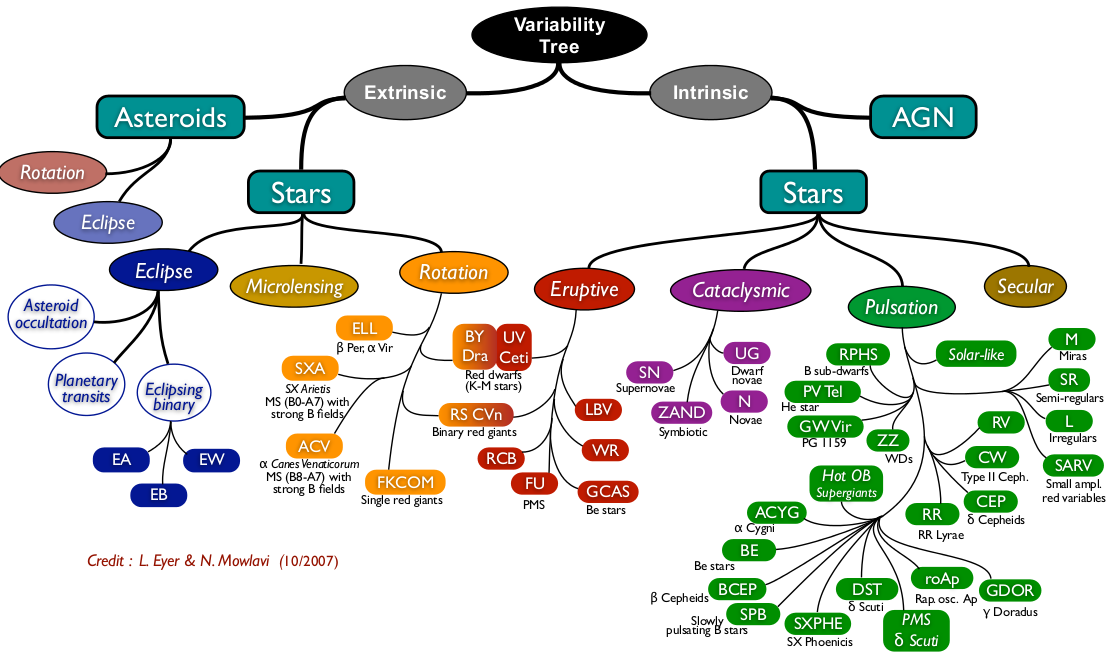
\includegraphics[height=0.78\linewidth,angle=-90]{Chapter1/variable_EyerMowlavi08.png}
    \caption[Variability classification tree]{Reproduction of \citet{eyer_variable_2008} classification tree of different variability types. Variable stars are the focus of this thesis so other variable objects at the second division level will not be discussed.}
    \label{fig:variability_tree}
\end{figure}

At the first division, intrinsic variables refer to stars where the variability is due to a physical process occurring withing the star itself. Extrinsic variability refers to cases where the geometry of the observations results in variability. This thesis is only concerned with variable stars and other variable object types will not be discussed, so the second division is not considered here. 

The third differentiation is based on the specific physical phenomenon at the object that causes the variability. The largest intrinsic category is stellar pulsations with almost all stars now known to exhibit this form of variability. Stellar rotation showing different regions of the surface, and eclipsed stars make up the most common examples of extrinsic variability. At the lowest level the different variable classifications are clustered together based on similar variability characteristics.

The classes are not all distinct at the lowest level, with some continuous transitions as the star passes from one evolutionary stage to another. To further complicate this process, variable stars may show signatures of more than one of these sources. (e.g. An eclipsing binary with a rotating red giant companion and a transiting exoplanet could show signatures belonging to four of these categories.) 

Detecting stellar variability at the lowest levels relies on accurate, and precise photometric measurements with continuous observations over long time periods.
There have been many missions and surveys over the past two decades dedicated to obtaining multi-epoch photometry including both ground-based missions (e.g. \textsc{Macho}, \textsc{Ogle} (I, II, and III), LSST, PanSTARRS, SONG, and HAT) and space-based telescopes (e.g. \Kepler, \Gaia, MOST, and \textsc{CoRoT}).

%Discussion & CRITIQUE of diagram. Bias etc
This figure was produced primarily for the classification of variables found in the \Gaia~mission and so is biased towards the broader classification of variable objects. Solar-like oscillators are combined into a single object classification in this schema, yet they account for a large proportion of the pulsating stellar variable population and are diverse in nature. This classification further separates stellar objects at different evolutionary stages into completely separate classifications. For example, evolved red giant stars showing Mira-like pulsations show no common branches with the solar-like oscillators they evolved from.

The introduction of photometric space-based telescopes to study solar-like stars (e.g MOST) and to search for exoplanets around them (e.g \Kepler, \textsc{CoRoT}, and TESS) have provided high precision photometry with the quality and quantity of data necessary to detect these oscillations unambiguously \citep{stello_detection_2010}. This data has revolutionised the study of stellar variability since the publication of the variability classification scheme above (e.g \citet{chaplin_asteroseismic_2010}  and \citet{basu_determination_2010}). 
\todo{CHECK THESE REFERENCES!!}



Importance of variable stars
    - Pulsating stars
        - Interior of stars (asteroseismology)
    - Eclipsing binaries
        - Masses of stars
    - Transits
        - Exoplanet hunting
    - Rotation
        - Splitting of modes
        - Spots
        - Magnetic field investigations

\subsection{Pulsating stars}

Pulsating variable stars are particularly important in expanding our understanding of stellar processes, interiors, and evolution. These stars are intrinsic variables; physical changes within the star are responsible for their variability. 

Different types of pulsating stars
Processes and Mechanisms - kappa, stochastic, convective blocking, tidal excitation
HR Diagram defined, show different variables and how they correspond to different regions.
Importance of variable stars
How we measure pulsations - asteroseimology.

Eddington - How can we see inside stars.
Asteroseismology. As such intrinsically variable stars are interesting
Almost all stars are intrinsically variable we have found as the detection limit is lowered.


% Pulsating variable stars are intrinsic variables as their variation in brightness is due to a physical change within the star. In the case of pulsating variables this is due to the periodic expansion and contraction of the surface layers of the stars. This means the star actually increases and decreases in size periodically. The different types of pulsating variable are distinguished by their periods of pulsation and the shapes of their light curves. These in turn are a function of the mass and evolutionary stage of a given star.

% The study of pulsating variables is of great importance to astronomers. Analysis of light curves provides vital information about the interior processes in stars. Perhaps their most valuable property of many types of pulsating variables is a direct relationship between the period of pulsation and their luminosity. This in turn allows us to determine the distance to such stars and is discussed in more detail on the next page.

% As with non-pulsating variables, there are several types of pulsating stars and some of the key types are described briefly below.


% We observe pulsational variability in stars of all types.  exhibit pulsational variations, driven by one of two oscillation mechanisms. % There are two main processes which excite stellar oscillations, the heat-engine mechanism
% (Eddington, 1926), and stochastic excitation (e.g. Unno, 1964). The heat-engine mecha-
% nism was first proposed by Eddington who considered pulsating stars as thermodynamic
% heat engines where radial oscillations result from sound waves resonating in the stellar
% interior. In this mechanism, a shell of stellar mass loses its support against the gravita-
% tional field of the star and collapses towards the centre of the star. This collapse results
% in the compression of the shell s mass which in turn restricts the radiation transfer from
% the stellar core and increases the shell s temperature. This temperature increase causes a
% respective increase in the pressure acting on the shell, forcing it to expand. As it expands,
% 1the radiation pressure decreases and the shell cools down forcing the shell to collapse once
% more.

% driving these  The Hertzsprung-Russel (HR) Diagram 

% HR Diagram is a tool that can be used to show the pulsating stars.

% Murphy Thesis
% The A stars exhibit a range of pulsation phenomena. This is where many of the
% classical pulsators—those driven by the ‘heat-engine’ mechanism—are found. Under
% this mechanism, first proposed by Eddington (1917), a layer heats up on compression,
% increasing the region’s opacity and driving radius expansion. The expanded region
% later cools, causing an opacity drop and re-compression. The dependence on opacity
% has lead to the mechanism being known as the opacity-, or simply κ-mechanism.
% The RR Lyrae variables, rapidly oscillating Ap (roAp) stars and δ Scuti stars are all
% examples of A stars driven by the κ-mechanism. Classical Cepheid variables are also
% driven by the κ-mechanism, but at later spectral types. The γ Doradus variables make
% up a large number of variables at early-F spectral types, but are driven by a convective-
% flux modulation mechanism (Guzik et al. 2000). Some stars show pulsations driven
% by more than one mechanism and are known as hybrids (Handler 2012).

% We will refer to pulsation modes using quantum numbers: n is the overtone or
% radial order of the mode, indicating the number of radial nodes; l is the degree, indi-
% cating the number of surface nodes; and m is the azimuthal order, with |m| indicating
% the number of surface nodes that are also lines of longitude. We shall see later that
% the sign of m indicates whether the mode is prograde or retrograde, and we use the
% convention that prograde modes have negative m values and higher frequencies in the
% observer’s frame. Pressure modes (p modes) are denoted with positive values of n,
% and gravity modes (g modes) with negative values. One sometimes writes p 1 , p 2 ,...,
% to denote the n-value of the p modes. The g modes are always non-radial, that is, they
% have l ≥ 1. Spherically symmetric stars have degenerate pulsation frequencies, in
% that all modes with the same (n, l) have the same frequency, regardless of m. Rotation
% and magnetic fields can break the symmetry and lift this degeneracy, however.

% Jason Thesis
% 1.1.1 Oscillation Mechanisms
% There are two main processes which excite stellar oscillations, the heat-engine mechanism
% (Eddington, 1926), and stochastic excitation (e.g. Unno, 1964). The heat-engine mecha-
% nism was first proposed by Eddington who considered pulsating stars as thermodynamic
% heat engines where radial oscillations result from sound waves resonating in the stellar
% interior. In this mechanism, a shell of stellar mass loses its support against the gravita-
% tional field of the star and collapses towards the centre of the star. This collapse results
% in the compression of the shell s mass which in turn restricts the radiation transfer from
% the stellar core and increases the shell s temperature. This temperature increase causes a
% respective increase in the pressure acting on the shell, forcing it to expand. As it expands,
% 1the radiation pressure decreases and the shell cools down forcing the shell to collapse once
% more.
% The κ mechanism (Eddington, 1941) is a heat-engine mechanism predominantly ob-
% served in classical pulsators such as RR-Lyrae, δ-Scuti and Cepheid stars which results
% from changes in opacity within the star. Ionisation of helium and hydrogen within the
% stellar envelope, resulting from the absorption of radiation from nuclear fusion, produces
% regions of higher relative opacity than the surrounding non-ionised layers. These zones of
% higher opacity store flux from the inner layers when compressed (Zhevakin, 1958). This
% energy absorption causes the layers to expand towards their equilibrium point, resulting
% in the release of the temporarily-stored energy. The layer however continues expanding
% beyond its equilibrium position as it cools decreasing its opacity and allowing more flux
% to escape, inducing oscillations around the equilibrium (King and Cox, 1968).
% Variable stars which exhibit solar-like oscillations such as red giants, cool sub-giants
% and lower main sequence stars are characterised by stochastically excited oscillations.
% These randomly-excited oscillations evolve from turbulence within a thick, convective
% layer in the outer envelope of the star. The turbulent driving force for these oscillations
% occurs in the region of this convective layer where the time scales for the pulsations and
% convection are closely correlated (Handler, 2013). For such a convective layer to form,
% the stars must be cooler than the red edge of the classical instability strip where classical
% pulsators reside (Bedding, 2011), see Figure 1.1.
% The turbulence within these variable stars perturbs the stellar structure, forming nor-
% mal modes and thus global oscillations when they coincide with standing wave frequencies.
% Despite constant convective forcing, these modes have a finite lifetime resulting from de-
% structive interference with out-of-phase stochastic excitations. Any oscillations which do
% not correspond to normal modes decay rapidly due to internal damping and are not ob-
% served as global oscillations. Such solar-like oscillators shall be the main topic of this
% research project.
% Photometry is one analytical technique utilised for detecting and investigating stellar
% oscillations and relies upon on the detection of variations within the stellar luminosity
% measurements to detect source variability. Stellar luminosity is affected by a combination
% of both the temperature and radius of the star. The particular characteristic which
% dominates this interaction depends on the specific wavelength regime and the type of star
% being considered. For red giant stars for instance, changes in the stellar radius tend to
% dominate this relation.

% ----

\begin{figure}[htbp]
    \centering
    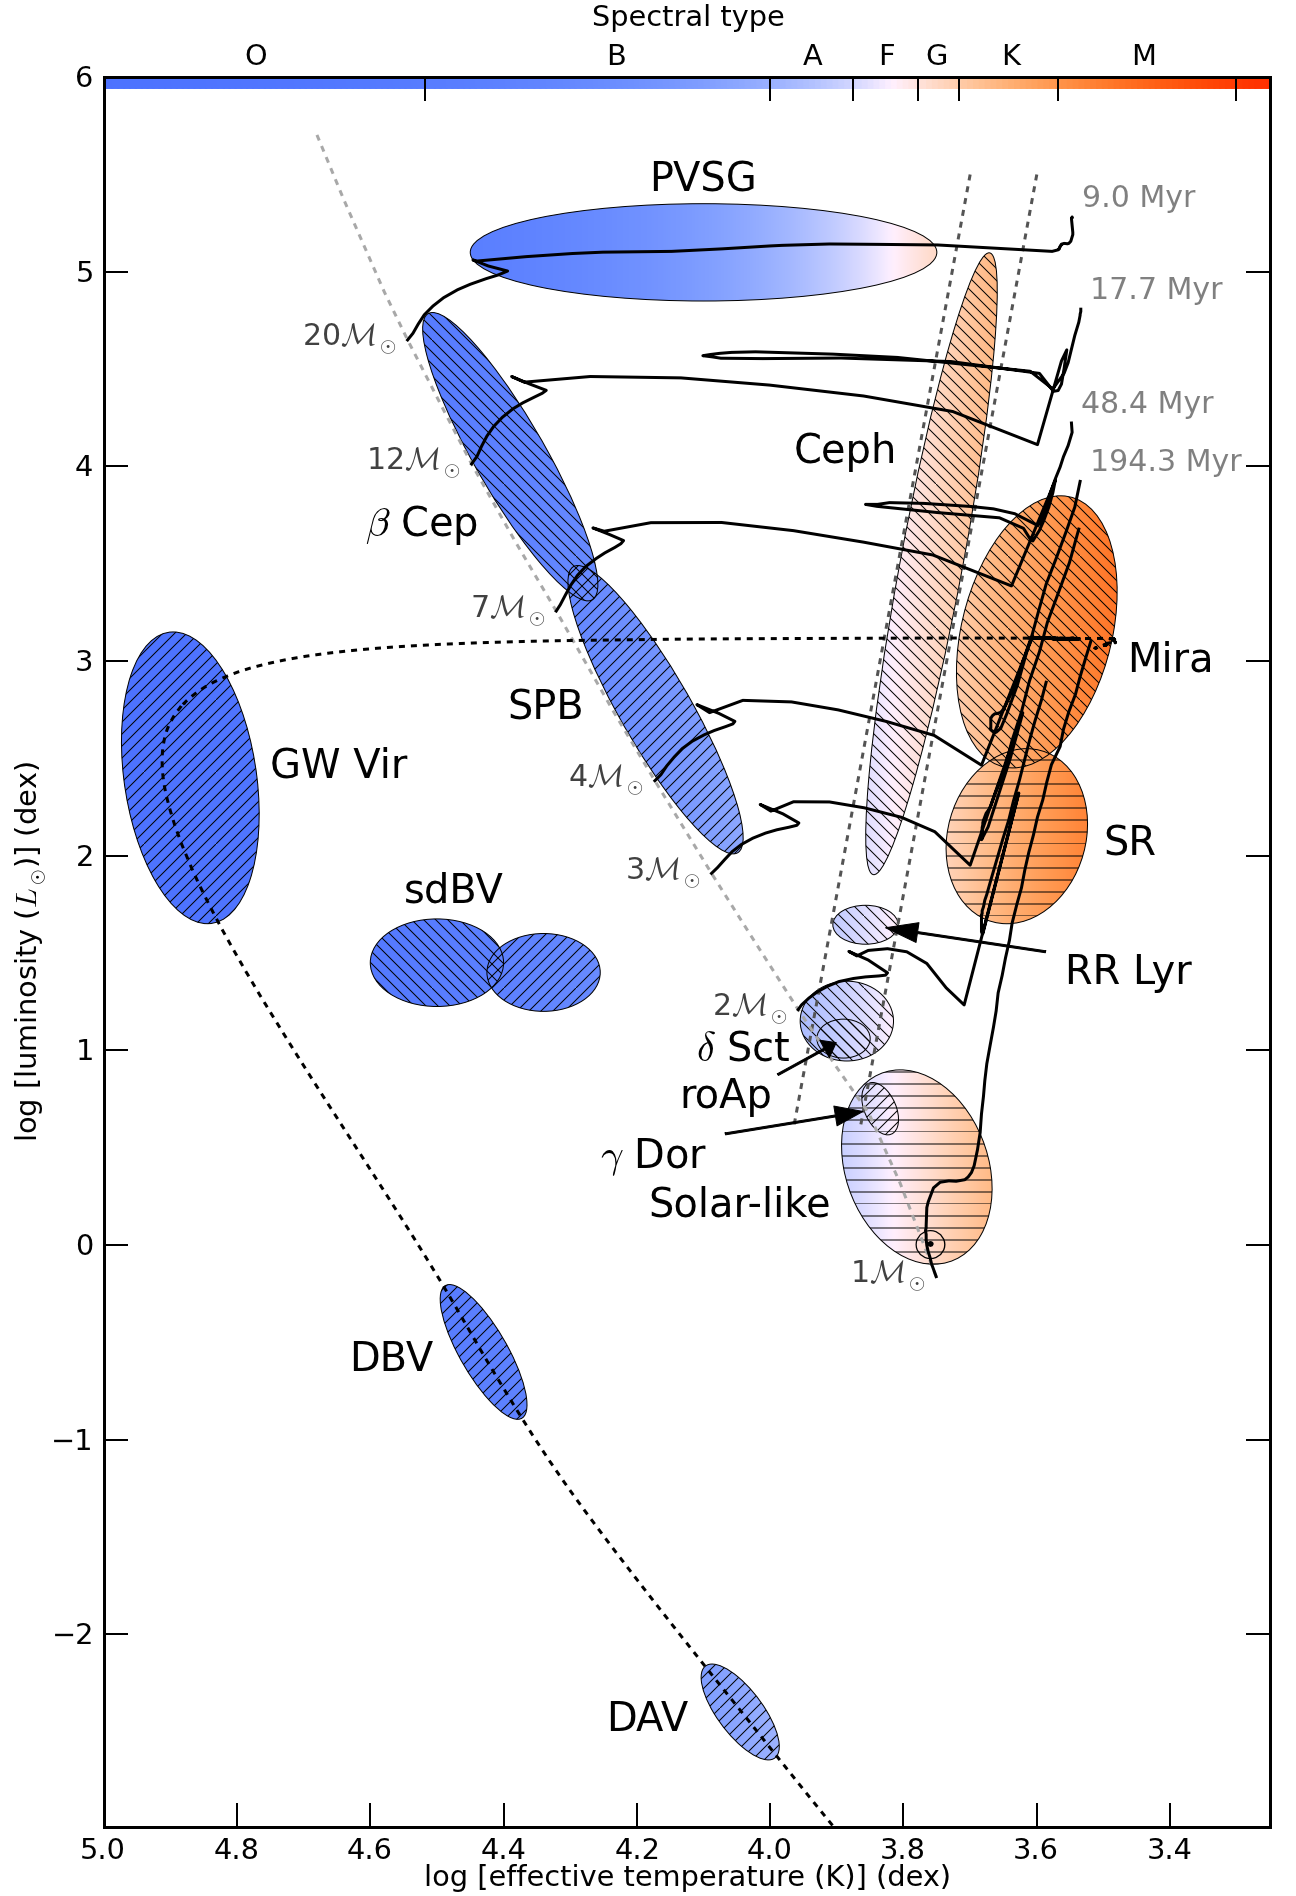
\includegraphics[height=0.5\paperheight]{Chapter1/HR_pulsational.png}
    \caption[Pulsational Hertzsprung-Russell Diagram]{}
    \label{fig:HRdiag}
\end{figure}

HR diagram showing variable star regions - P. Begroote, P. Papics

Oscillation mechanisms

% Excitation mechanisms
%\kappa -mechanism
% Main article: Kappa mechanism
% Under fairly specific conditions, some stars have regions where heat is transported by radiation and the opacity is a sharply decreasing function of temperature. This opacity bump can drive oscillations through the {\displaystyle \kappa } \kappa -mechanism (or Eddington valve). Suppose that, at the beginning of an oscillation cycle, the stellar envelope has contracted. By expanding and cooling slightly, the layer in the opacity bump becomes more opaque, absorbs more radiation, and heats up. This heating causes expansion, further cooling and the layer becomes even more opaque. This continues until the material opacity stops increasing so rapidly, at which point the radiation trapped in the layer can escape. The star contracts and the cycle prepares to commence again. In this sense, the opacity acts like a valve that traps heat in the star's envelope.

% Pulsations driven by the {\displaystyle \kappa } \kappa -mechanism are coherent and have relatively large amplitudes. It drives the pulsations in many of the longest-known variable stars, including the Cepheid and RR Lyrae variables.

% Surface convection
% In stars with surface convection zones, turbulent fluids motions near the surface simultaneously excite and damp oscillations across a broad range of frequency.[2][3] Because the modes are intrinsically stable, they have low amplitudes and are relatively short-lived. This is the driving mechanism in all solar-like oscillators.

% Convective blocking
% If the base of a surface convection zone is sharp and the convective timescales slower than the pulsation timescales, the convective flows react too slowly perturbations[clarification needed] that can build up into large, coherent pulsations. This mechanism is known as convective blocking[4] and is believed to drive pulsations in the {\displaystyle \gamma } \gamma  Doradus variables.[5]

% Tidal excitation
% Observations from the Kepler satellite revealed eccentric binary systems in which oscillations are excited during the closest approach.[6] These systems are known as heartbeat stars because of the characteristic shape of the light curves.





Variable stars in open clusters


%----------------------------------------------------------------------------------------------------------------------------------------------------------------
%----------------------------------------------------------------------------------------------------------------------------------------------------------------


\section{Open clusters}

Open clusters are typically characterised as sparse, loosely gravitationally-bound stellar populations located primarily in the galactic disk \citep{friel_old_1995}. Older open clusters tend to be more densely populated, with hundreds to thousands of members, compared to younger clusters that comprise a few tens to hundreds of members. These older open clusters also tend to be located at greater distances from the galactic disc, where the probability of collisions with large molecular clouds, that disperse cluster members among the galactic field population, are more remote \citep{}. \todo{Get reference from pad on bookshelf/in paper box?} Tidal disruption, disc and bulge shocking, and stripping from galactic field interactions are also responsible for the dissolution of stellar cluster members into the field population \citep{marchi_search_2006}. All of these processes are most prevalent in the galactic disc.\todo{Check this statement}

Stellar cluster populations form within a single nebula and consist of coeval, isometallic, cospatial and comoving members \citep{baade_resolution_1944}, with initial stellar mass being the primary parameter that differentiates members. \citet{mould_stellar_1982} showed that the metallicity and kinematics of cluster members are unchanged by stellar and galactic evolution, making cluster members ideal probes for a wide range of astrophysical investigations (e.g stellar interiors and atmospheres \citep{}, stellar evolution \citep{kalirai_jason_s._star_2010}, cosmology \citep{}, galactic evolution \citep{de_grijs_revolution_2010}, and disk and planet formation \citep{}).

In terms of stellar evolutionary studies, the fewer free parameters required for modelling cluster members allows the analysis to be conducted as a uniform ensemble, with a few exceptions resulting from rotation, magnetic field interactions and binarity \citep{carroll_introduction_2006}. Whilst globular clusters may experience multiple stellar formation epochs, this is not the case for open clusters \citep{li_stellar_2016} that are instead well-described by a single isochrone (a composite of coeval theoretical evolutionary tracks for different initial mass values) transformed to the observational CMD regime. Photometric observations of cluster members reveal outliers from these isochrones, with binarity being perhaps the most influential cause (e.g. \citet{duquennoy_multiplicity_1991} and \citet{murphy_finding_2018}), resulting in apparent magnitudes of up to 0.75\,mag brighter for unresolved binaries.

This thesis will focus on the four open clusters located in the nominal \Kepler field of view; NGC\,6791, NGC\,6819, NGC\,6811, and NGC\,6866. These clusters span a range of ages and metallicities. Table \ref{tab:cluster_properties} presents a summary of the global cluster properties.

\subsection{NGC 6791}

From Honours: 
NGC 6791 is an open cluster located in the Lyra constellation at a distance of approximately 4.1\,kpc \citep{basu_determination_2010}. It is one of the oldest, most metal-rich open clusters with an approximate age of 8 Gyrs (\citet{grundahl_2008}, \citet{king2005}, \citet{stetson_2003}) and metallicity [Fe/H] = +0.30 \citep{boesgaard_2009}. The high metallicity of this cluster is atypical, as older stellar clusters tend to have lower metallicities than younger ones, originating from the initial chemical composition of the dust cloud they form from. The population density of cluster members is also much higher than most other open clusters and combined with its metal-rich nature has led to NGC 6791 becoming one of the most studied open clusters in the galaxy. Previous studies of this cluster have reported age discrepancies/discontinuities between cluster members with the faint white dwarf members having much younger ages of approximately 4 to 6 Gyrs compared to the average of 8 Gyrs for the majority of the cluster members \citep{Bedin2008}. Theoretical investigations however revised the calculations for white dwarf age determination and demonstrated a common age of 8 Gyrs for all cluster members investigated \citep{Garciaberro2010}. 

\subsection{NGC 6819}

NGC 6819 is an open cluster located approximately 2.16 kpc away in the Cygnus constellation (Balona et al., 2013). It is a much younger open cluster than NGC 6791 with an average stellar age of approximately 2.5 Gyrs (Kalirai et al., 2001; Rosvick and Vandenberg, 1998) and solar metallicity of [Fe/H] = +0.09 (Bragaglia et al., 2001).


\subsection{NGC 6811}
\subsection{NGC 6866}

% There are four open clusters spanning a range of ages and metallicities within the
% Kepler field of view (FOV); NGC 6791, NGC 6811, NGC 6866 and NGC 6819. Several
% membership and quantitative studies have already been conducted on these clusters based
% solely on observations of stars targeted for observation and analysis by the Kepler mission
% (Basu et al., 2011). The first clear measurements of solar-like oscillations in these cluster
% stars were detected through relative flux variations and presented by Stello et al. (2010).

% NGC 6791 is an open cluster located in the Lyra constellation at a distance of approxi-
% mately 4.1 kpc (Basu et al., 2011). It is one of the oldest, most metal-rich open clusters
% with an approximate age of 8 Gyrs (Grundahl et al., 2008; King et al., 2005; Stetson et al.,
% 2003) and metallicity [Fe/H] = +0.30 (Boesgaard et al., 2009). The high metallicity of this
% cluster is atypical, as older stellar clusters tend to have lower metallicities than younger
% ones, originating from the initial chemical composition of the dust cloud they form from.
% The population density of cluster members is also much higher than most other open
% clusters and combined with its metal-rich nature has led to NGC 6791 becoming one
% of the most studied open clusters in the galaxy. Previous studies of this cluster have
% reported age discrepancies/discontinuities between cluster members with the faint white
% dwarf members having much younger ages of approximately 4 to 6 Gyrs compared to the
% average of 8 Gyrs for the majority of the cluster members.(Bedin et al., 2008) Theoretical
% investigations however revised the calculations for white dwarf age determination and
% demonstrated a common age of 8 Gyrs for all cluster members investigated.(Garcı́a-Berro
% et al., 2010)

% NGC 6819 is an open cluster located approximately 2.16 kpc away in the Cygnus constel-
% lation (Balona et al., 2013). It is a much younger open cluster than NGC 6791 with an
% average stellar age of approximately 2.5 Gyrs (Kalirai et al., 2001; Rosvick and Vanden-
% berg, 1998) and solar metallicity of [Fe/H] = +0.09 (Bragaglia et al., 2001).
\begin{table}[h]
    \setlength\tabcolsep{10pt}
    \centering
    \begin{tabular}{lcccc}
        \hline
                        & NGC 6791 & NGC 6819 & NGC 6811 & NGC 6866 \\
        \hline
        \hline
        RA                      &  &  &  & \\
        Dec                     &  &  &  & \\
        Distance                &  &  &  & \\
        Age (Gyrs)              &  &  &  & \\
        Metallicity [Fe/H]      &  &  &  & \\
        Radius                  &  &  &  & \\
         - Core                 &  &  &  & \\
         - Tidal                &  &  &  & \\
         - Limiting             &  &  &  & \\
         Population             &  &  &  & \\
        \hline
        
    \end{tabular}
    \caption{A summary of the global properties of the four open clusters in the nominal \Kepler field of view; NGC\,6791, NGC\,6819, NGC\,6811, and NGC\,6866.}
    \label{tab:cluster_properties}
\end{table}


%----------------------------------------------------------------------------------------------------------------------------------------------------------------
%----------------------------------------------------------------------------------------------------------------------------------------------------------------

\section{Kepler}
NASA's \Kepler~space telescope was a 1.4m modified Schmidt design that completed its nominal mission between May 2009 and May 2013. It was designed primarily to detect transiting exoplanets by obtaining micro-magnitude precision photometry of approximately 150\,000 stars within its field of view. The ultimate goal was the detection of Earth-sized exoplanets in the habitable zone of solar-like stars, and the determination of the populations of such planets in the Milky Way \citep{koch_kepler_2010}.

Figure \ref{fig:KepSchema} shows a schematic diagram of the \Kepler~space telescope components; the photometer, made up of the telescope and detector, and the spacecraft itself.  The telescope included a 1.4\,m primary mirror and a 0.95\,m aperture Schmidt corrector plate focusing light onto a 95 megapixel detector at the focal plane. The spacecraft included a solar array, thermal radiator, a high-gain (Ka-band) antenna for data transmission, four reactor wheels, and thruster modules.

\begin{figure}[htbp]
    \centering
    \vspace{0.5em}
    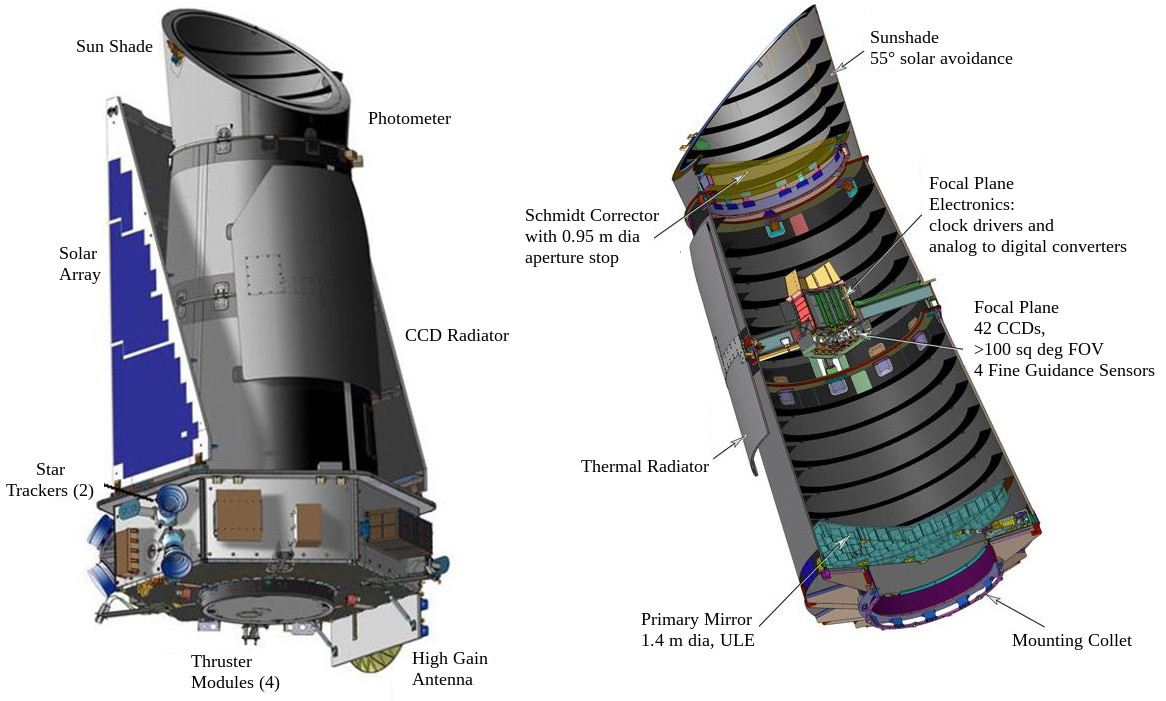
\includegraphics[width=0.9\linewidth]{Chapter1/Kepler_schema_both.jpg}
    \vspace{0.5em}
    \caption[Schema of the \Kepler~spacecraft]{Schema of the \Kepler~space telescope showing (a) The main components of the spacecraft and (b) A cutout of the photometer highlighting the internal structure including the focal plane, 1.4\,m primary, 0.95\,m schmidt corrector plate, and the positioning of the CCD detector.}
    \label{fig:KepSchema}
\end{figure}

The detector (Figure \ref{fig:Kep_detect}) was composed of 42 thinned, back-illuminated CCDs of dimensions 50\,mm $\times$ 25\,mm, arranged into 21 square modules. Each CCD had a resolution of 2200 $\times$ 1024 pixels (px) with a physical pixel size of 27 $\mu m^2$. This detector was maintained at -85\,$\degree$C via the thermal radiator to ensure near constant efficiency of the CCDs.

\begin{figure}[htbp]
    \centering
    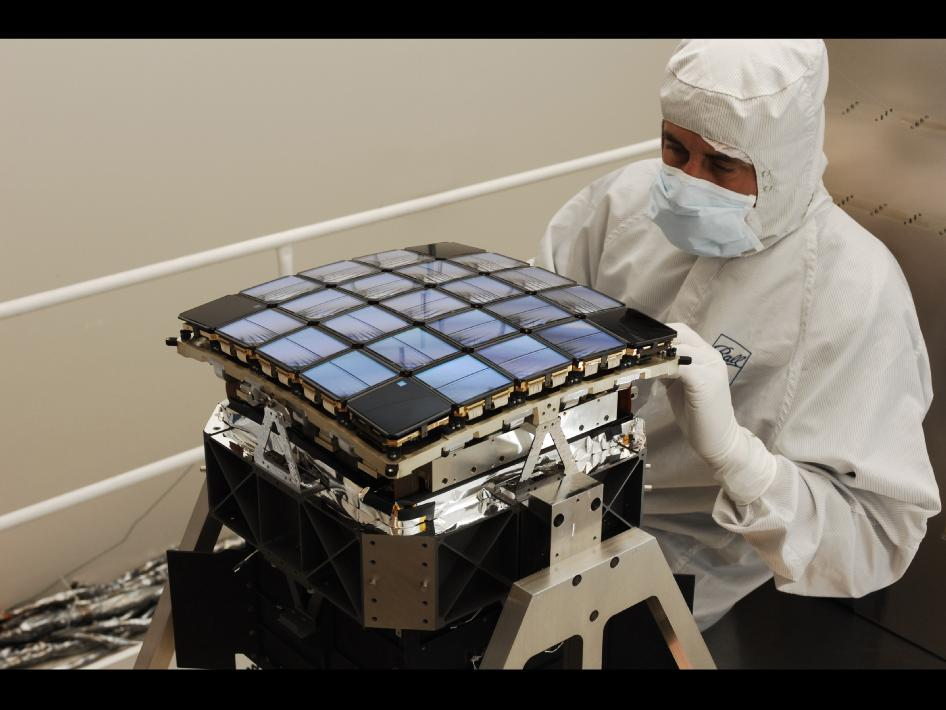
\includegraphics[width=0.45\linewidth]{Chapter1/Kepler_detector.jpg}
    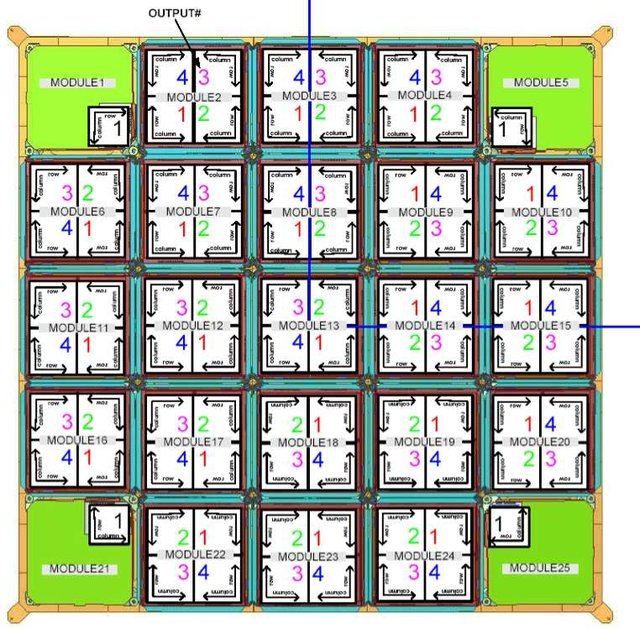
\includegraphics[width=0.45\linewidth]{Chapter1/kepCCD.jpg}
    \caption[Kepler CCD detector array prior to installation]{Left: The focal plane array assembly showing the 42 CCDs that comprised the detector at Bell Labs prior to launch. Right: A schematic of the detector module placements and identification of each module and output. Module positions 1, 5, 21, and 25 are occupied with fine guidance sensor chips.}
    \label{fig:Kep_detect}
\end{figure}

\subsection{Mission}
For the nominal mission \Kepler~maintained a 105 square degree field of view (FoV) centred between the constellations of Cygnus and Lyra, and located 13.5 degrees above the galactic plane. Figure \ref{fig:kepFoV} presents a stylised representation of the telescope's nominal FoV with stellar magnitudes represented by the size of the filled circles. The four open clusters that are present are marked by dashed lines. Note that the detector is positioned to ensure the brightest stars are focussed between the modules to minimise blooming (overexposure and charge-bleeding along CCD rows). This FoV produces a pixel scale of 3.98\,"/px. The telescope was intentionally defocussed to diffuse the light of a stellar target to 10\," to ensure the best possible photometric stability.

\begin{figure}[htbp]
    \centering
    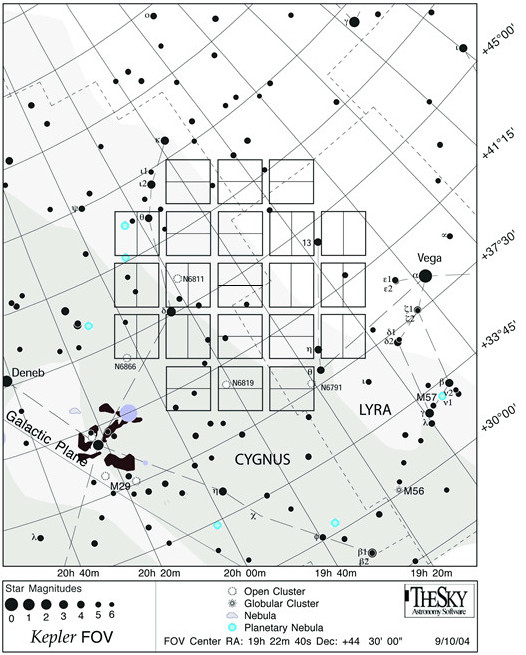
\includegraphics[height=0.32\paperheight]{Chapter1/kepFoV.jpg}
    \vspace{0.5em}
    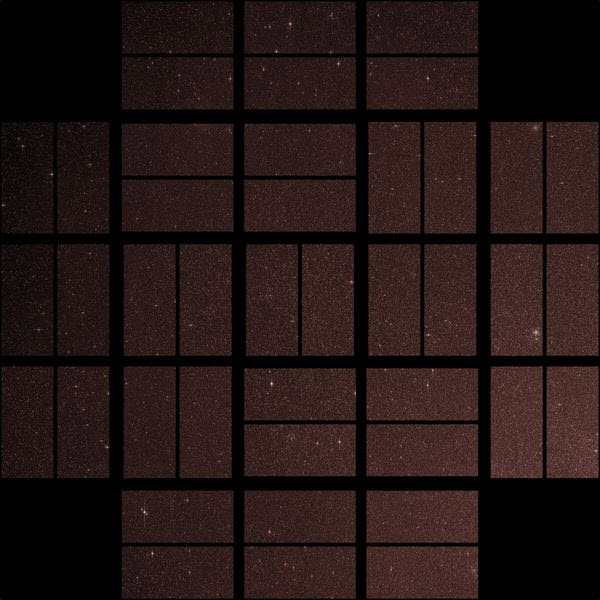
\includegraphics[width=0.45\linewidth]{Chapter1/kepFFI.jpg}
    \caption[\Kepler field of view; stylised, and full-frame image]{Left: Stylised representation of the \Kepler\, field of view between the constellations of Cygnus and Lyra. Larger filled circles represent stars of brighter magnitude. The four open clusters in the FoV are designated by dashed circles. Right: An example of the full-frame images (FFIs) of \Keplers~FoV.}
    \label{fig:kepFoV}
\end{figure}

\Kepler~occupied an Earth-trailing heliocentric orbit (ETHO) with the field of view selected to avoid Earth-shine, Moon-shine, and sunlight from entering the photometer. One of the characteristics of an ETHO are lower torques acting on the spacecraft, enabling more efficient fine-pointing control. This control is achieved through the four reactor wheels that spin up to store the angular momentum from the acting torques before being dumped through thruster burns. The orbit also required the spacecraft to rotate every 90\,days to maintain sunlight on the solar array and exposure of the thermal radiator to deep space, placing stars on different CCDs. This rotation resulted in data being divided into "quarters" at each rotation. The initial 30\,d observing run following the 10\,d engineering test but prior to the first rotation is termed quarter 1 (Q1), with the nominal mission terminating after Q17 due to the failure of a second reaction wheel. These observations provide baseline photometry for most target stars of approximately 1\,460\,days.

\subsection{Data Products}

Whilst the ETH orbit is much more fuel efficient than an Earth-centric one, the constantly increasing distance between the spacecraft and Earth limits the bandwidth available for data down-link through NASA's Deep Space Network. Full-frame images (FFIs) of \Keplers~FoV were too large to be downloaded at the cadence required for the mission's science goals, so subsets of these images were selected for down-link, with a single FFI (Figure \ref{fig:kepFoV}) downloaded every 30\,d \citep{thompson_kepler_2016}. All data products from the mission preserved pixel-level data, so subsets could be queried per pixel. Module 3 of the CCD detector failed in January 2010, so all stars that fell on this module have data gaps every four quarters that correspond to the spacecraft's rotation.

\subsubsection{Target Pixel Files}
The primary data products consisted of subsets or `postage stamps' of the CCD array output around target stars called target pixel files (TPFs) and were produced for around 150\,000 targeted stars per quarter. There were two observational cadences for the TPFs; long cadence (LC) observations with a total exposure time of 29.43\,m, and a smaller subset of approximately 500 short cadence (SC) observations with an exposure time of 58.86\,s. The LC exposures consisted of 270 CCD readout cycles (6.02\,s exposure followed by 0.52\,s readout per cycle) co-added on board the spacecraft while the SC TPFs consisted of 9 co-added cycles. These were stored in on-board memory until down-link, every 30\,days.

\subsubsection{Superstamp Images}
In addition to the primary data products, large 200 $\times$ 200\,px `superstamps', centred on the open clusters of NGC\,6791 and NGC\,6819, were downloaded at LC exposure intervals for quarters 1 to 17. Figure \ref{fig:SS} shows a typical exposure of these superstamp images for each cluster. NGC\,6819 fell on module 3 of the detector from Q2, so no superstamps are available for this cluster for Q6, Q10 or Q14.

\begin{figure}[htbp]
    \centering
    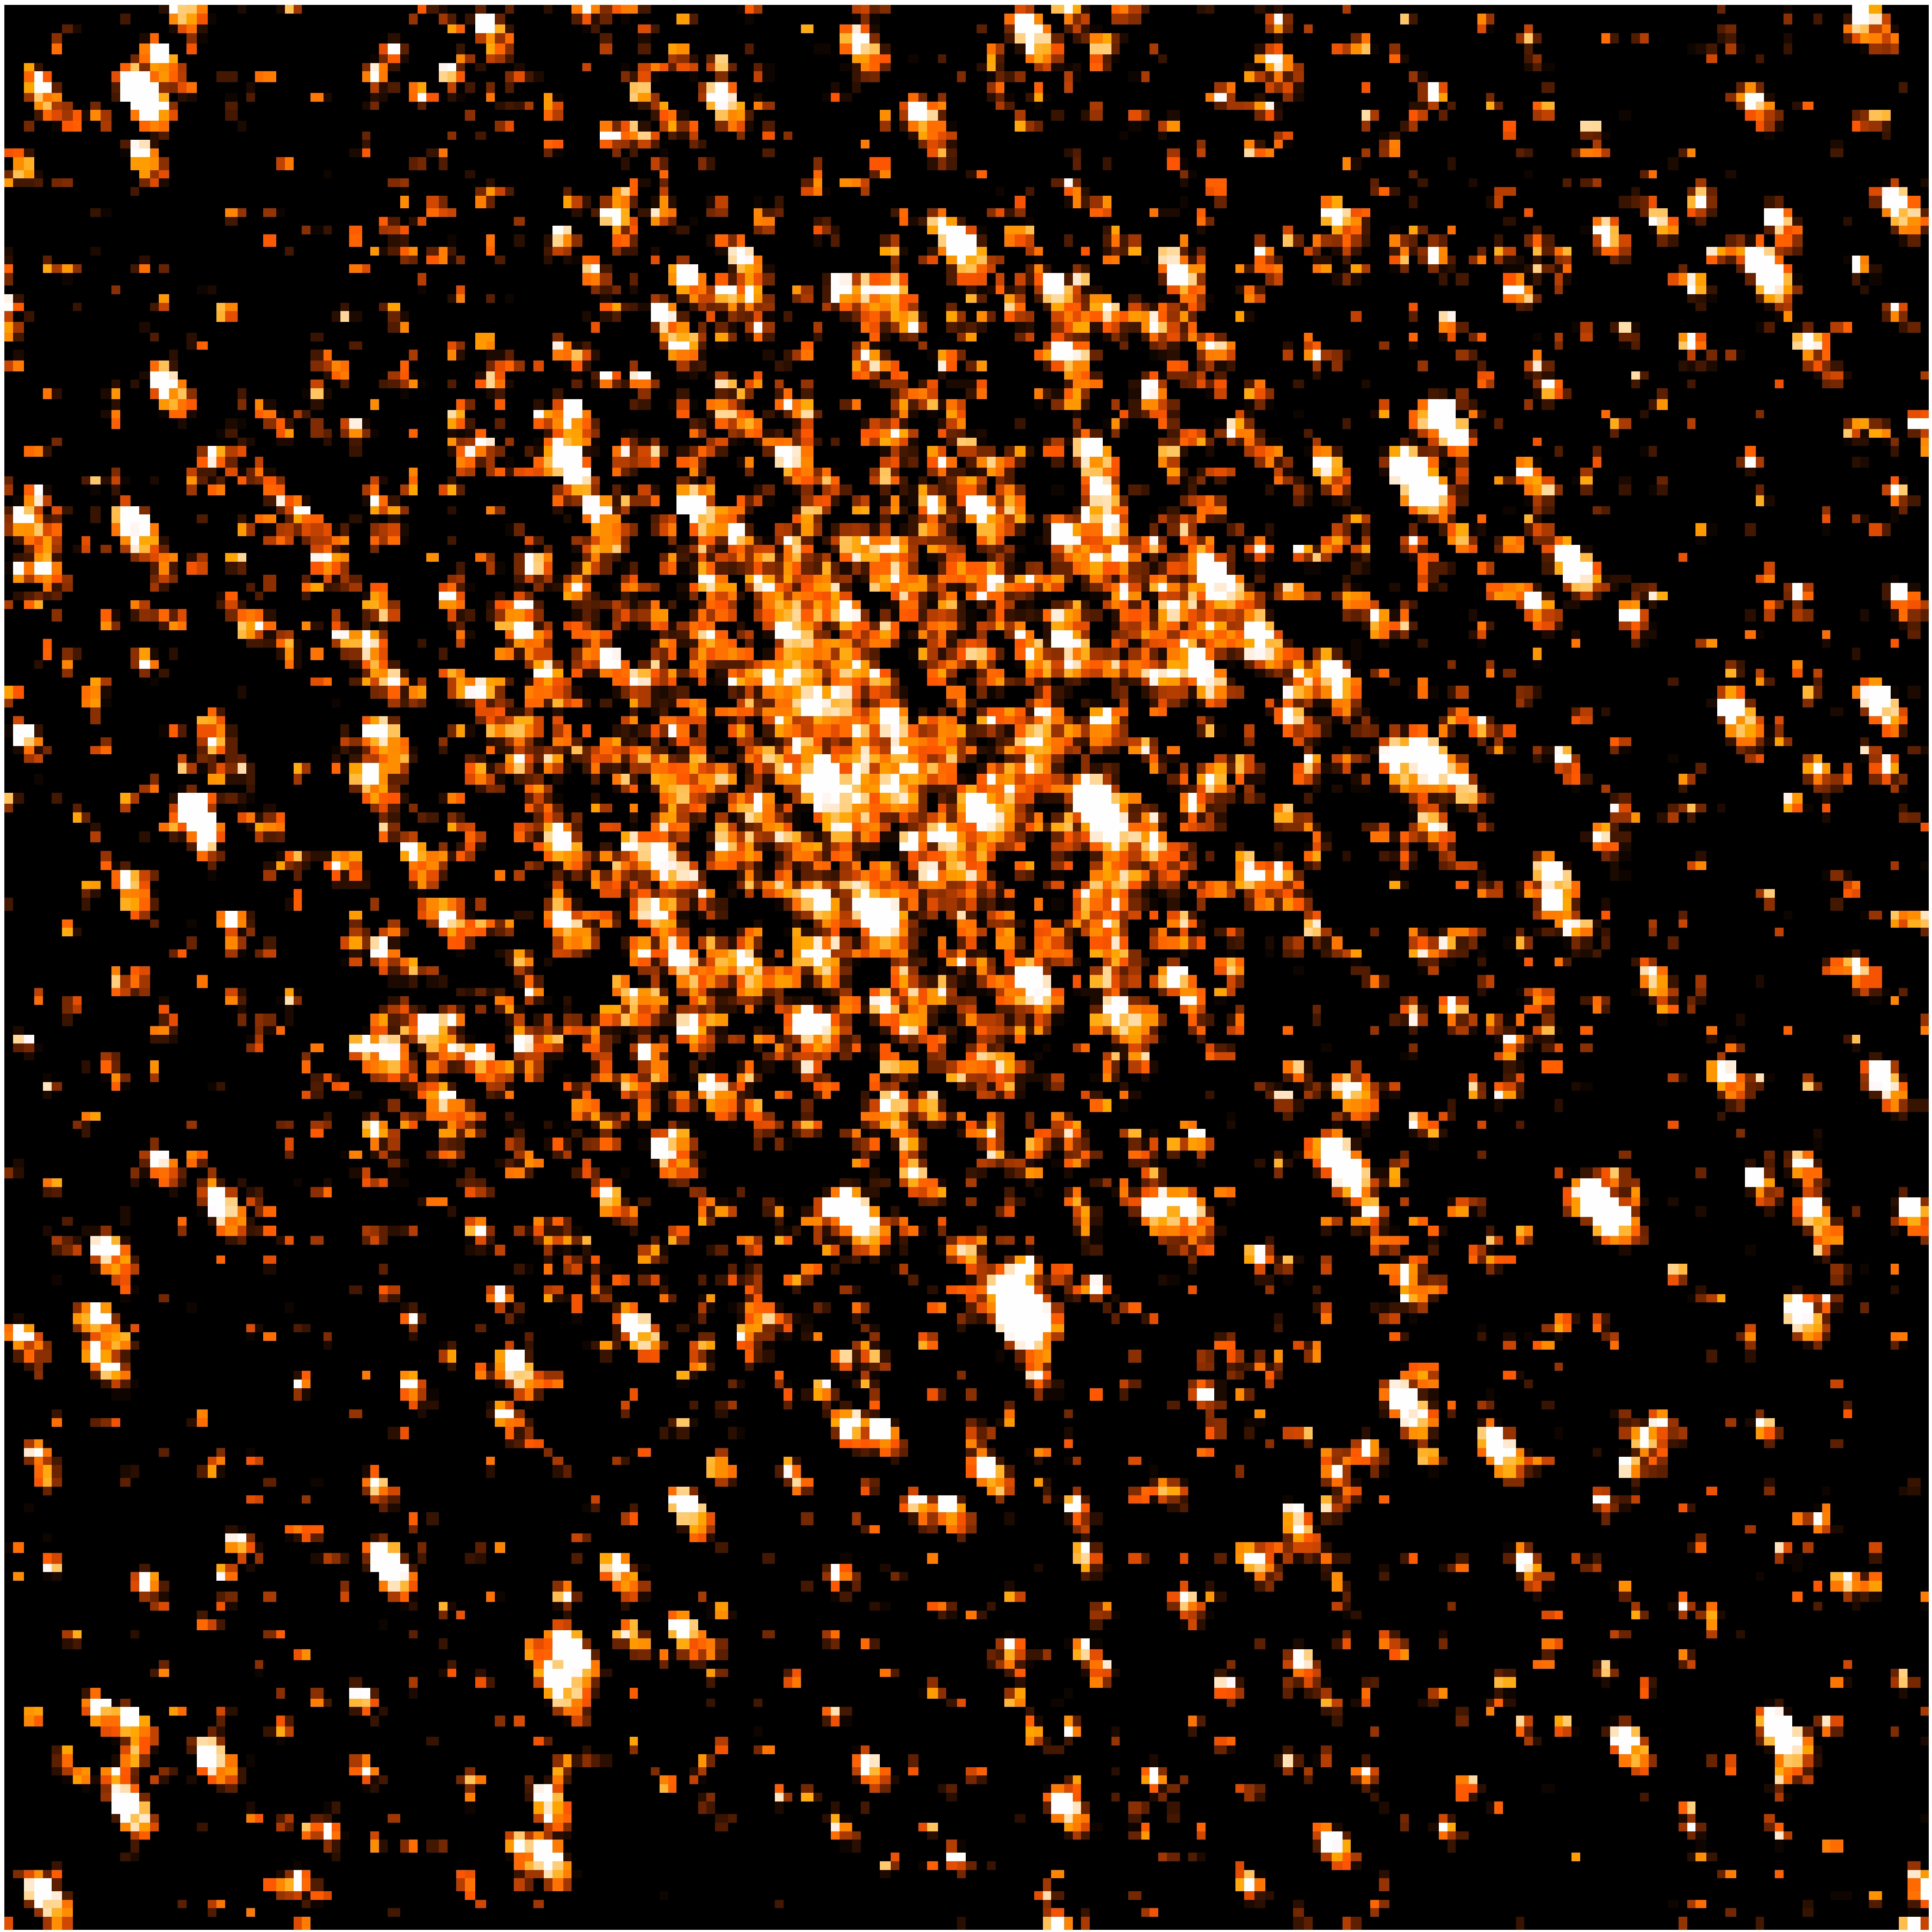
\includegraphics[width=0.45\linewidth]{Chapter1/ngc6791.jpg}
    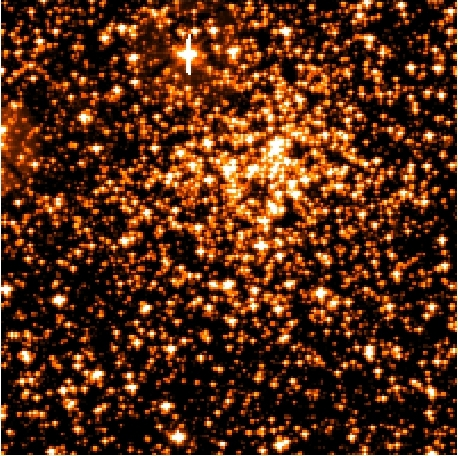
\includegraphics[width=0.45\linewidth]{Chapter1/ngc6819.jpeg}
    \caption[Superstamps of NGC\,6791 and NGC\,6819]{Typical exposures for superstamp images of the cores of the open clusters NGC\,6791 (left) and NGC\,6819 (right).}
    \label{fig:SS}
\end{figure}



%From honours thesis:
%"long, well-sampled time series with high accuracy in the measurements, are also critical for asteroseismic studies."
 




% Murphy Thesis
% Asteroseismology is the most informative method with which we can observe the
% stellar interior. Other than solar neutrinos, it is the only method. Oscillation fre-
% quencies present in stars’ light curves are the fundamental data of asteroseismology,
% and permit us to fine-tune stellar models. Although ground-based support is still
% required, particularly in constraining stellar atmospheric parameters and for direct
% mode identification, the existence of nearly continuous, micromagnitude-precision,
% space-based photometry is revolutionising our capacity to study stars.


%----------------------------------------------------------------------------------------------------------------------------------------------------------------
%----------------------------------------------------------------------------------------------------------------------------------------------------------------


\section{Photometric methods}



% Techniques for studying
% > CCDs - Simple ap phot
%       - PS phot
%       - Image sub

\subsection{Simple aperture photometry (SAP)}

\subsection{Point spread function (PSF) photometry}
Also known sometimes as pixel response function (PRF) photometry.

\subsection{Image Subtraction} %Literature review - Photometry of variable stars and open clusters
\chapter{\Kepler Photometry of Field and Cluster stars}

\section{Initial work}
\subsection{Image subtraction}
Talk about DIAPL failure and Custom attempt.

\subsection{Simple box aperture photometry}
Did produce some simple box aperture photometric results that are comparable to the MAST photometry, albeit with a reduction in the S/N of approximately $\sqrt2$ in the power of the oscillations in the lightcurves.

Comparison of RG's PS to MAST

Number of LCs? ~1200

Interesting stars
- RR Lyrae
- EB's
- Transits> %Kepler and Open clusters - Initial SAP
\chapter{Rotational modulation in KIC\,2569073 an Ap star}

\section*{abstract}
    In this chapter we analyse KIC\,2569073\footnote[2]{Within the asteroseismology community there is a tradition of nicknaming stars with interesting light curves after pets. KIC\,2569073 is thus nicknamed Fluffy.}, an individual, non-targeted \Kepler superstamp star. It was initially considered to be a possible Cepheid variable star based on its photometric light curve. This would make it only the second known Cepheid in the nominal \Kepler field of view. We conclude however, that this is a non-oscillating Ap (noAp) star exhibiting rotational modulation, based upon multi-colour photometry and spectroscopic observations that eliminate the possibility of Cepheid classification.
    % \bigskip
\newpage
\section{Investigation of KIC\,2569073}

%We begin by providing a short introduction to Cepheid and A type stars that were the focus of this research and present additional details of the investigation prior to the paper itself.

During the initial SAP investigation of the \Kepler superstamps discussed in the previous chapter we discovered a particularly interesting light curve for KIC\,2569073. The light curve, extracted using a custom aperture derived for each quarter, showed an almost-sinusoidal variability reminiscent of classical Cepheid variable stars. 

Classical Cepheids are luminous giant and supergiant stars of spectral types F6-K2 \citep{rodgers_radius_1957} corresponding to stellar masses between 4\,\Msol~and 20\,\Msol~\citep{turner_progenitors_1996}. %The $\kappa$ mechanism acts within the helium ionisation zone of these stars to produce radial pulsations in these stars \citep{Eddington17}. These pulsations cause 
Cepheids show precise period variations in luminosity due to radial pulsations produced by the $\kappa$-mechanism acting in the helium ionisation zone \citep{eddington_pulsation_1917}. \citet{leavitt_1777_1908} discovered the period-luminosity relation for these stars leading to their use for galactic and extra-galactic distance determinations, and allowing for the later determination of the Hubble constant \citep{freedman_final_2001}. This relation relies on an accurate knowledge of a Cepheid's period. \citet{derekas_period_2012} detected period jitter in V1154 Cyg, the single Cepheid in the nominal \Kepler~FoV, with a random variation of the period on order 30\,mins over the 4.9\,d cycle. \citet{neilson_period_2016} produced simulations suggesting convective granulation could account for these observations. \citet{derekas_kepler_2017} analysis of the complete four year \Kepler~light curve confirmed the presence of granulation, and showed a possible connection between convection and the observed pulsation. Having a second Cepheid with \Kepler~data would help confirm this connection. 

Our analysis of the light curve, as described in the paper below, was almost complete prior to obtaining multi-colour photometry to check the preliminary Cepheid classification. Anti-phase variations between the B light curve and the $V$, $R_C$, and $I_C$ light curves however, contradicted this classification. This phenomenon is not characteristic of Cepheids but has been observed in $\alpha^2\,$CVn variable stars \citep{kurtz_determination_1996}, a type of chemically peculiar A-type (Ap) star. 

% Define Ap stars - chemically peculiar (1st discovered?)
% Why/how chemically peculiar?
% General characteristics:
%     How common?
%     roAp vs noAp (Kurtz et al.)
%         Oscillation mechanism
%         Known examples
%     Spots $\&$ mag fields
%         How generated?
%         Observations - effect on photometry?
%     Rotational modulation

Spectral A-type stars are main sequence stars with effective temperatures between approximately 7\,150\,K and 10\,150\,K \citep{murphy_kepler_2012}, corresponding to zero age main sequence (ZAMS) masses ranging between 1.4\,\Msol~ and 2.4\,\Msol. These stars don't necessarily remain as A-type stars for the duration of their main sequence lifetime, rather they tend towards cooler effective temperatures and thus spectral types as they evolve towards the terminal age main sequence (TAMS). Investigations of A-type stars between the ZAMS and TAMS must therefore include initial masses higher than 2.4\,\Msol. Fig. \ref{fig:Astar_evol_tracks}, reproduced from \citet{murphy_examination_2012}, shows evolutionary tracks for 1.7\,\Msol~to 3.5\,\Msol~stars with the spectral A-type boundaries delineated by vertical lines. Many A-type stars show peculiarities in their spectra with the most common being metallic-lined A stars (Am) and chemically peculiar A stars (Ap). 
\pagebreak
\begin{figure}[!h]
    \centering
    % 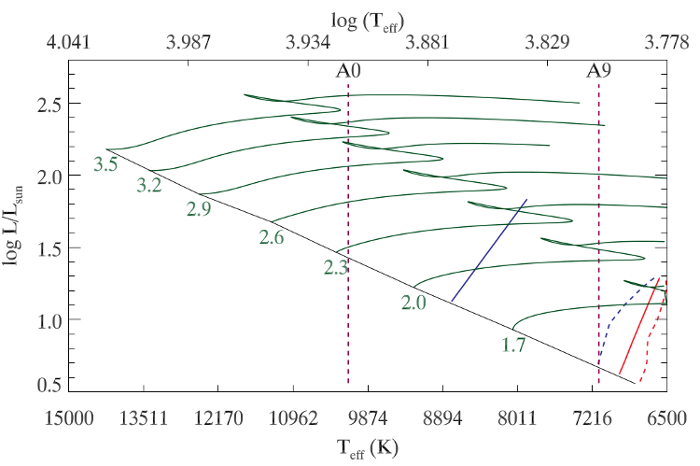
\includegraphics[width=\linewidth]{Chapter3/Astar_evol_tracks.png}
    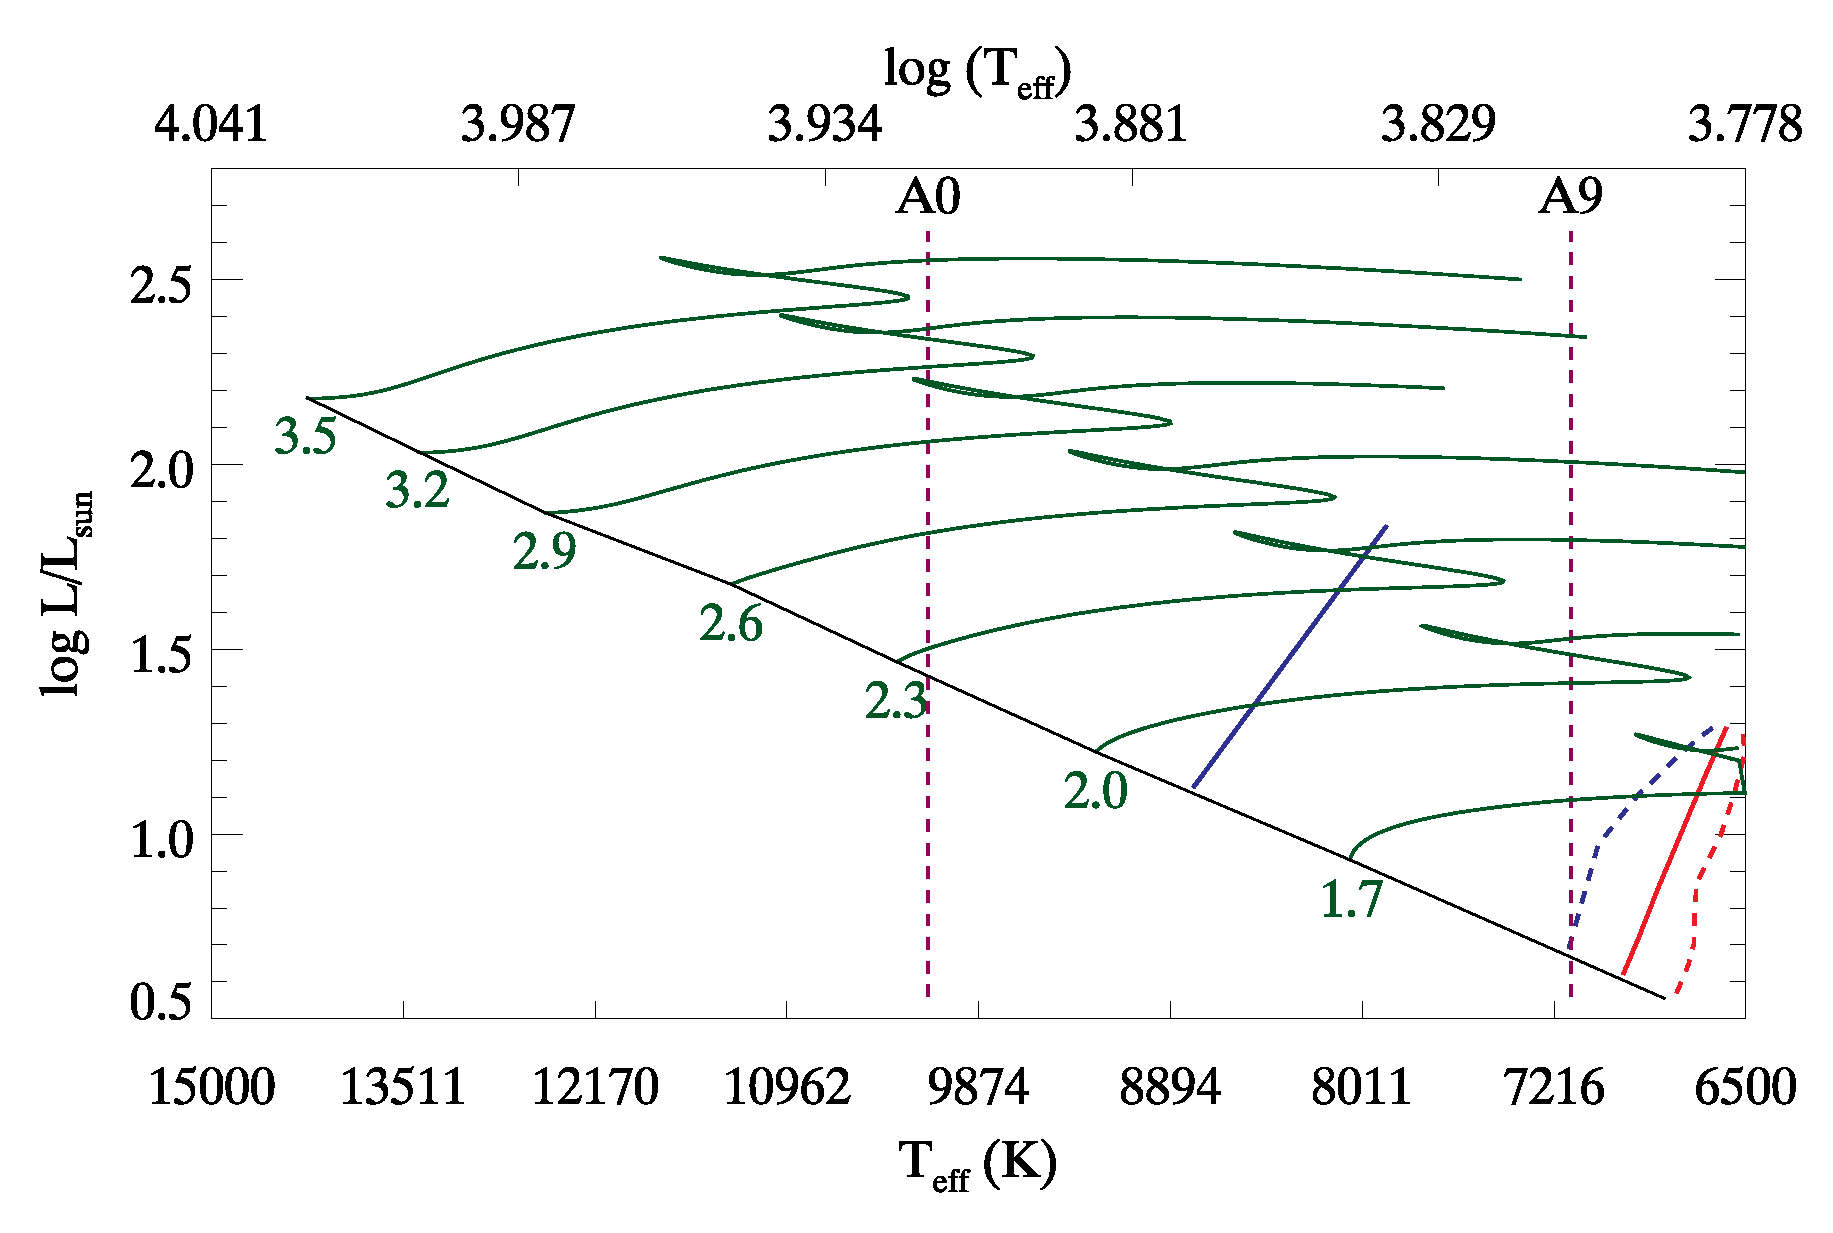
\includegraphics[width=\linewidth]{Chapter3/A_star_HR_delimited.eps}
    \caption[HR diagram with evolutionary tracks of A-type stars]{HR diagram between early-B and late-F spectral regions, reproduced from \citet{murphy_examination_2012}. Evolutionary tracks for 1.7\,\Msol~to 3.5\,\Msol~stars are plotted in green and corresponding masses given below the ZAMS (black). The A-type star boundaries are delineated with dashed purple lines at 10\,150\,K (A0) and 7\,150\,K (A9).}
    \label{fig:Astar_evol_tracks}
\end{figure}

% HR diagram covering the late-B to early-F region (spectral types A0
% and A9 are delimited). A star at A0 has a surface temperature of ∼10 150 K, and
% at A9 ∼7150 K. Evolutionary tracks are plotted in green, with their corresponding
% masses (in M ) written just below the zero-age main sequence (black). The principal
% direction of evolution for the B stars is to the right, such that they become A stars.
% For reference, the δ Sct instability strip’s red and blue edges are plotted as solid lines,
% and the γ Dor strip as dashed lines. Tracks were calculated using time-dependent
% convection (TDC) models, and contributed by A. Grigahcène (priv. comm.).

%As a class, the chemically peculiar A type (Ap) stars exhibit enhanced features of rare earth elements, such as Sr, Cr and Eu, in their spectra \citep{Morgan1933Evidence}. This enhancement is the result of a stable magnetic field on the order of a few to tens of kG \citep{Mathys2017Ap}, which typically allows for the formation of abundance `spots' on the surface, concentrated at the magnetic poles \citep{Ryabchikova2007Pulsation}. In most, but not all Ap stars, photometric and spectral variability over the rotation cycle can be observed \citep{Stepien2000Loss, Abt1995Relation}. Such characteristic spot-based modulation manifests as a low frequency modulation of the light curve which is readily identified, allowing for the rotation period to be measured \citep[e.g.][]{Drury2017Large}.
%As such, they are greatly outnumbered by the much more abundant non-oscillating Ap stars \citep{Renson2009Catalogue,Ghazaryan2018New}.

% Since their discovery by \citet{Kurtz1982Rapidly}, only 61 rapidly oscillating Ap (roAp) stars have been found. Understanding of their pulsation mechanism, occurrence rate, and origin of magnetic fields have all been hindered by the relatively small number of known roAp stars. A key difficulty in their detection lies in the rapid oscillations themselves, requiring dedicated observations from ground or space-based photometry at a short enough cadence to properly sample the oscillations. In this paper, we show that the \kepler\ long-cadence data can be used to detect roAp stars.

% The roAp stars are a rare subclass of the chemically peculiar A-type stars, which exhibit rapid brightness and radial velocity variations with periods between 5 and 25 min and amplitudes up to 0.018 mag in Johnson $B$ \citep{Kurtz2000Introduction, Kochukhov2009Asteroseismology, Smalley2015KIC}. They oscillate in high-overtone, low-degree pressure (p) modes \citep{Saio2005Nonadiabatic}. The excitation of high overtone p-modes, as opposed to the low overtones of other classical instability strip pulsators, is suspected to be a consequence of the strong magnetic field -- on the order of a few to tens of kG -- which suppresses the convective envelope at the magnetic poles and increases the efficiency of the opacity mechanism in the region of hydrogen ionisation \citep{Balmforth2001Excitation,Cunha2002Theoretical}. Based on this, a theoretical instability strip for the roAp stars has been published by \citet{Cunha2002Theoretical}. However, discrepancies between the observed and theoretical red and blue edges have been noted, with several roAp stars identified to be cooler than the theoretical red edge. 

% A further challenge to theoretical models of pulsations in magnetic stars is the existence of stars which oscillate above the so-called acoustic cutoff frequency \citep{Saio2013Pulsation,Holdsworth2018LCO}. In non-magnetic stars, oscillations above this frequency are not expected. However, in roAp stars the strong magnetic field guarantees that part of the wave energy is kept inside the star in every pulsation cycle, for arbitrarily large frequencies \citep{sousaandcunha2008}. For that reason, no theoretical limit exists to the frequency of the modes. Nevertheless, for a mode to be observed, it has to be excited. Models show that the opacity mechanism is capable of exciting modes of frequency close to, but below, the acoustic cutoff frequency. The excitation mechanism behind the oscillations with frequencies above the acoustic cutoff is thought to be turbulent pressure in the envelope regions where convection is no longer suppressed \citep{Cunha2013Testing}.

% The magnetic field axis of roAp stars is closely aligned with the pulsation axis, with both being inclined to the rotation axis. Observation of this phenomenon led to the development \citep{Kurtz1982Rapidly} and later refinement \citep{Dziembowski1985Frequency,Shibahashi1985Rapid,Shibahashi1985Rotational,Shibahashi1993Theory,Takata1994Selection,Takata1995Effects,Bigot2011Theoretical} of the oblique pulsator model. The roAp stars present a unique testbed for models of magneto-acoustic interactions in stars, and have been widely sought with both ground and space-based photometry.

\subsection*{Declaration}
The work presented in this publication was begun during my Honours year and completed in the course of this PhD. I extracted and processed the light curve using my own custom-defined aperture from superstamps that I stitched together. I conducted the Fourier analysis of the light curve searching for oscillation signatures and determined none were detectable above the signal-to-noise threshold. The multi-colour photometry was obtained by Aliz Derekas et. al. who eliminated the possibility of classification as a Cepheid for this star. The Nordic Optical Telescope (NOT) observations were conducted as part of the NOT `Fast-track' service time. Simon Murphy identified the chemically peculiar signatures of Europium, Strontium and Chromium as well as annotating the stellar spectrum. \'Ad\'am S\'odor conducted the model-based rotational modulation stability analysis that improved upon my initial polynomial-based O-C results. The analysis and writing of this paper was conducted by me in conjunction with my supervisors Dennis Stello and Tim Bedding.

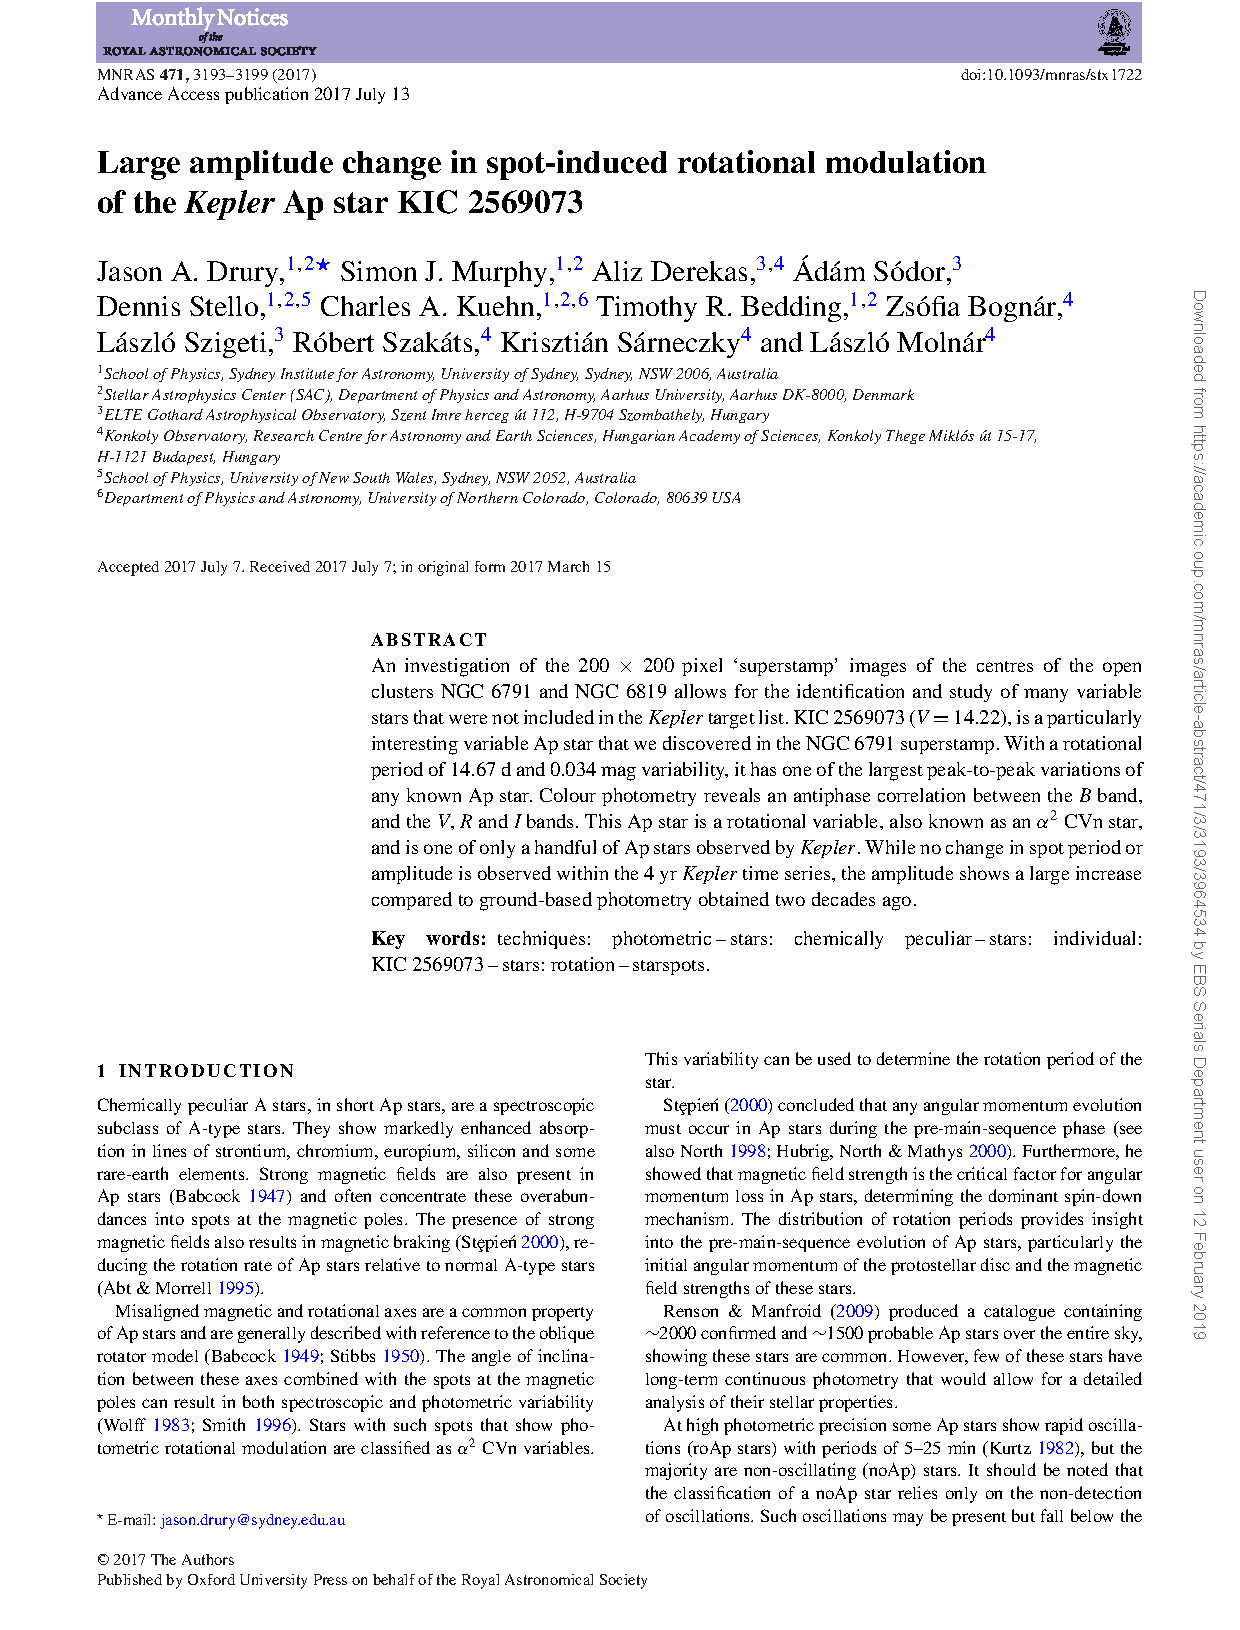
\includepdf[pages=-,pagecommand={},width=1.1\linewidth]{Papers_PDF/KIC2569073.pdf} % Work on superstamps and extraction.
\chapter[Gaia cluster membership]{Open cluster membership in the \Gaia~era}
\label{chap:membership}

\section*{abstract}
    In this chapter we present cluster membership lists for the four open clusters in the nominal \Kepler~field of view. We used a Gaussian Mixture Model (GMM) machine-learning algorithm to determine cluster membership using astrometric (position and proper motion) data from the \Gaia~space telescope. We produced a cross-matched database for the \Gaia~and \Kepler~stars in the cluster fields of view. Our cluster membership list contains 
\newpage
\section{Cluster membership}

NGC 6791
One of the most studied open clusters


Previous cluster membership of NGC\,6791 \& NGC\,6819.
Historical studies

\section{The {\em Gaia} Mission}
The \Gaia~space telescope is a European Space Agency (ESA) mission launched in 2013 into a Lissajous-type orbit around the Lagrange-2 (L2) point, 1.5\,Mkm from Earth, in the anti-Solar direction. It was primarily designed to produce a three-dimensional astrometric map of the Milky Way. The full science goals of the mission were; (1) to map the positions of approximately 1 billion stars in the Milky Way and Local Group (to a precision of 24\,$\mu$as at 15\,mag and 200\,$\mu$as at 20\,mag), (2) to measure the proper motion velocities of these stars, (3) to produce a 3D structural map of the Milky Way, (4) to provide spectral and photometric measurements for these stars, and (5) to provide radial velocities for the 150 million brightest stars.

% \newpage

Figure \ref{fig:Gaia_structure} shows a schematic diagram of the \Gaia~spacecraft modules; the payload module containing the single, integrated science instrument, the mechanical service module and the electrical service module. The service modules are combined in this schematic to form the equipped service module, with the propulsion tanks, solar panel arrays and phase array antenna situated below it.

\begin{figure}[h]
    \centering
    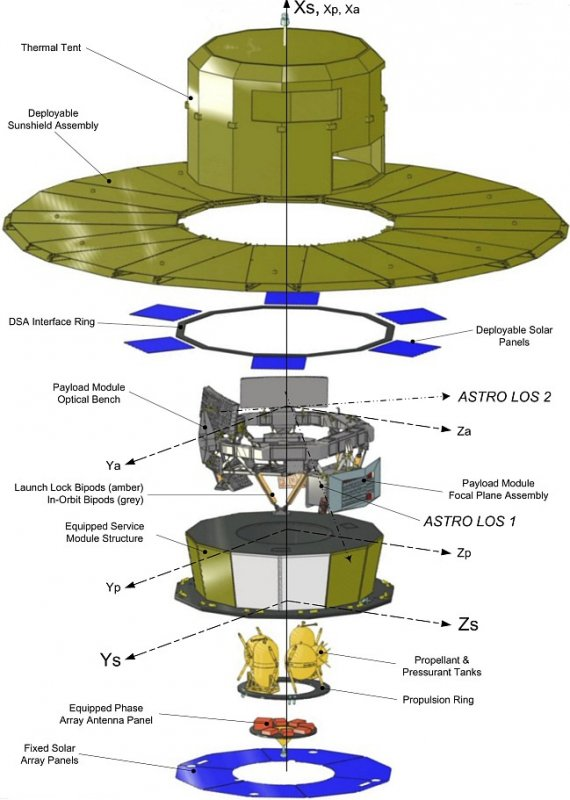
\includegraphics[width=0.6\linewidth]{Chapter4/gaia_schematic.jpg}
    \caption{Schematic diagram of the \Gaia~spacecraft. The electrical and mechanical service modules have been combined in this schematic into the `equipped service module structure', with the payload module displayed above.}
    \label{fig:Gaia_structure}
\end{figure}

The payload module contains the single, integrated instrument (Figure \ref{fig:gaia_instrument} (a)) responsible for delivering the astrometry, photometry and spectrometry data products. This instrument uses two identical telescopes with a shared focal plane, based on a three-mirror anastigmat design. A detailed schematic view of the optical path to the detector is shown in Figure \ref{fig:gaia_instrument} (b). The focal plane of the detector (Figure \ref{fig:gaia_focalplane}) has dimensions of 0.5\,m $\times$ 1.0\,m and consists of 106 CCDs that provide dedicated channels for each data product.

\begin{figure}[h]
    \centering
    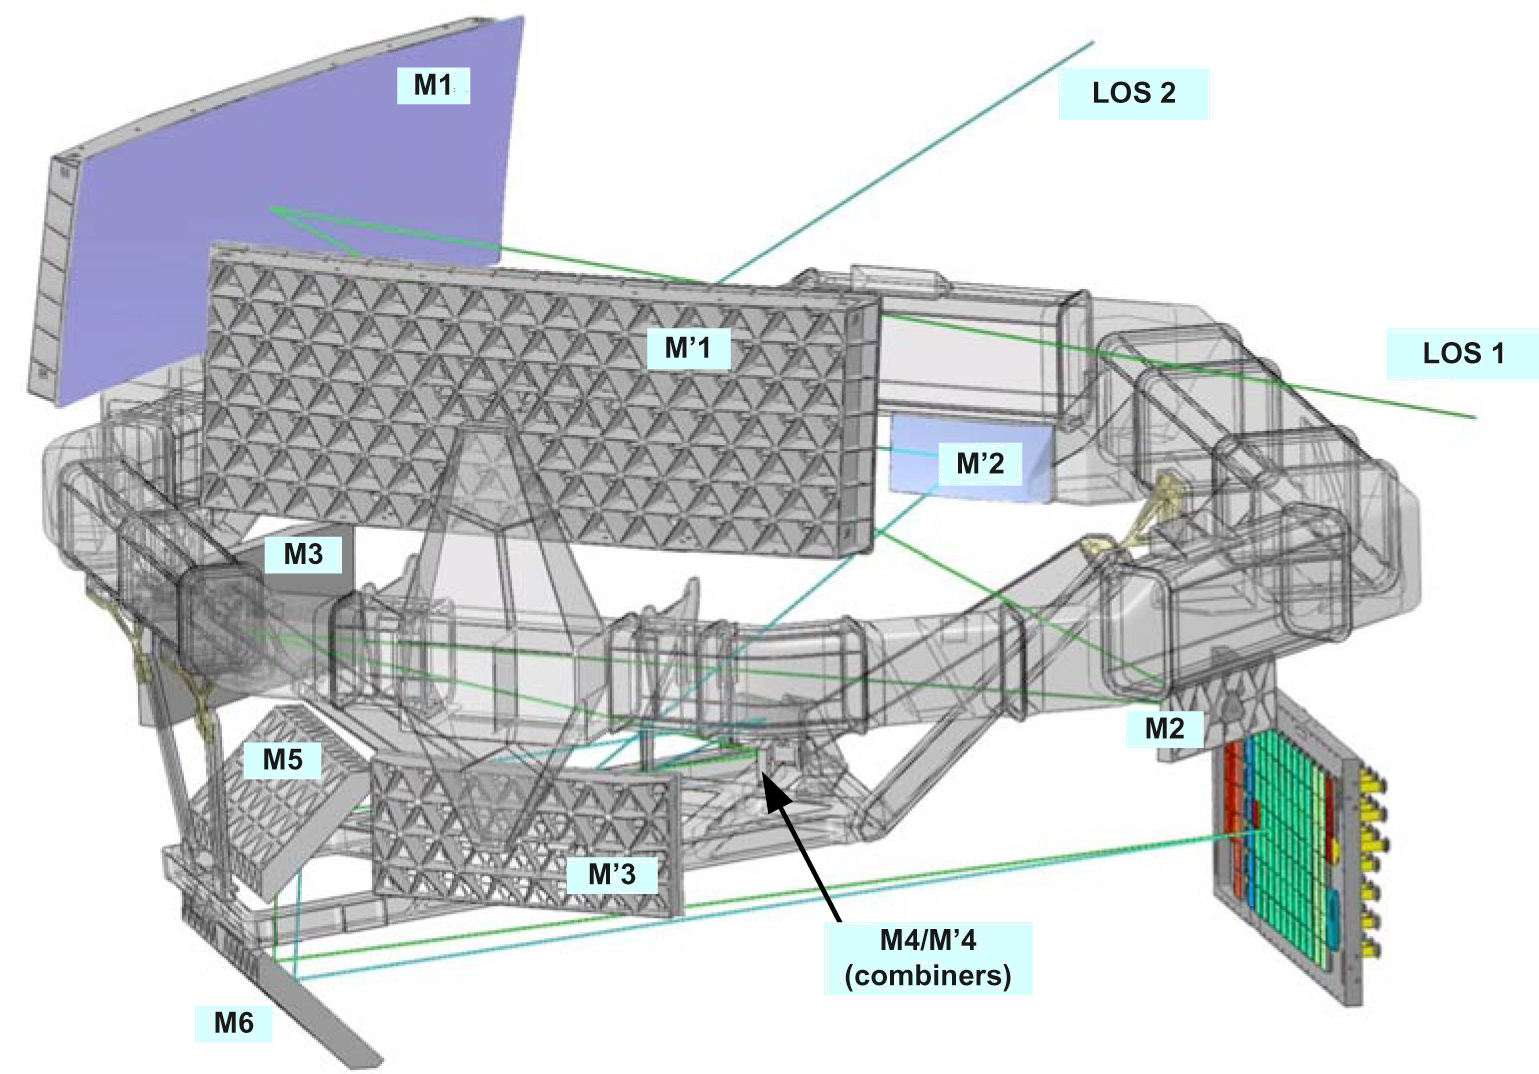
\includegraphics[width=0.8\linewidth]{Chapter4/gaia_optics.png}\\
    \vspace{25pt}
    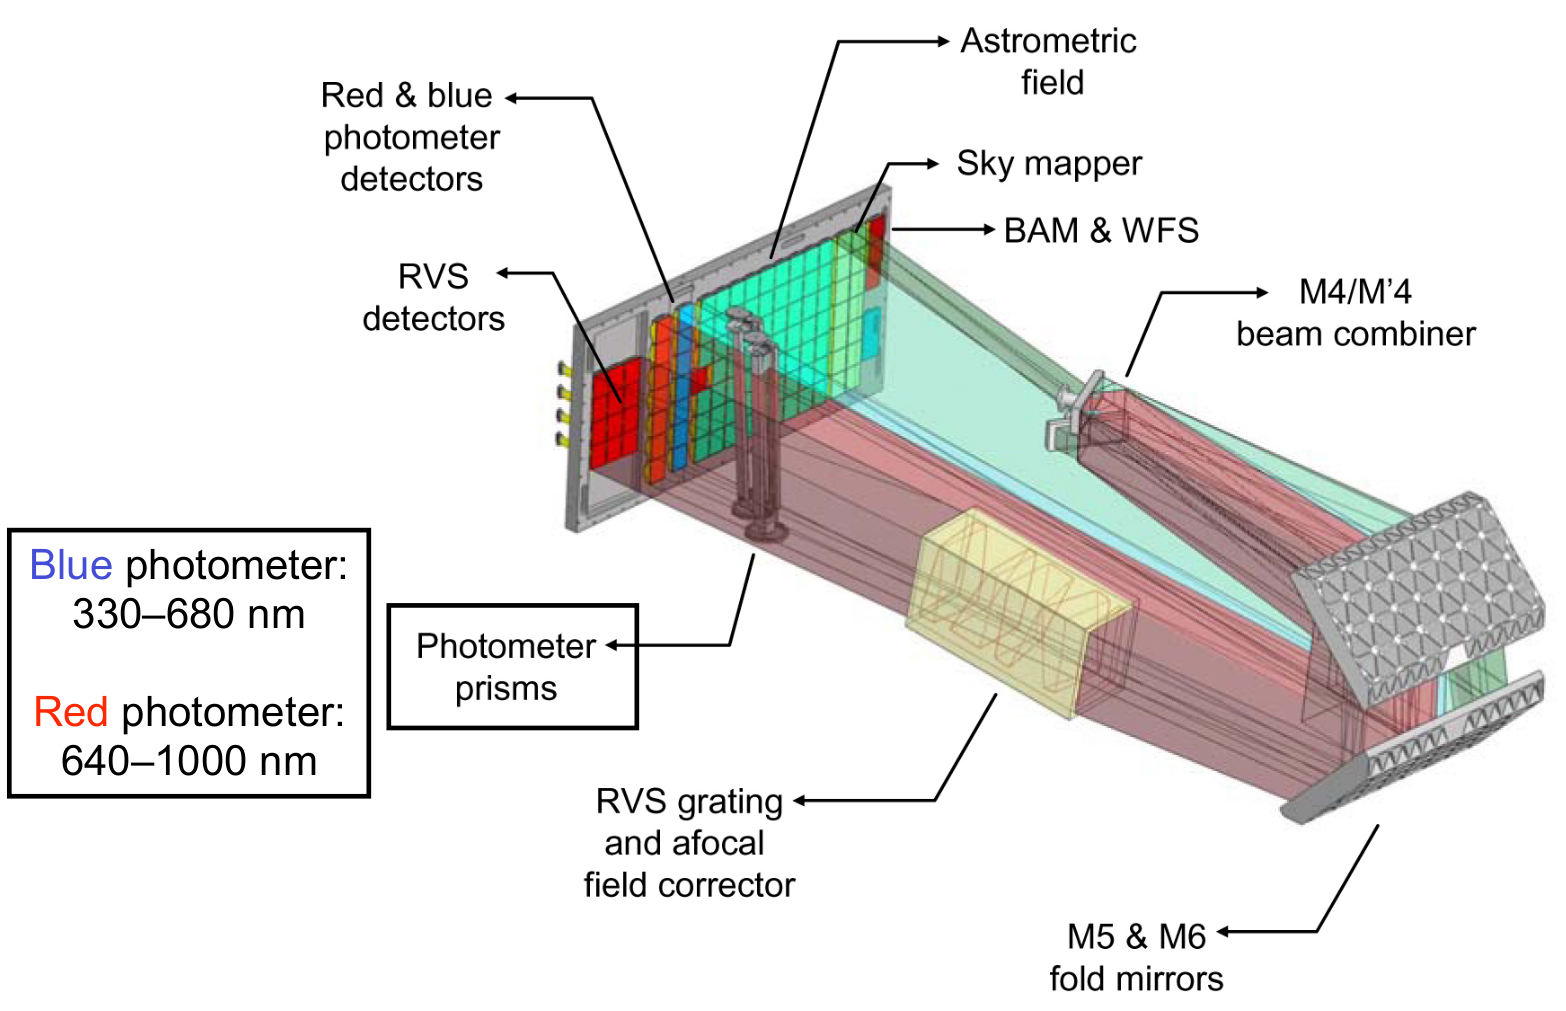
\includegraphics[width=0.8\linewidth]{Chapter4/gaia_foc.png}
    \caption{Schematic diagrams of (a) The \Gaia~optical instrument bench, and (b) The optical ray path from the M4/M'4 beam combiner to the focal plane containing the CCD detectors.}
    \label{fig:gaia_instrument}
\end{figure}

\begin{figure}[h]
    \centering
    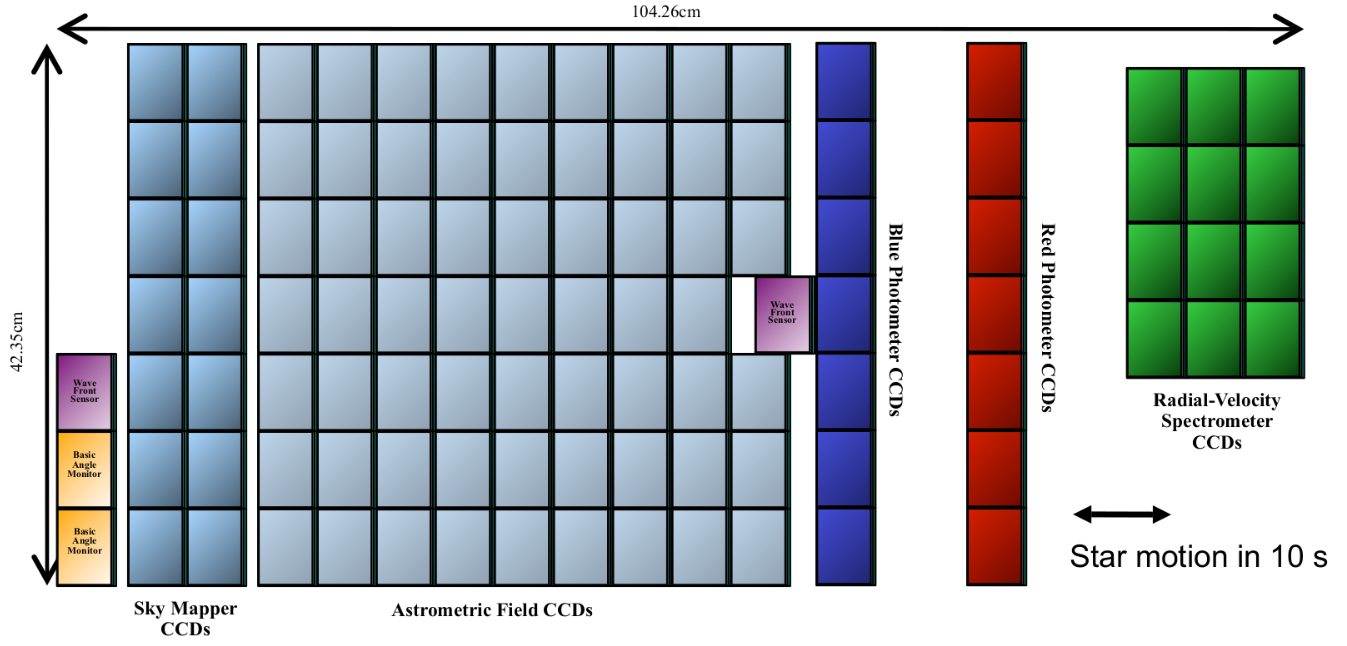
\includegraphics[width=0.9\linewidth]{Chapter4/gaia_detect_edit.png}
    \caption{Schematic diagram of the \Gaia~focal plane consisting of 106 CCDs, with the positions and dedicated instrument allocation of individual CCD modules annotated.}
    \label{fig:gaia_focalplane}
\end{figure}

\subsection{Astrometry}
The latest data release for the \Gaia~mission, Gaia DR2 (hereafter DR2), occurred in April 2018 \citep{gaia_collaboration_gaia_2018}. It contained five-parameter astrometric solutions ($\alpha$, $\delta$, $\mu_{\alpha}$, $\mu_{\delta}$, $\pi$) for 1.7\,billion stars, combined with photometric and spectrometric (G, G$_{BP}$, G$_{RP}$) magnitudes for 1.3\,billion stars. \citet{bailer-jones_estimating_2018} computed geometric distance estimates for all stars with a parallax in the DR2 release. We use both of these data products for the following analysis.

\section{Clustering methods}
We investigated a number of clustering algorithms to identify probable cluster members including Mean-Shift Clustering, Density-based Spatial Clustering of Applications with Noise (DBSCAN), and Expectation–Maximization (EM) clustering using Gaussian Mixture Models (GMM). We provide a description of how these algorithms function below, and discuss the benefits and limitations of each.

\subsection{Mean-Shift Clustering}

The mean-shift clustering algorithm locates local over-densities in N-dimensional data using a centroid-based, sliding window. The algorithm begins with a randomly-selected initialisation point at the centre of a radially-profiled kernel (e.g circular window in 2-D) in the parameter space. This kernel is iteratively shifted to higher density regions by calculating the mean of all enclosed points. The iterative shifting is concluded when the total number of points within the window no longer increases and convergence is achieved. 

This process is repeated with additional kernels until every data point in the parameter space is contained within a window, and thus assigned to a particular cluster. If multiple windows overlap, the window with the greatest density is preserved as the parent cluster, and the remaining windows eliminated.

The primary benefit of the mean-shift clustering algorithm is its ability to locate clusters without prior knowledge of the number of clusters present. This is offset by the need to tune the kernel radius hyper-parameter, a task that may be non-trivial. This process returns a binary classification of cluster membership and does not account for data points that may not be related to any particular cluster (ie noise).

\vspace{10pt}

\noindent{\bf Pros}: 
\begin{itemize}
    \item Automatically determines the number of clusters so no prior knowledge of clusters required.
\end{itemize} 

\noindent{\bf Cons}: 
\begin{itemize}
    \item Selection/tuning of the kernel radius hyper-parameter can be non-trivial.
    \item Binary classification to cluster only (member/non-member).
    \item Cannot account for noise in data set.
    \item Cannot account for clusters of varied density.

\end{itemize}

\subsection{Density-based Spatial Clustering of Applications with Noise (DB-SCAN)}

DB-SCAN is a classification algorithm designed to locate clusters of over-density within a given parameter space whilst accounting for the presence of non-members. 

The algorithm selects an arbitrary initialization point and calculates a distance metric for the given parameter space to all other data points. If there are a sufficient number of points, \texttt{min\_points}, within a given maximum separation, $\epsilon$, it classifies the point as belonging to a cluster, otherwise it is classified as noise. All data points within the $\epsilon$ distance vector of a cluster member are associated with the same cluster, and the classification repeated iteratively for each point, until all points within the $\epsilon$ neighborhood of the cluster have been added. This process is repeated for all unclassified data points, until all points have been assigned to a cluster or classified as noise.

DB-SCAN's main advantage over mean-shift clustering is the ability to account for noisy data where no cluster assignment is valid. It is also capable of locating clusters of arbitrary shapes and sizes. As with mean-shift clustering, DB-SCAN has difficulty accounting for varied cluster density, as the hyper-parameters will change from cluster to cluster. Tuning the hyper-parameters to account for normalised distances between parameter spaces can also be difficult, particularly with high-dimensional data.

\vspace{10pt}

\noindent{\bf Pros}: 
\begin{itemize}
    \item Automatically determines the number of clusters so no prior knowledge of clusters required.
    \item Can account for arbitrary cluster shapes and sizes.
    \item Can account for noisy data.
\end{itemize} 

\noindent{\bf Cons}: 
\begin{itemize}
    \item Selection/tuning of the distance, $\epsilon$, and minimum cluster members, \texttt{min\_points}, hyper-parameters can be non-trivial.
    \item Normalising dimensions, and thus calculating the $\epsilon$ hyper-parameter for high-dimensional data can be difficult.
    \item Binary classification to cluster only (member/non-member).
    \item Cannot account for clusters of varied density.
\end{itemize}

\subsection{Hierarchical DBSCAN (HDBSCAN)}

HDBSCAN is a variation of the traditional DBSCAN algorithm. It uses a hierarchical clustering algorithm to compensate for differences in cluster densities, allowing the identification of multiple clusters with different densities. 

hierarchical clustering algorithm, and then using a technique to extract a flat clustering based in the stability of clusters.

\subsection{Expectation-Maximization (EM) using Gaussian Mixture Modelling (GMM)}

Gaussian Mixture Models (GMMs) give us more flexibility than K-Means. With GMMs we assume that the data points are Gaussian distributed; this is a less restrictive assumption than saying they are circular by using the mean. That way, we have two parameters to describe the shape of the clusters: the mean and the standard deviation! Taking an example in two dimensions, this means that the clusters can take any kind of elliptical shape (since we have standard deviation in both the x and y directions). Thus, each Gaussian distribution is assigned to a single cluster.

In order to find the parameters of the Gaussian for each cluster (e.g the mean and standard deviation) we will use an optimization algorithm called Expectation–Maximization (EM).

We begin by selecting the number of clusters (like K-Means does) and randomly initializing the Gaussian distribution parameters for each cluster.
Given these Gaussian distributions for each cluster, compute the probability that each data point belongs to a particular cluster. The closer a point is to the Gaussian’s center, the more likely it belongs to that cluster. This should make intuitive sense since with a Gaussian distribution we are assuming that most of the data lies closer to the center of the cluster.
Based on these probabilities, we compute a new set of parameters for the Gaussian distributions such that we maximize the probabilities of data points within the clusters. We compute these new parameters using a weighted sum of the data point positions, where the weights are the probabilities of the data point belonging in that particular cluster.
Steps 2 and 3 are repeated iteratively until convergence, where the distributions don’t change much from iteration to iteration.There are really 2 key advantages to using GMMs. Firstly GMMs are a lot more flexible in terms of cluster covariance than K-Means; due to the standard deviation parameter, the clusters can take on any ellipse shape, rather than being restricted to circles.Secondly, since GMMs use probabilities, they can have multiple clusters per data point. So if a data point is in the middle of two overlapping clusters, we can simply define its class by saying it belongs X-percent to class 1 and Y-percent to class 2. I.e GMMs support mixed membership.


\subsection{More realistic modelling}

\section{Methodology}

We used Gaussian Mixture Modelling (GMM) to calculate the posterior probability of membership for all stars within pre-determined radii of the four open clusters in the nominal \Kepler~field of view. We selected these radii to be approximately 2.5 times the literature reported radius for each cluster to ensure no potential cluster members were missed. Table \ref{tab:cluster_selection} presents the positions and radial distance cuts we used for each cluster. 

\vspace{3pt}

\begin{table}[h]
    \centering
    \setlength\tabcolsep{10pt}
    \begin{tabular}{ccccc}
        \hline
        Cluster     & RA        & Dec       & Radius    & Radial distance cut \\
                    &           &           & (arc mins)& (arc mins) \\
        \hline
        \hline
        NGC 6791    & 290.2208  & 37.771    & 23.0\footnote[2]{$r_t$ - Tidal radius \citep{platais_new_2011}} & 60.0\\
        NGC 6819    & 295.325   & 40.1867   & 15.0\footnote[2]{\citet{yang_wiyn_2013}} & 48.0\\
        NGC 6811    & 294.3208  & 46.3883   & 7.0               & 17.5\\
        NGC 6866    & 300.9792  & 44.1583   & 13.0              & 32.5\\
        \hline
    \end{tabular}
    \caption{Properties of open clusters in the \Kepler~FoV and the radial distance cut used for each cluster for cross-matching the \Gaia~and \Kepler~catalogs.}
    \label{tab:cluster_selection}
\end{table}

Data selected to try to ensure as close to complete membership as possible. Download \Gaia~DR2 data for all stars within the cutoff radius of the cluster centres. Due to distance of NGC 6819 \& 6791 we do not make a magnitude cut of this point despite the significant decrease in astrometric quality for stars fainter than G = 20 mag. Only a small fraction have RVs, with almost none of the cluster members from NGC 6791 having such values, so not used. Similarly, parallax values for these clusters are very small (distances are ~2 \& ~4 kpc respectively) meaning there is a very large uncertainty on their measurements. Due to this we did not use the parallax in the clustering analysis (See \cref{sect:cuts})

As reported by Lindegren et al. (2018) and confirmed
by several other works (Riess et al. 2018; Stassun &
Torres 2018; Zinn et al. 2018), there is a zero-point offset
in the Gaia DR2 parallaxes that needs to be considered.
While this zero-point itself is a function of position and
magnitude, for the remainder of this paper we adopt the
global mean value of 29μas (in the sense that the Gaia
parallaxes are too small) reported by Lindegren et al.
(2018).

In order to derive reliable values for the cluster and
field parameters, we have used the subset of our initial
pool of stars that pass the quality cuts impossed by Zinn
et al. (2018) (which ensure a good astrometric solution)
and that are within 20 0 of the cluster center.(For similar samples in larger areas the field population is so dominant over the cluster that the latter becomes negligible and the method does not converge).

We used the position ($\alpha$ and $\delta$) and proper motion ($\mu_{\alpha}$ and $\mu_{\delta}\dot~cos\delta$) parameter space for all \Gaia~sources within the cutoff radius in our gaussian mixture model analysis. 
run sklearn gmm on (pmra,pmdec,ra,dec) with n components (6791 = 6, 6819 = 12). n$_{}$comp chosen based on initial runs where the minimum number of components needed to converge to cluster members is accepted. Iteratively repeat using Monte Carlo (gaussian function over ($pmra_err,pmdec_err,ra_err,dec_err$)) to sample the parameter space. Accept cluster if 50$\%$ of members from initial run included in one component of the current GMM convergence, otherwise reject.

Cluster:	6819 | 6791	
Position:	[295.325, 40.1867] | [290.2208, 37.771]
radius cut:	0.8	| 1.0
gmm tol:	1e-5       
gmm maxiter:	20000      
gmm cov:	full       
gmm weight:	dirichlet distribution

Include the images showing the probability distribution of highly-likely, likely, non-likely members and some which are ambiguous.

Describe choices made about membership and show results.

6791


6819

\section{Results}

\label{sect:cuts}

\begin{figure}
\centering
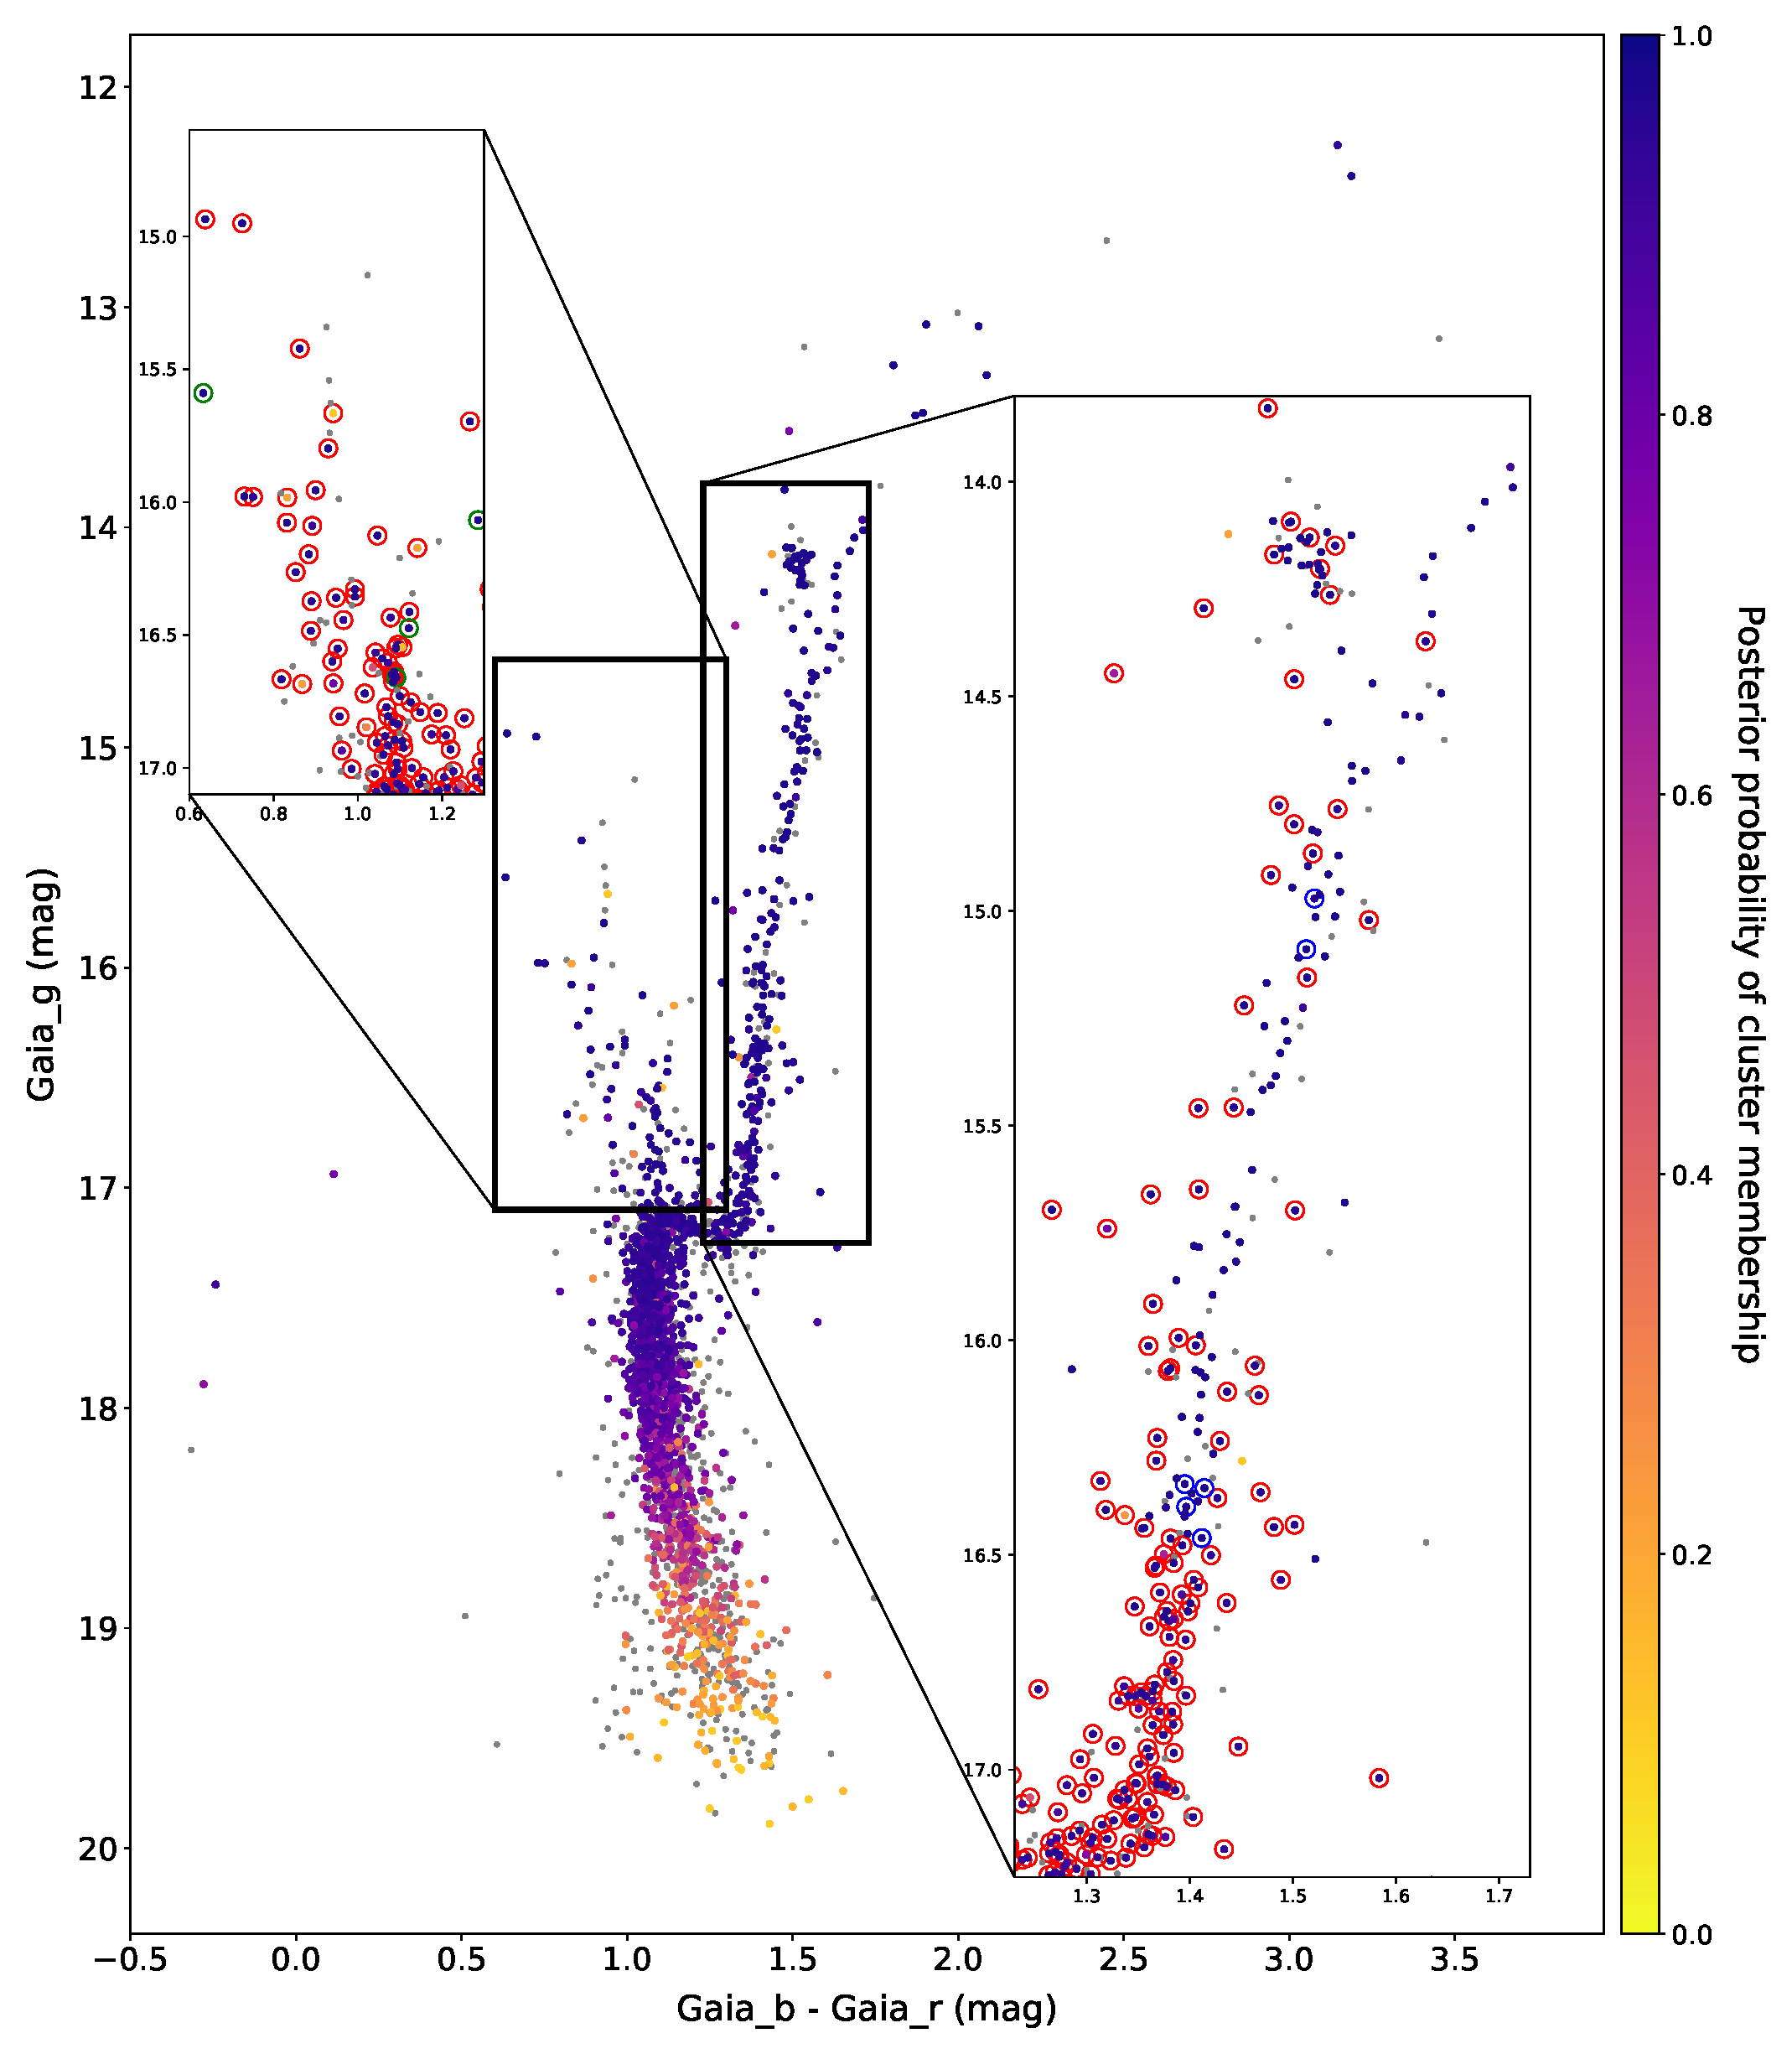
\includegraphics[width=\linewidth]{Chapter4/cmd_6791.eps}
\caption[NGC\,6791 CMD]{Colour magnitude diagram of NGC\,6791 based on \Gaia~$g$ and $b-r$ passband photometry, showing likely cluster members (gray) with those that fall inside the \Kepler~super stamps shaded by their posterior probability of membership. The red giant branch (right insert) and blue straggler stars (left insert) are highlighted. For these regions we have further highlighted the non-targeted super stamp stars (red circles, both), red giants observed for less than nine quarters (blue circles, right), and observed blue stragglers (green circles, left)}
\end{figure}

\begin{figure}
\centering
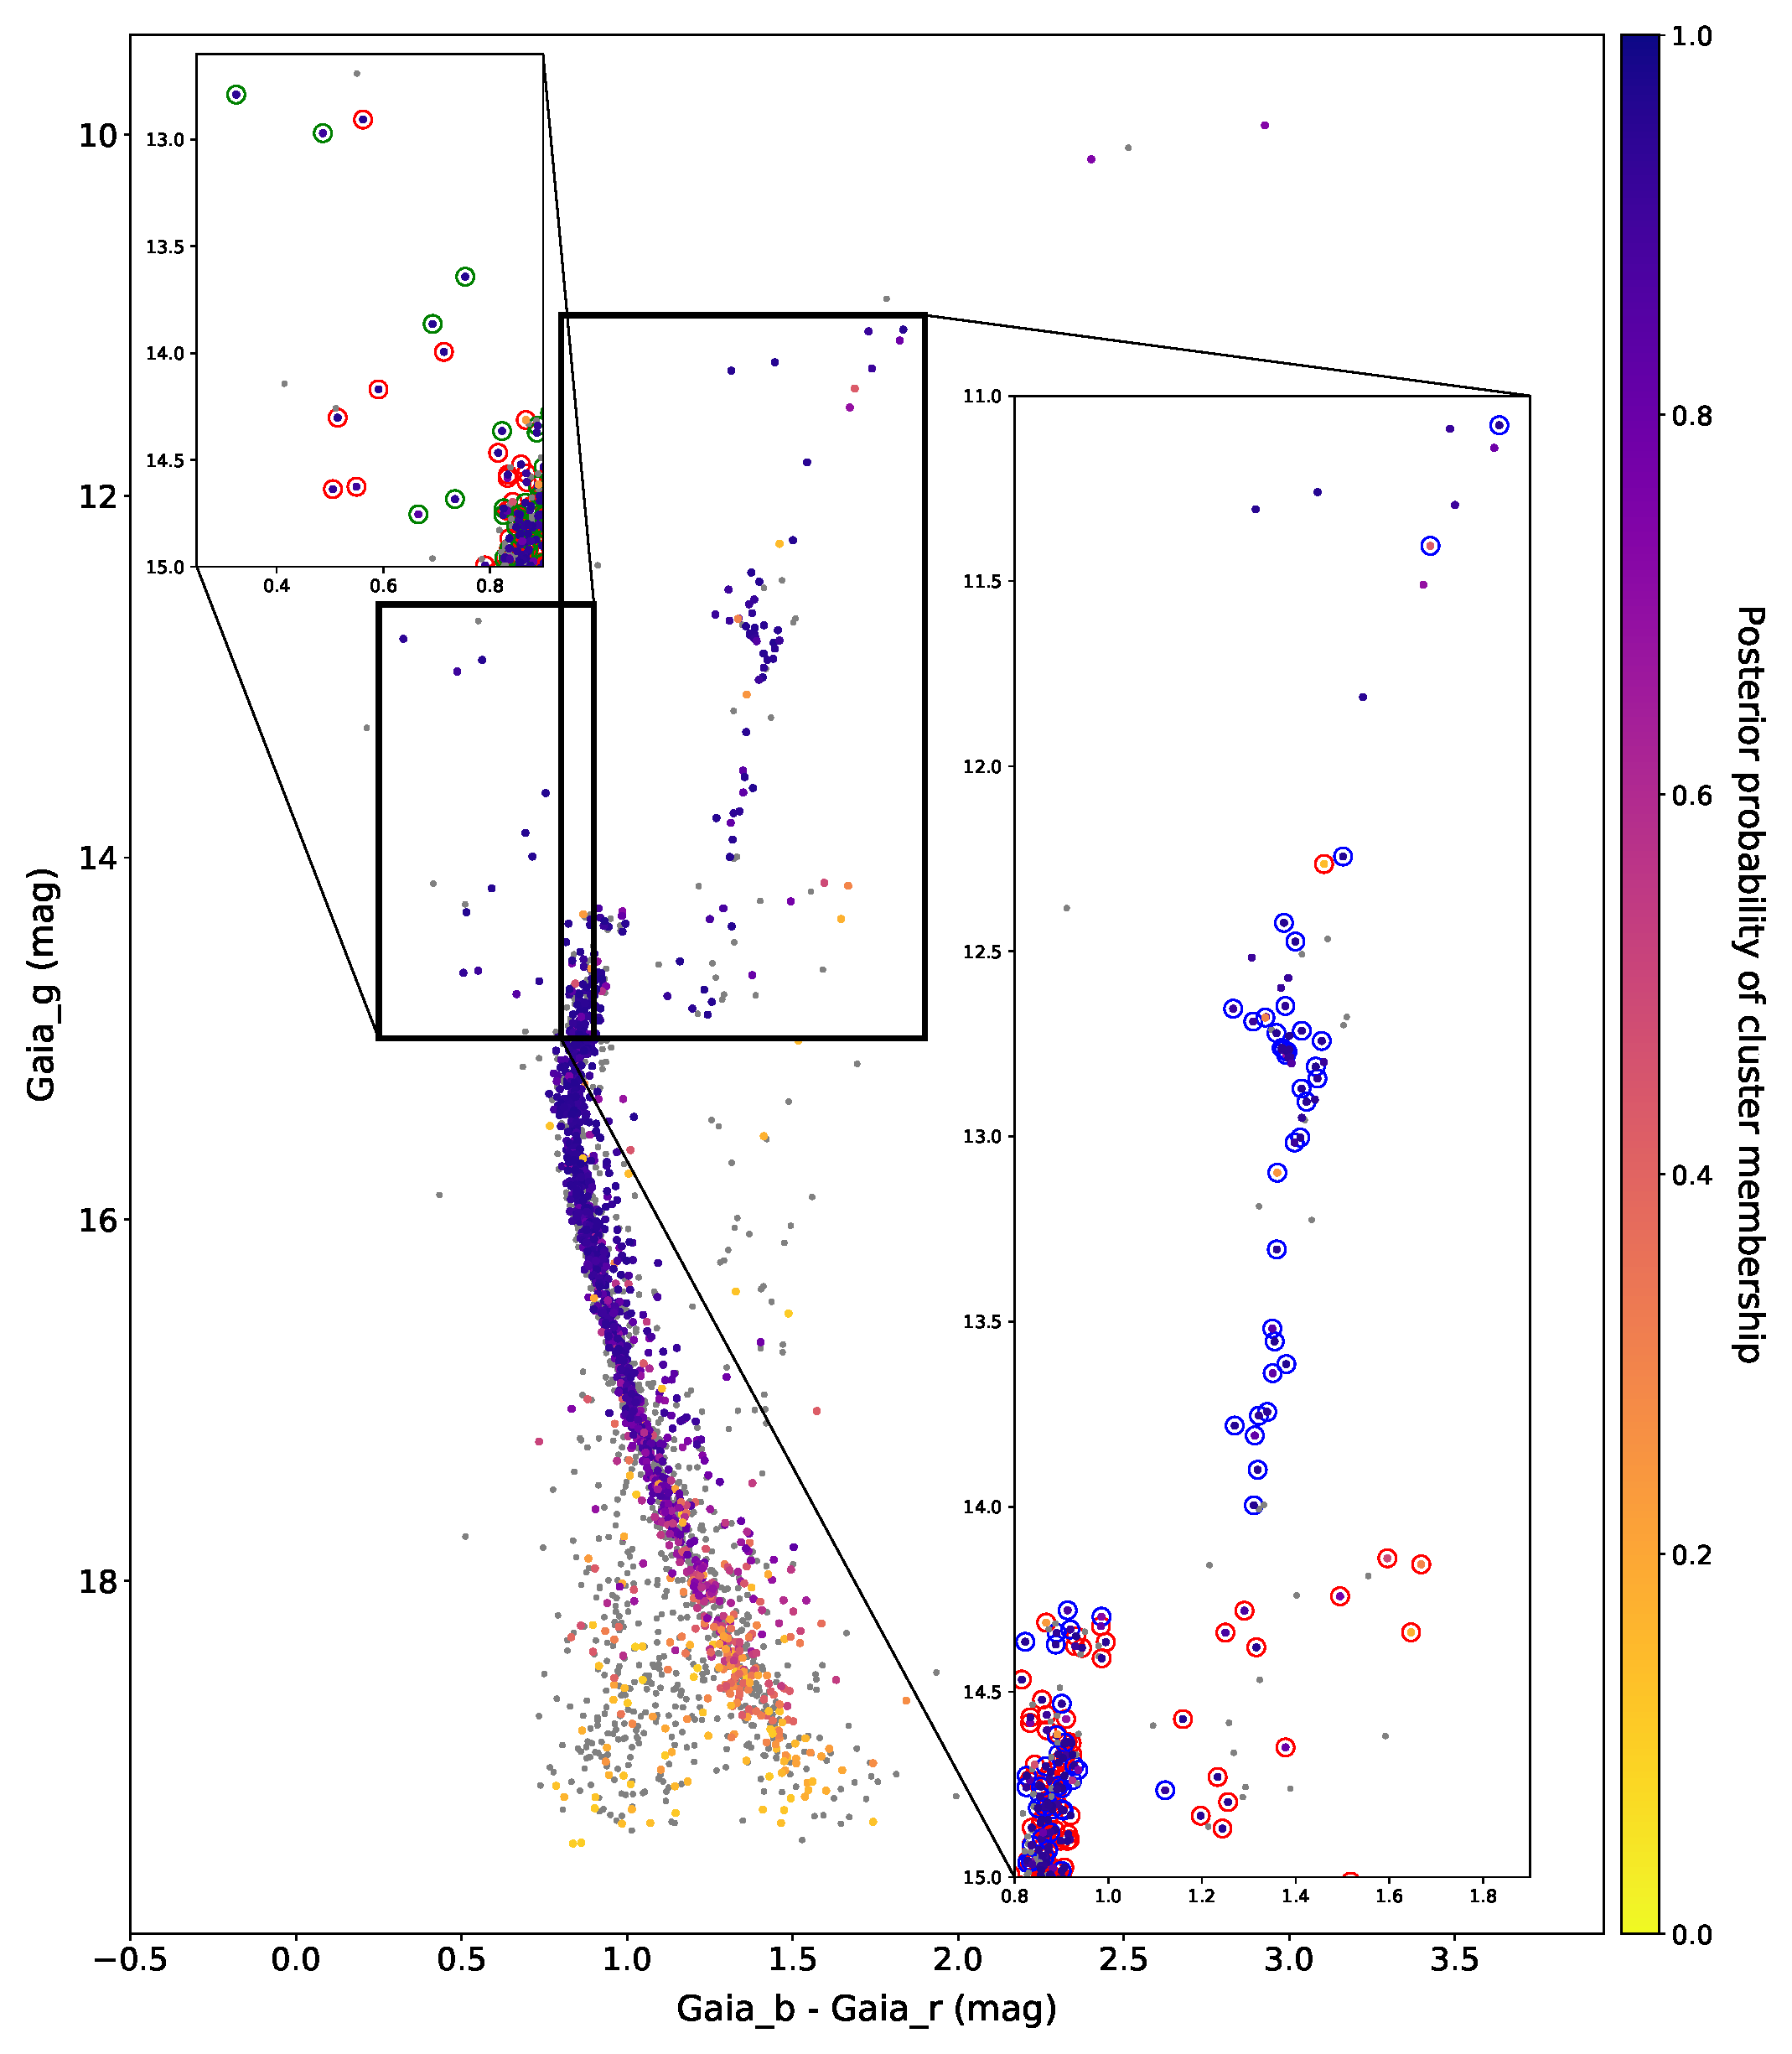
\includegraphics[width=\linewidth]{Chapter4/cmd_6819.eps}
\caption[NGC\,6819 CMD]{Colour magnitude diagram of NGC\,6819 based on \Gaia~$g$ and $b-r$ passband photometry, showing likely cluster members (gray) with those that fall inside the \Kepler~super stamps shaded by their posterior probability of membership. The red giant branch (right insert) and blue straggler stars (left insert) are highlighted. For these regions we have further highlighted the non-targeted super stamp stars (red circles, both), red giants observed for less than fifteen quarters (blue circles, right), and observed blue stragglers (green circles, left)}
\end{figure}

\subsection{Kepler-Gaia DR2 Cross-matching}

% To combine this astrometric analysis with the photometric (and thus asteroseismic) {\em Kepler} information we need to match the {\em Kepler} and {\em Gaia} identifiers.

\citet{berger_revised_2018} produced a \Gaia~cross-matched database for all \Kepler~targeted stars to allow for astrometric analysis of these stars, but excluded non-targeted cluster stars. We have now extracted light curves for many of these non-targeted stars within the centres of the open clusters in the nominal \Kepler~FoV from the \Kepler~superstamps (%\citet{Colman19}, 
Ch. \ref{chap:lightcurves}). These stars are now of particular interest in terms of cluster membership for conducting ensemble asteroseismic analyses, and require a cross-match between \Kepler~and \Gaia~identifiers.

% Before cross-matching the \Gaia~and \Kepler~catalogs, we converted the Gaia stellar positions ($\alpha$, $\delta$) from the J2015.5 reference frame to the J2000.0 reference frame used by the \Kepler~Input Catalog (KIC) \citep{brown_kepler_2011}. 
Before cross-matching the \Gaia~and \Kepler~catalogs, we corrected the Gaia stellar positions ($\alpha$, $\delta$) for proper motion to the J2000.0 epoch. We then restricted the cross-match to stars within a radius of each cluster centre matching the cluster radius selected for the cluster membership analysis (see Table \ref{tab:cluster_selection}). 

To begin the cross-match, we removed all KIC stars without a \Kepler~magnitude (Kp). For every \Gaia~star, we selected all matches within an initial 3 arcsecond radius. We further filtered the matches by imposing a magnitude cut based on the \Gaia~g-band photometry and \Kepler~magnitude to ensure ${|g-Kp| \leq 2}$, and selected the closest star as the best match. For any duplicate \Kepler~matches we selected the \Gaia~match with the smallest angular separation as the best match. We then removed this \Kepler~match from the possible matches, and iteratively repeated the cross-match until all stars were matched or no match was found. 

Finally, we removed all matches with angular separations greater than 1.5 arcseconds. We selected 1.5 arcseconds based on a 5\,$\sigma$ interval from a truncated Gaussian fit to the angular separation distribution. We assume any matches beyond this angular separation are likely to be spurious background or foreground contaminants as suggested by \citet{berger_revised_2018}. We present the number of stars included at each stage of the cross-match, for each cluster field of view, in Table \ref{tab:cluster_crossmatch}.

%Could not use APASS gri photometry to fill in Kepler data and generate predicted G mag as Berger due to cluster members typically being much fainter than the limiting cutoff mag for APASS.
\begin{table}[h]
    \centering
    \setlength\tabcolsep{10pt}
    \begin{tabular}{ccccc}
        \hline
        % Cluster     & RA        & Dec       & Radius    & Radial distance cut \\
        %             &           &           & (arc mins)& (arc mins) \\
        % \hline
        % \hline
        % NGC 6791    & 290.2208  & 37.771    & 23.0\footnote[2]{$r_t$ - Tidal radius \citep{platais_new_2011}} & 60.0\\
        % NGC 6819    & 295.325   & 40.1867   & 15.0\footnote[2]{\citet{yang_wiyn_2013}} & 48.0\\
        NGC 6811    & 294.3208  & 46.3883   & 7.0               & 17.5\\
        NGC 6866    & 300.9792  & 44.1583   & 13.0              & 32.5\\
        \hline
    \end{tabular}
    \caption{Number of stars present in the cross-matched database at each stage.}
    \label{tab:cluster_crossmatch}
\end{table}


NGC 6791  [125\,018 KIC stars and 153\,626 \Gaia~stars] to begin the cross-match.




% For stars with multiple matches that satisfied these criteria, we decided to keep those with the smallest angular separations. Of the 197,104 stars present in the KSPC, we identified Gaia DR2 source matches for 195,710. Stars with poorly determined parallaxes (σ π /π > 0.2), low effective temperatures based on our adopted values (T eff < 3000 K, see Section 2.2), extremely low log g (< 0.1 dex), and/or non-“AAA”-quality Two Micron All Sky Survey (2MASS) photometry were rejected from our sample.

% Additionally, we made astrometric cuts similar to those described in Appendix C of Lindegren et al. (2018) and Section 4.1 of Arenou et al. (2018). In particular, we used Equation (1) (unit weight error compared to a function of the G magnitude of the source that helps filter contamination from binaries and calibration problems) and Equation (3) (greater than eight groups of observations separated by at least 4 days) of Arenou et al. (2018) to remove stars with bad astrometric solutions. We did not use the astrometric excess noise values provided by Gaia DR2 to filter stars because they were less discriminating for stars with G < 15 due to the “degree of freedom bug” (see Appendix A and C of Lindegren et al. 2018). We did not use Equation (2) of Arenou et al. (2018), a cut ensuring that Gaia has clean photometry of the included sources, because we utilized separate 2MASS photometry in our analysis. As discussed in Lindegren et al. (2018), our imposed cuts removed many stars that appear in unphysical areas of radius-T eff parameter space, such as the “subdwarfs” between the stellar main sequence and the white dwarf branch. Excluding these stars reduced our final sample to 177,911 Kepler stars.

% Methodology:
% Position, pm and colour-photometry from Gaia - g, b, r => Conversion to Kepler (Kp) magnitudes

% Match on Kp (calculated) and measured -> remove any greater than 2mags
% Closest match

% Results:

Database of Kepler and Gaia ID's including the information from both databases. (Include table of ~20 examples [<= 1 page] with extended match online) % Work on cluster membership
\chapter{Photometry of NGC\,6791 \& NGC\,6819 Red Giant Cluster Members}
\label{chap:red_giants}

% \section*{abstract}
%     In this chapter we present global asteroseismic parameters for all red giant (RG) cluster members of NGC\,6791 and NGC\,6819. We selected these RGs based on our membership determinations from the previous chapter. We corrected the instrumental perturbations present in the raw light curves for all red giant cluster member candidates and selected the light curve corrections resulting in the highest red giant excess signal-to-noise. We present a complete database of the extracted global asteroseismic parameters of $\nu_\mathrm{max}$, $\Delta\nu$, $\epsilon$, and the stellar granulation parameters, and compare the cluster ensembles to the full \Kepler{} targeted ensemble.
\newpage

\section{Introduction to Solar-like oscillators}

\cite{leighton_velocity_1962} first observed the five minute oscillations in the Sun. These are now known to be stochastically driven and intrinsically damped by turbulent motion in the convective envelope. Solar-like oscillators refers to all variable stars with oscillation modes excited through this process of stochastic turbulence in the convective envelope. Therefore, these oscillations should be present in any star with a significant convective envelope, including low-mass (M $\leq 1.6$\,\Msol{}) main sequence stars, subgiant stars and red giant stars \citep{aerts_current_2008}. 

Solar-like oscillation modes typically exhibit p-mode behaviour in the convective envelope, where they are predominantly acoustic in character with a pressure-driven restoring force. Theory also predicts g-mode behaviour in the core, where buoyancy is the restoring force. Figure \ref{fig:modes} shows ray paths for p-modes (left) and g-modes (right) within a solar-like star. The p-modes penetrate deeper into the stellar interior when they are of lower angular degree, whilst g-modes are typically restricted to the radiative core, being evanescent in stellar convective zones.

As discussed in \cref{chap:intro:astero}, we can detect these oscillations by taking precise measurements of photometric changes. There have been a number of space-based missions over the past two decades including \textsc{Most} \citep{rucinski_most_2003}, \textsc{CoRoT} \citep{michel_corot_1998}, \Kepler{} and \textit{K2} \citep{borucki_kepler_2009}, and now \textsc{Tess} \citep{ricker_transiting_2014}, that have provided high-precision photometric data for thousands of solar-like stars. This data has led to a revolution in our understanding of their stellar structure and processes. Many large surveys of solar-like oscillators have been conducted \cite[eg.][]{stello_detection_2010,hekker_characterization_2011,mosser_characterization_2012,mosser_mixed_2014,yu_asteroseismology_2018-1} with \cite{hon_search_2019} having conducted the largest and most comprehensive search for evolved solar-like oscillators, detecting oscillations in $\sim22\,000$ red giant stars in long cadence light curves of the $\sim197\,000$ targeted stars in the \Kepler{} nominal field of view.

The study of solar-like oscillations has wide-reaching applications for stellar astrophysical studies including: determining stellar ages \citep{silva_aguirre_ages_2015, bellinger_seismic_2020}, probing core rotation \citep{beck_kepler_2011, mosser_probing_2012, deheuvels_seismic_2014}, studying the possibility of stellar core magnetic fields \citep{fuller_asteroseismology_2015, stello_suppression_2016, stello_prevalence_2016, loi_torsional_2017, loi_low-degree_2020}, ensemble analyses of intrinsic stellar properties such as radius and mass \cite[eg.][]{garcia_asteroseismology_2018, hekker_giant_2017}, ensemble analyses of mass loss in later evolutionary stages \citep{miglio_asteroseismology_2012}, and informing Galactic evolutionary studies \citep{casagrande_photometric_2015, sharma_stellar_2016, silva_aguirre_confirming_2018}.

The analysis of solar-like oscillators in open clusters is particularly important, as an ensemble analysis can leverage the similar stellar ages and metallicities of cluster members to constrain free parameters in comparative stellar models. This allows for seismic membership determinations \citep{stello_detection_2010,stello_asteroseismic_2011,bellamy_using_2015}, studies of stellar rotation and thus inclination angle from dipole mode splitting \citep{corsaro_spin_2017}, and mass loss in red giant evolutionary stages \citep{miglio_asteroseismology_2012}. For a review of the current state of asteroseismology of solar-like oscillators we direct the reader to \cite{chaplin_asteroseismology_2013}.

Stellar oscillations are typically analysed by taking the Fourier transform of the light curves. For modes to be detected in regularly-sampled data, the observations must be sampled with a cadence ($\delta t$) such that the acoustic cutoff frequency is below the Nyquist frequency of the observations:

\begin{equation}
    \nu_{\mathrm{Nyq}} = \cfrac{1}{2\,\delta t} .
    \label{eqtn:nyq}
\end{equation}

Figure \ref{fig:rgps} shows a typical log-scaled power spectrum of a red giant solar-like oscillator. This spectrum consists of three characteristic features: (a) At low frequencies turbulent surface convection typically dominates, resulting in the frequency dependent granulation background, (b) The p-mode envelope, also called the power excess, is evident around $56\,\mu$Hz in the form of a sequence of relatively narrow peaks following a regularly spaced pattern on top of the background signal, and (c) Close to the Nyquist frequency the power spectrum tends to a flat profile where the photon noise (white noise) dominates. In addition, stellar activity features such as spots and flares, convolved with the geometry of the observer's view, can introduce peaks and harmonics to the granulation background at low frequencies.

\begin{figure}
    \centering
    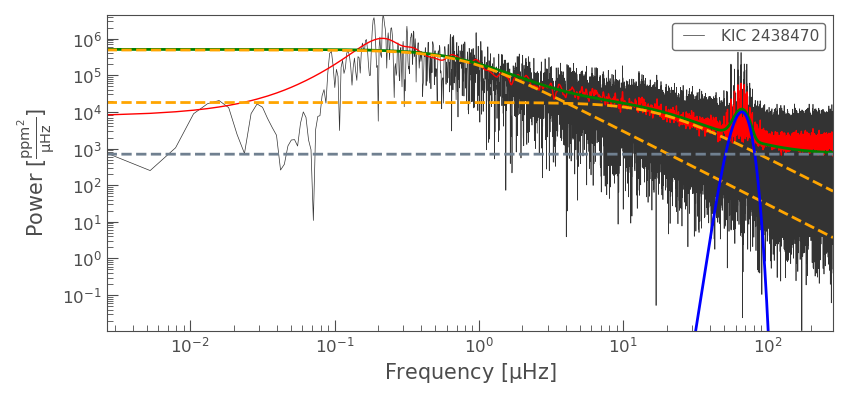
\includegraphics[width=0.99\linewidth]{Chapter5/2438470_ps_harvey.png}
    \caption[Power spectrum of a typical Red Giant solar-like oscillator]{Power spectrum of KIC 2438470, a typical Red Giant solar-like oscillator. A Gaussian-smoothed power spectrum using a $0.1\,\mu$Hz window (red line) is overlaid. The two Harvey components characterising the granulation background (orange dashed lines), a Gaussian fit to the p-mode power excess (blue line) and a constant white noise (grey dotted line) component are overlaid. The total power of the fitted model is also shown (green line).}
    \label{fig:rgps}
\end{figure}

The background convective signal can be effectively described by a Harvey function \citep{harvey_high-resolution_1985}:

\begin{equation}
    P(\nu) = \eta_\mathrm{a}(\nu)^2 \sum_{i} \cfrac{4\sigma_i^2\tau_i}{1+(2\pi\nu\tau_i)^2} + P'_n
    \label{eqtn:Harvey}
\end{equation}

where 

\begin{equation}
    \eta_\mathrm{a}(\nu)^2 = \sinc^2{\left[\cfrac{\pi}{2}\left(\cfrac{\nu}{\nu_{\mathrm{Nyq}}}\right)\right]}
    \label{eqtn:apod}
\end{equation}

\noindent is the apodization factor arising from finite observations, $\sigma_i$ and $\tau_i$ are the amplitude and characteristic timescale of the $i$-th Harvey component \citep{mathur_granulation_2011}, and $P'_n$ is the white noise level. \cite{karoff_observations_2013} and \cite{kallinger_connection_2014} have shown that two Harvey components are sufficient in most cases to describe this background.

The p-mode envelope can be approximately described by a Gaussian \citep{kallinger_evolutionary_2012} and measurements of the modes allows for the extraction of average ``global'' seismic parameters, including:

\begin{itemize}
    \item $\nu_{\mathrm{max}}$ - The frequency at maximum power \citep{kjeldsen_amplitudes_1995, brown_detection_1991}
    \item $\Delta\nu$ - The large frequency separation between radial modes of consecutive order.
    \item $\delta\nu_{nl}$ - The small frequency separations
    \item $\epsilon$ - A phase term dependent on near-surface region properties
\end{itemize}

The frequency at maximum power, $\nu_{\mathrm{max}}$, is linked empirically to the acoustic cutoff frequency, and combined with measurements of the effective temperature, $T_{\mathrm{eff}}$ (eg. from spectroscopy), allows for the direct measurement of surface gravity, $g$, and thus stellar mass and radius:

\begin{equation}
    \nu_{\mathrm{max}} = \cfrac{g}{\sqrt{T_{\mathrm{eff}}}} \;\; \propto \; \cfrac{M}{R^2 \sqrt{T_{\mathrm{Teff}}}}.
\end{equation}

The individual modes that comprise the power excess are regularly spaced in a pattern that is predicted by asymptotic theory \citep{tassoul_asymptotic_1980, gough_solar_1986} with frequencies approximated by:

\begin{equation}
    \nu_{nl} \simeq \left(n +\cfrac{l}{2} + \epsilon \right)\Delta\nu - \delta\nu_{0l},
    \label{eqtn:modes}
\end{equation}
% \begin{equation}
%     \nu_{nl} \simeq \left(n +\cfrac{l}{2} + \epsilon \right)\Delta\nu - \left[Al(l+1)-\delta\right]\cfrac{\Delta\nu^2}{\nu_{nl}}
% \end{equation}

\noindent where $n$ and $l$ are the radial order and angular degree of the specific modes, and $\delta\nu_{0l}$ is a small correction factor that is zero for $l = 0$ modes. The large frequency separation, $\Delta\nu$, is proportional to the sound travel speed across the star and is a direct measure of the mean stellar density \citep{ulrich_determination_1986}.

The phase term, $\epsilon$, is related to the near-surface structure where p-modes are reflected, and is a dimensionless offset of the radial modes typically with a value between 0.5 and 1.5. \cite{christensen-dalsgaard_asymptotic_2014} showed the different locations of the second helium ionisation zone within red clump and red giant branch stars results in different values of $\epsilon$, enabling its use in stellar evolutionary state determinations.

The small frequency separations, $\delta\nu_{02}$ and $\delta\nu_{13}$, depend on the composition of the stellar interior. In main-sequence stars, the low-angular-degree modes probe the core helium content and so are indicators for stellar age \citep{christensen-dalsgaard_introductory_1984, ulrich_determination_1986, christensen-dalsgaard_overview_1988}. In subgiant and red giant stars the turning points of these modes occur before they reach the core. Therefore, in these stars the small frequency separations scale with the large frequency separation instead of probing the evolutionary stage.

The small frequency separation $\delta\nu_{01}$ describes the offset of the dipole modes from the midpoint of the $l = 0$ modes. In main sequence stars, this value probes the stellar core conditions. In red giants, the turning point for the dipole modes occurs at the base of the convective envelope, allowing this small frequency separation to be used as an evolutionary state diagnostic. Typically, red giant branch stars have small, negative values for this separation, whilst in the more evolved red clump stars this offset is positive \citep{montalban_seismic_2010}.

In main-sequence stars, oscillations are purely p-mode in behaviour as g-modes are evanescent in convective regions. For red giants however, all non-radial modes have mixed character with g-mode behaviour in the core and p-mode behaviour in the envelope. This is due to p- and g-modes coupling, resulting in deviations from the regular frequencies of uncoupled modes described by Equation \ref{eqtn:modes} from avoided crossings.

\subsection*{\'Echelle Diagrams}
\label{sect:ech}
\'Echelle diagrams \citep{grec_full-disk_1983} provide a useful diagnostic for displaying and extracting some of these global parameters. Figure \ref{fig:echelle} shows a typical \'echelle diagram for KIC 2438470, constructed by dividing the power spectrum into equal segments of width $\Delta\nu = 6.44\,\mu Hz$, that are then stacked vertically. The $l = 0$ (red circles) and $l = 2$ modes (blue triangles) form roughly vertical ridges, while $l = 1$ modes (black squares) typically show deviations resulting from mixed mode characteristics. All modes are also affected by large-scale stellar structural features that result in curvature of the ridges. To measure the phase shift, $\epsilon$, from an \'echelle diagram, we measure the fractional distance to the $l = 0$ ridge. \cite{huber_asteroseismology_2010} and \cite{white_asteroseismic_2011} have shown $\epsilon$ typically has a value between 0.5 and 1.5, so it may be necessary to add 1 to the resulting fractional distance to get the correct phase shift. The global small frequency separations can also be extracted using this diagram by fitting vertical lines to the centre of the mode ridges and measuring the relevant distances.

\begin{figure}
    \centering
    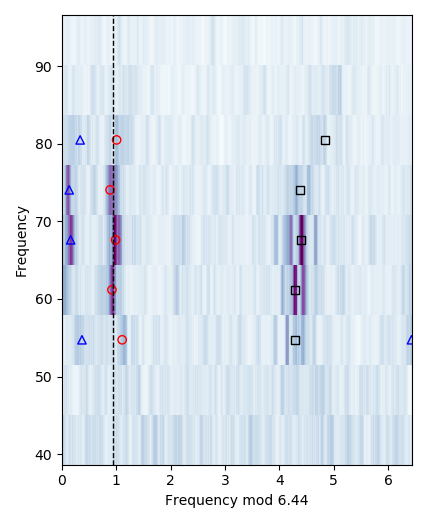
\includegraphics[height=0.5\textheight]{Chapter5/echelle_2438470_somemodes.png}
    \caption[Typical \'echelle diagram for a Red Giant solar-like oscillator]{\`Echelle diagram for KIC\,2438470 with a large frequency separation of $6.44\,\mu\mathrm{Hz}$. The approximate positions of the $l = 0$ modes (red circles), $l = 1$ modes (black squares) and $l = 2$ modes (blue triangles) are plotted. The offset of the $l=0$ ridge due to the phase term, $\epsilon$, at a modulus of 0.929 ($\epsilon = 1.144$) is also highlighted (dashed line). }
    \label{fig:echelle}
\end{figure}

\subsection*{Scaling Relations}

\cite{brown_detection_1991} and \cite{kjeldsen_amplitudes_1995} proposed scaling relations to estimate the global seismic parameters of \numax{} and \dnu{} in solar analogs based on intrinsic stellar properties:

\begin{equation}
    \cfrac{\nu_{\mathrm{max}}}{\nu_{\mathrm{max},\odot}} \simeq \cfrac{M/M_{\odot}\left(T_{\mathrm{eff}}/T_{\mathrm{eff},\odot}\right)^{3.5}}{(L/L_{\odot})}
    \label{eqtn:numax_scaling}
\end{equation}

\begin{equation}
    \cfrac{\Delta\nu}{\Delta\nu_{\odot}} \simeq \cfrac{\left(M/M_{\odot}\right)^{0.5}\left(T_{\mathrm{eff}}/T_{\mathrm{eff},\odot}\right)^{3}}{(L/L_{\odot})^{0.75}} .
    \label{eqtn:deltanu_scaling}
\end{equation}

% \begin{equation}
%     \cfrac{\nu_{\mathrm{max}}}{\nu_{\mathrm{max},\odot}} = \cfrac{M/M_{\odot}}{(R/R_{\odot})^2\sqrt{T_{\mathrm{eff}}/T_{\mathrm{eff},\odot}}}
%     \label{eqtn:numax_scaling}
% \end{equation}

% \begin{equation}
%     \cfrac{\Delta\nu}{\Delta\nu_{\odot}} = \cfrac{(M/M_{\odot})^{1/2}}{(R/R_{\odot})^{-3/2}} 
%     \label{eqtn:deltanu_scaling}
% \end{equation}

\noindent These equations can be rearranged to give the seismic scaling relations:

\begin{equation}
    \cfrac{M}{M_{\odot}} \simeq \left(\cfrac{\nu_{\mathrm{max}}}{\nu_{\mathrm{max},\odot}}\right)^3 \left(\cfrac{\Delta\nu}{\Delta\nu_{\odot}}\right)^{-4}\left(\cfrac{T_{\mathrm{eff}}}{T_{\mathrm{eff},\odot}}\right)^{3/2} ,
    \label{eqtn:mass_scaling}
\end{equation}

\noindent and

\begin{equation}
    \cfrac{R}{R_{\odot}} \simeq \left(\cfrac{\nu_{\mathrm{max}}}{\nu_{\mathrm{max},\odot}}\right)\left(\cfrac{\Delta\nu}{\Delta\nu_{\odot}}\right)^{-2}\left(\cfrac{T_{\mathrm{eff}}}{T_{\mathrm{eff},\odot}}\right)^{1/2} ,
    \label{eqtn:radius_scaling}
\end{equation}


\noindent first used by \cite{stello_oscillating_2008} and \cite{kallinger_asteroseismology_2010} to estimate intrinsic stellar parameters from asteroseismic observations. The value of $\Delta\nu$ in these relations is not directly determined from individual oscillation modes, but rather refers to the gradient of the best-fit linear trend between the radial order (n) and the oscillation frequencies ($\nu_{nl}$). In red giants, the presence of mixed modes beyond the $l = 0$ angular degree restrict this calculation to the radial modes. We note that these scaling relations rely on the assumption the frequencies closely follow the asymptotic relation, which is only true when $n >> l$ and when the stars investigated are essentially homologous to the Sun. In the case of the red giants investigated here these assumptions do not strictly hold true \citep{mosser_asymptotic_2013, belkacem_seismic_2013}, however, some of the deviations introduced as a result of these assumptions effectively cancel out \citep{white_asteroseismology_2013}, and the overall intrinsic stellar properties work out fairly well.

These scaling relations have been extensively applied to the ensemble of asteroseismic observations available from the \textsc{CoRoT}, \Kepler{}, and K2 missions, with many investigations focusing on the accuracy of the estimated intrinsic stellar properties and suggesting small corrections \cite[e.g.][]{basu_determination_2010, white_calculating_2011, miglio_asteroseismology_2012}. For a more detailed summary of these corrections we refer the reader to \cite{hekker_scaling_2020}. 


%
%SCALING RELATIONS!!!!

% The photometric variations in these stars are dominated by surface granulation and the oscillation modes, both of which depend on the surface gravity of the star. 

% Solar-like oscillators
% - global params, echelle diagrams
% Seismic membership (Stello '10, '11)
% Previous red giant results including params, rotation, angle of inclination etc


\section{Cluster light curve processing}
\label{sect:lc_select}

Isabel Colman has produced raw light curves for all cluster members in the 200\,px $\times$ 200\,px \Kepler{} superstamp images of the cluster centres of NGC\,6791 and NGC\,6819 \citep{colman_pixels_2020}. The quality metadata for the superstamp images is generalised to the entire image, providing no localised quality information for a given target. As such, \cite{colman_pixels_2020} made no photometric cuts based on this metadata, and provided no quality flag field for the extracted light curves. The rest of this chapter describes my analysis of these light curves, which were extracted by Isabel using a custom image subtraction code to target stars that I identified in \cref{chap:membership} as likely members (meanprob $\ge 0.03$). Isabel made an additional cut, restricting the standard deviation of the membership score distribution, stdprob, to be stdprob $\leq 0.3$. This cut was made to minimize the chance of extracting foreground and background non-members whose motion and position were not well constrained or coincidentally fell near the edge of the distribution of cluster values. To select the likely red giant members, I made photometric cuts of $G \leq 17.25$ and $G_{BP}-G_{RP}\ge1.25$.

The image subtraction code limits the extraction of data to stars that are at least 2\,pixels from the superstamp edge in a given quarter. As such, stars located close to the image edges may have missing quarters of data in the image-subtracted light curves due to small shifts in the telescope pointing between quarters. These missing quarters tend to fall on the same CCD and result in a regular window function that results in individual oscillation modes being split into clusters of aliased frequencies centred around the actual oscillation frequency. We compared the available image-subtracted data to the \Kepler{} targeted data, and in those cases where additional quarters of data are available, appended the simple aperture photometry (SAP) from the targeted quarters to our image-subtracted light curve. To maintain consistency in terms of quality flags, all data from the SAP light curves was included.

\Kepler{} light curves show a number of instrumental perturbations that must be corrected prior to searching for solar-like oscillations. This is especially important for detecting low-amplitude oscillations. Within single-quarter observations, these perturbations include outliers, discontinuous jumps in the mean observed flux, short-term low-frequency drifts associated early in the mission with instrument temperature changes after safe-mode events \citep{garcia_preparation_2011}, and later with thermal changes during monthly data downlinks, and CCD-specific, quarter-long, low-frequency trends. From quarter to quarter there are also discontinuous jumps and CCD sensitivity changes resulting from the rotation of the \Kepler{} spacecraft. Figure \ref{fig:lc_system} shows examples of these instrumental perturbations. 

\begin{figure}
    \centering
    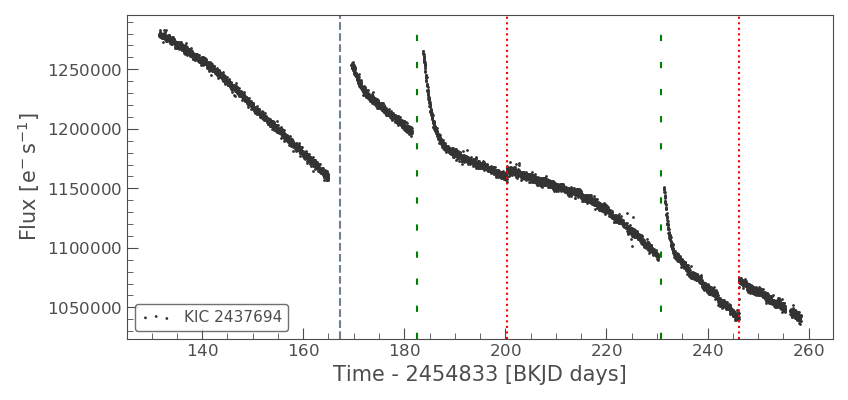
\includegraphics[width=\linewidth]{Chapter5/lc12_systematics.png}
    \caption[Light curve of KIC 2437694 showing quarters 1 and 2]{Light curve of KIC\,2437694 showing quarters 1 and 2. The quarter to quarter CCD sensitivity jump (grey dashes), thermal drifts (green dashes), and discontinuous jumps (red dashes) are shown. Long-term low-frequency trends specific to the CCD can also be seen as general slopes or low-order polynomial trends inherent in each quarter.}
    \label{fig:lc_system}
\end{figure}

Whilst the exoplanet community have developed a number of de-trending algorithms to correct \Kepler{} systematics, these tools have been designed to search for transits that are typically small-amplitude periodic signals are localised in time. In contrast, stellar oscillations are present throughout the entire time series of the light curve in essentially stable modes. In particular, the thermal ramping effects and consequent changes in statistical noise characteristics in the first 2-3\,days of data following downlinks are challenging to overcome for exoplanet searches and are typically removed. However, introducing larger gaps in the time series (beyond the downlink gap), results in an increased window function within the Fourier transform typically used to analyse asteroseismic signals. This decreases the sensitivity of searches for solar-like oscillations, particularly for those in the higher-frequency and lower-power regime (less evolved solar-like oscillators). For asteroseismic analyses, large discontinuous changes in flux must be corrected for as they generate power at many frequencies, but changes in noise properties from one segment to another are less of an issue, provided they are not too severe.

\subsection{Correction Methods}

We investigated three different correction processes to remove instrumental perturbations within each quarter: high-pass filtering using a custom Gaussian filter, polynomial de-trending, and Co-trending Basis Vectors (CBVs). We initially corrected all of our extracted light curves with a simple Gaussian high-pass filter designed to account for the irregularly sampled data with missing data points. We applied this filter on a quarter by quarter basis to each light curve with window widths equivalent to 0.5\,d, 1\,d, and 2\,d standard deviation Gaussians. This process is sufficient for stars with high frequency variations but removes all low-frequency trends, including the oscillation power excesses of red giants with \numax{} lower than about 15\,$\micro$Hz. It also affects the extraction of the granulation signal parameters for these stars.

To minimize over-fitting in our light curve corrections, and to try to retain more of the low-frequency oscillation and granulation signals, we next investigated high-pass filtering with low-order polynomials. These low-frequency trends can be treated as polynomial trends of relevant order that can be fitted and divided out. To automate this process, we implemented a 5-fold cross-validated linear regression to select the optimum polynomial order to fit each quarter. Cross validation refers to machine learning techniques used for determining the optimal model to apply to a data set. These techniques are typically based around dividing an input data set into smaller subsets that are tested and then compared, to determine how well the model fit will generalise to the full data set \citep{mosteller1965data}.

In this case, we divided our light curve data into two sets: a training set, used by the fitting routine to obtain the polynomial coefficients of our model, and a validation set, that is not used in the polynomial fit but is used to test how well the model fits unseen data. We selected a split of 70\% training data to 30\% validation data for this work, as this provides a large sample size for both model fitting and validation. We then selected models with polynomial orders of 1 to 6 and, for each order, calculated a mean-squared-error metric for the validation set. To eliminate the possibility of selection bias in our random split of the light curve data we repeated this process for 5 different `folds' or splits. We then select the order that has the best overall fit to the validation data sets. This is the order that has the best metric value when averaged across the combined validation sets. We have found that polynomial de-trending works well in cases where the stars have a strong low-frequency trend and no discontinuities or thermal slopes in the light curve. This is not the case for most quarters of \Kepler{} data, and resulted in poor polynomial fits and over-corrections, most notably in the photometry from the CCD that NGC\,6791 fell on for quarters 2, 6, 10 and 14. In addition, the \Kepler{} systematics are not well-described as simply a combination of low-frequency trends, as polynomial de-trending accounts for, but include trends at higher frequencies as well that remain uncorrected in the resulting light curves. %The polynomial fit also resulted in difficulties in producing well-aligned quarter-to-quarter stitched light curves.  

\subsubsection{Correction with Co-trending Basis Vectors}

After trying these two simpler correction methods, we describe a more sophisticated correction routine, which aims to minimize over-fitting and retain as much of the intrinsic variability as possible. As part of this work, we implemented a custom Principle Component Analysis (PCA) of different ensembles of light curves to produce Co-trending Basis Vectors (CBVs). PCA is a method of dimensionality reduction that creates new features or components from linear combinations of the original features in the data. These principle components, or basis vectors, present the axes of greatest variance \citep{jolliffe_principal_2016}, and are ranked from highest to lowest variance. In this case, we are referring to a set of uncorrelated features present in the ensemble of light curves that represent the systematic trends we wish to remove. 

We corrected our light curves with three different basis vectors: (a) the default \Kepler{} CBVs, (b) custom CBVs based on the full sample of image subtraction extracted member stars, and (c) custom CBVs based on the subset of stars identified as likely red giant members.

We began our CBV corrections using the default \Kepler{} CBVs that comprise the 16 most significant CBVs for each quarter based on the targeted stars within each CCD channel \citep{thompson_kepler_2016}. The \texttt{lightkurve} python package \footnote{https://docs.lightkurve.org/} provides a linear least-squares minimisation routine to correct targeted light curves, which it stores as \texttt{KeplerLightCurve} objects\footnote[2]{`Objects' here refers to the programming concept of a data structure that contains different attributes or properties, such as times and fluxes, and code in the form of methods that can be applied to these objects.}, using these basis vectors. By default, this package uses the 2 highest-order CBVs to fit and remove systematic signals, whilst avoiding significant over-fitting of intrinsic stellar variability. We produced \texttt{KeplerLightCurve} objects for each extracted red giant, which are able to be used with the \texttt{lightkurve} reduction methods and which enabled us to apply this CBV correction routine.

We found that our image-subtracted light curves exhibited differences in their systematic trends compared to the light curves extracted using the targeted simple aperture photometry. To account for these differences, we produced two sets of custom CBVs using the \texttt{scikit-learn} python package:
\begin{itemize}
    \item For the first set of custom CBVs we derived CBVs from the complete set of image-subtracted light curves for each superstamp. Figure \ref{fig:cbvs_allIS_Q1} shows the first 8 CBVs for the first data quarter of NGC\,6791, and the Fourier transforms of these basis vectors.
    
    \item For the second custom CBV set we derived CBVs from the subset of image-subtracted light curves corresponding to only the likely red giant members in each cluster. Figure \ref{fig:cbvs_rgsubset_Q1} shows the corresponding CBVs and Fourier transforms for this subset in NGC\,6791.
\end{itemize}

\begin{figure}
    \centering
    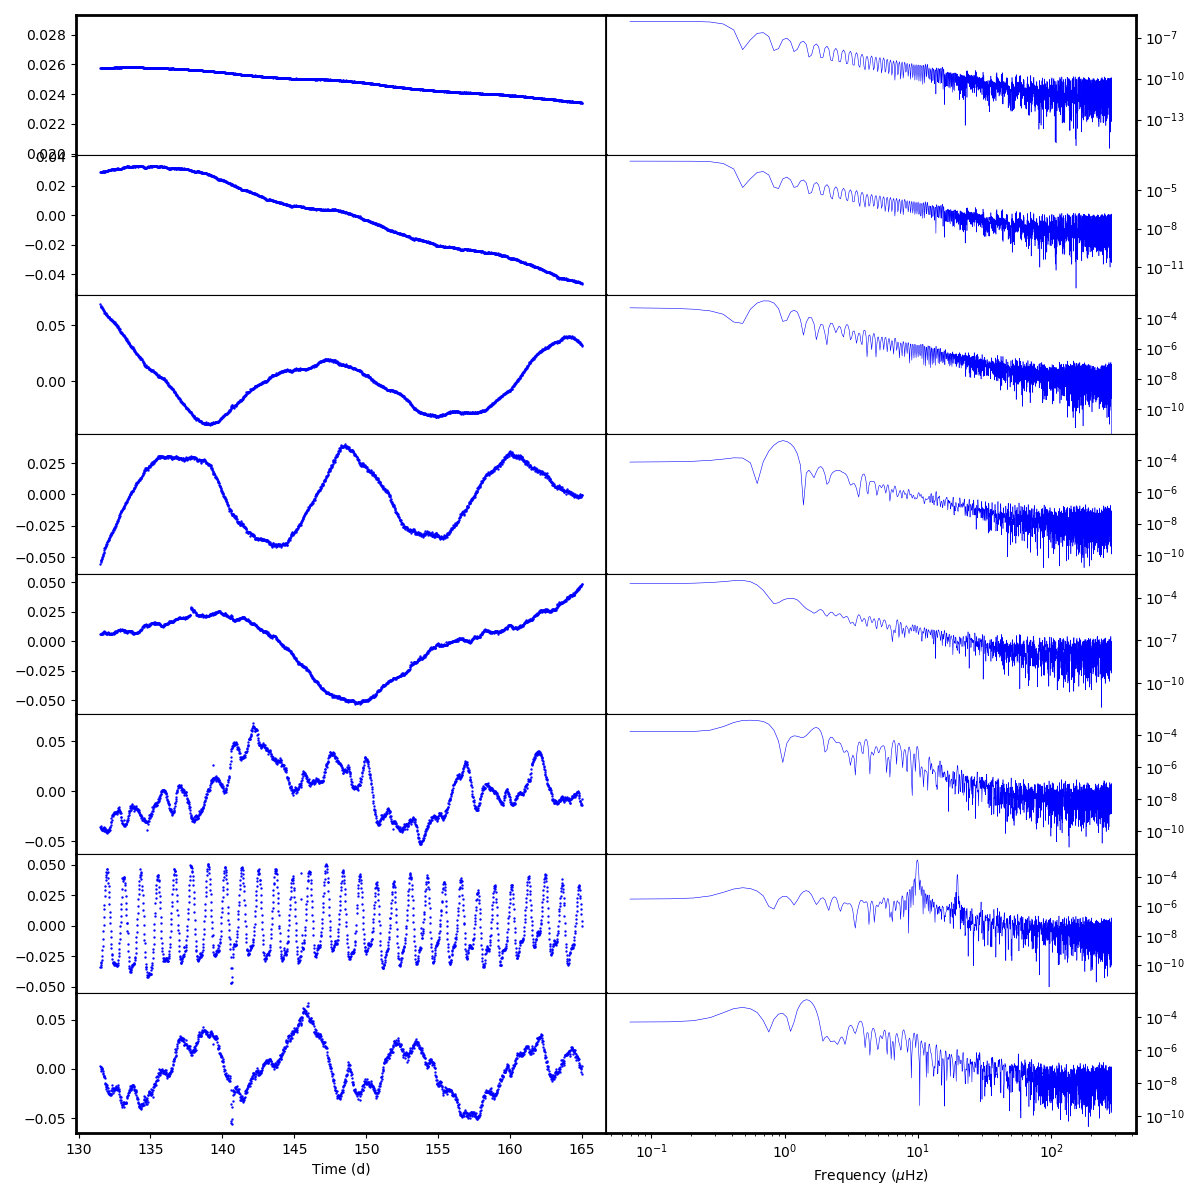
\includegraphics[width=\linewidth]{Chapter5/cbv_6791_q01.png}
    \caption[Custom co-trending basis vectors with Fourier transforms (I) Full image-subtracted subset]{The first 8 co-trending basis vectors (CBVs) for NGC\,6791 for the first data quarter (left), and the Fourier transform of these vectors in log-log space (right) from the full set of image-subtracted light curves.}
    \label{fig:cbvs_allIS_Q1}
\end{figure}

\begin{figure}
    \centering
    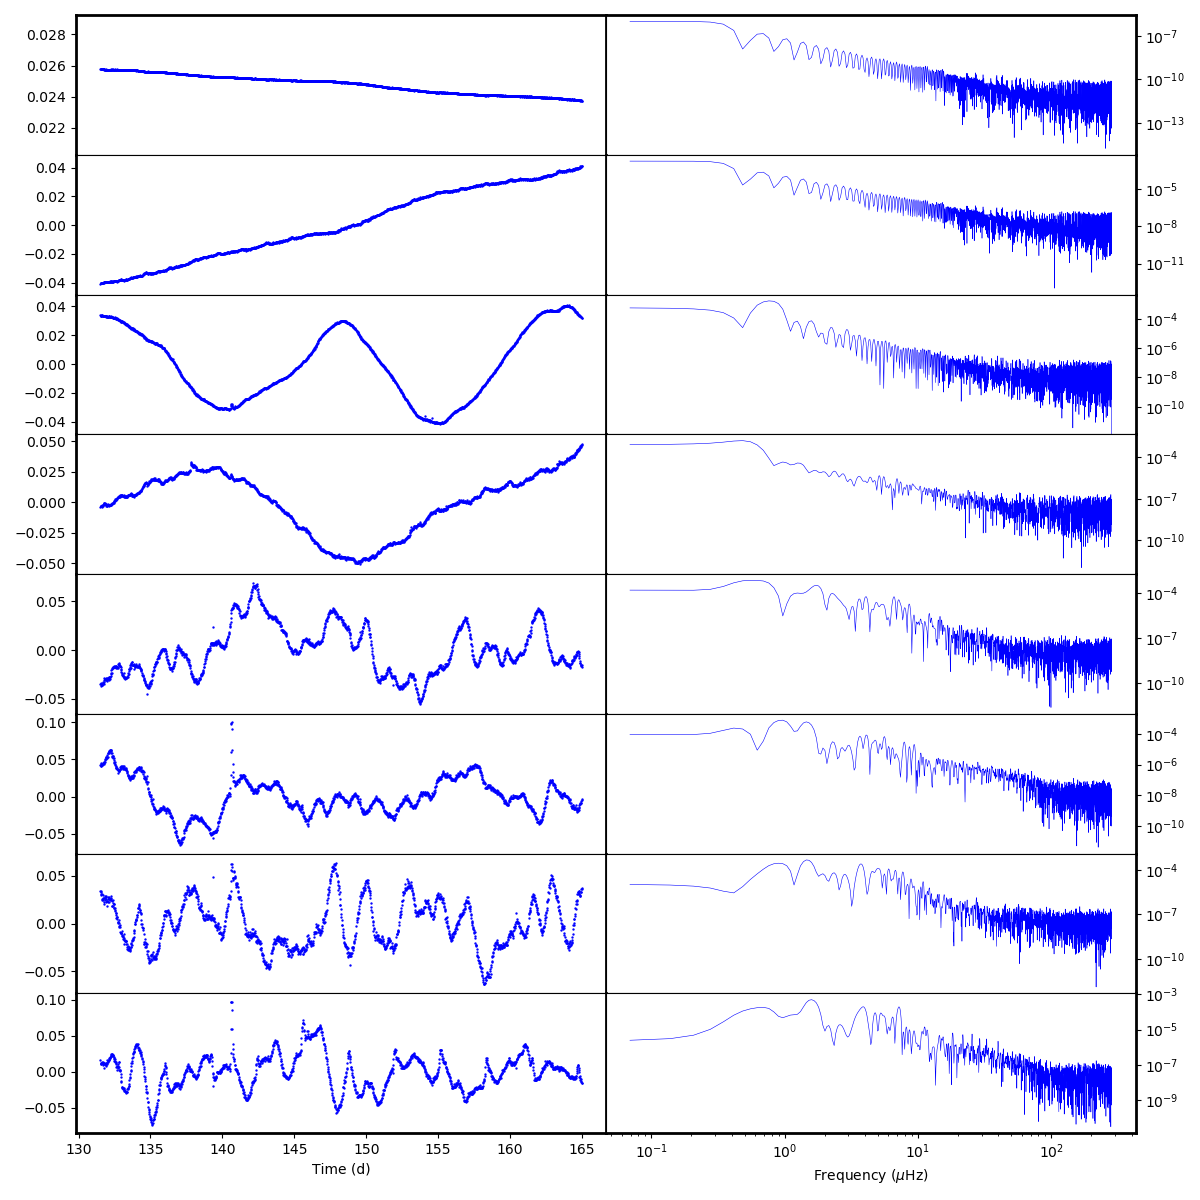
\includegraphics[width=\linewidth]{Chapter5/cbv_6791_rgs_q01.png}
    \caption[Custom co-trending basis vectors with Fourier transforms (II) Red Giant subset]{Same as Figure \ref{fig:cbvs_allIS_Q1} but for the likely red giant member subset of NGC\,6791.}
    \label{fig:cbvs_rgsubset_Q1}
\end{figure}

We implemented a manual correction process that enabled a selected number of CBVs to be applied, based on a least-squares minimisation routine satisfying:

\begin{equation}
    \mathrm{LC}_{\mathrm{corr,n}} = \mathrm{LC}_\mathrm{raw} - \sum_{i=1}^{n} \left(A*\mathrm{CBV}_i + B\right) .
    \label{eqtn:mini}
\end{equation}

\noindent We further designed an automated selection routine that iteratively increased the number of applied CBVs, up to a maximum of 8 vectors, and selected the first corrected light curve where the variance was lower than twice the smallest variance. These selected light curves corrected for the instrumental perturbations, yet retained stellar variability for oscillations above a frequency of about 1\,$\mu$Hz. Figure \ref{fig:cbv_eg_q1} shows the effect of iteratively applying the red giant CBVs to the quarter 1 light curve for KIC\,2436900 in NGC\,6791. We offset the corrected light curves for clarity. We can see that the first CBV removes the predominant low-frequency trend in the light curve (blue to orange), with the application of 3 CBVs correcting for most of the low-frequency variability whilst still retaining the red giant power excess around 30$\mu$Hz, as well as the granulation signal down to a frequency of approximately 3$\mu$Hz. 

\begin{figure}
    \centering
    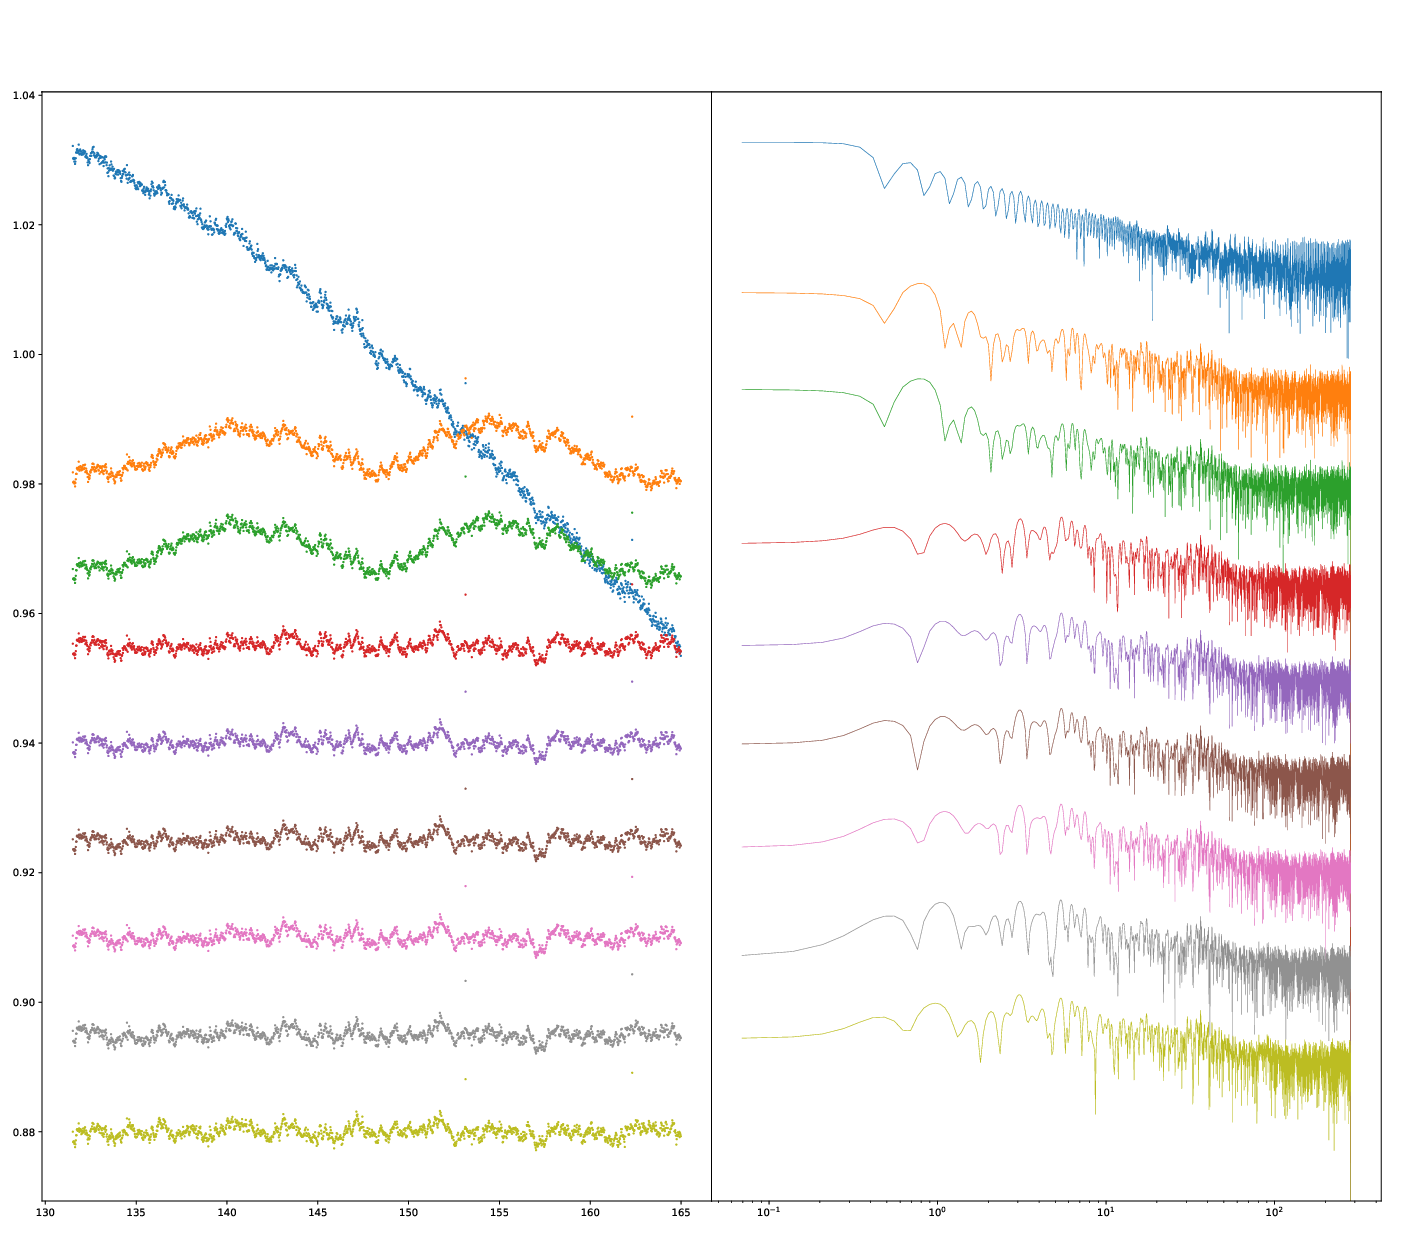
\includegraphics[width=\linewidth]{Chapter5/KIC_2436900_detrending_CBVs_q01_rgs_lsq_mod2.png}
    \caption[Correction effect of applying an increasing number of RG-subset-derived CBVs to a typical RG light curve]{The light curves (left) and power spectra (right) for KIC 2436900 beginning with the raw image-subtracted data (blue), and with increasing orders of applied basis vectors (orange through mustard). The corrected light curves are offset for clarity. Typically, the red corrected light curve would be selected.}
    \label{fig:cbv_eg_q1}
\end{figure}

\subsubsection{Interpolating missing observations}
Further complicating the investigation of low-amplitude oscillations is the window function of the observations \citep{garcia_impact_2014}. Figure \ref{fig:window_function} shows the effect of these time gaps on the spectral window, calculated for a 1\,$\mu$Hz signal with an amplitude of 1\,ppm. The spectral window for the extracted light curves (black) has a very high background level, particularly above 25-30\,$\mu$Hz, due to the introduction of side-lobes of the low-frequency signal at higher frequencies. One of the main causes was \Kepler's angular momentum dumps, which occurred every $\sim3$\,days and resulted in regular gaps of a single long-cadence data point.

\begin{figure}
    \centering
    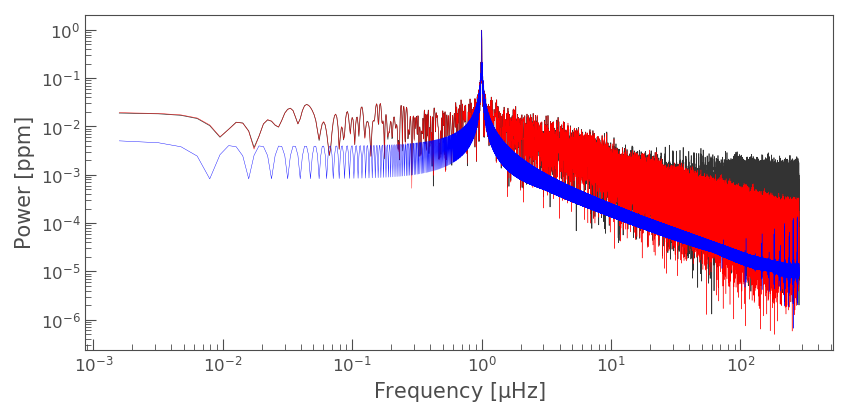
\includegraphics[width=\linewidth]{Chapter5/window_function_example1uHz1ppm.png}
    \caption[Power spectral window, showing the effect of the \Kepler{} window function]{Power spectral window, showing the effect of the \Kepler{} window function on a 1\,ppm 1\,$\mu$Hz signal. The spectral window for the extracted light curves (black line) has a very high background level compared to the same signal observed with the momentum dump gaps interpolated (red signal). For comparison, we have included the power spectrum of the signal observed at a regular cadence with no gaps for the entire \Kepler{} mission (blue line).}
    \label{fig:window_function}
\end{figure}

This spectral window particularly affects the frequency ranges that fainter red giant cluster members oscillate within. To minimize this effect, we interpolated the missing observations from the angular momentum dumps. To interpolate these points we implemented a 5-Fold cross-validated k-Nearest Neighbour (kNN) regression algorithm. The k-Nearest Neighbour algorithm is a simple non-parametric algorithm that selects the `k' data points that are closest to the missing data point in the parameter space, in our case time, and uses the values of these points to predict the missing value. We allow the value of k to vary between 1 and 30 data points for the interpolation, and once again selected our cross-validation sets, to prevent over-fitting, at a 70:30 ratio of training to validation data, with 5 folds. We found that this algorithm almost always selected the 3 closest data points (k=3) to conduct the mean interpolation of flux values for the missing angular momentum dump observations.

Finally, we implemented custom scaling and stitching methods to correct for the quarter to quarter CCD sensitivity differences. Figure \ref{fig:correction_process} presents a summary chart of the correction processes we implemented.

\begin{figure}
    \centering
    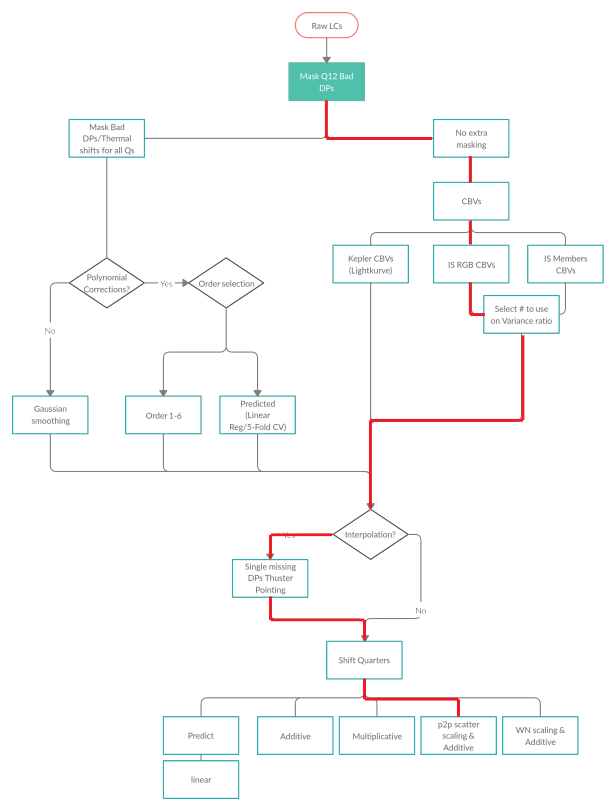
\includegraphics[width=\linewidth]{Chapter5/correction_process.png}
    \caption[Correction process routines]{Flow diagram showing the different correction processes applied to each light curve. The final selected light curve correction routine is highlighted (red line).}
    \label{fig:correction_process}
\end{figure}

\section{Application of Correction methods}

We tested the correction processes on 10 red giants with targeted \Kepler{} light curves of equal length to our image-subtracted light curves. The equal length of observations make these stars ideal test cases. The correction process resulted in over 1\,000 `corrected' light curves with a processing time greater than 15\,minutes per star. These light curves included manual and automated selection of: the number of CBVs applied (to a maximum of 8), and the polynomial order (from 1st order to 6th order corrections), as well as the application of Gaussian high-pass filtering with 0.5\,d, 1\,d and 2\,d kernel widths.

The resulting light curves were then optionally interpolated to fill the single missing observations corresponding to angular momentum dumps. Finally, we stitched the individual quarters together using either an additive or multiplicative flux shift to align the quarters. In the case of the additive flux shift, we also included the option of multiplicative scaling of these quarters based on the point-to-point (p2p) variance, standard deviation, or Lomb-Scargle periodogram white noise amplitude of each quarter.

To speed up the correction process, we processed 10 \Kepler{} targeted red giants with known $\nu_\mathrm{max}$ values and, for each star, manually compared the white noise amplitude and low frequency profiles for our 20 corrected image-subtracted light curves that had the highest signal-to-noise. The automated custom CBVs correction based on the red giant branch subset consistently returned high signal-to-noise ratios of the power excess, as well as retaining more power at low frequencies than Gaussian high-pass filtering. 

For all subsequent red giant light curve corrections, we selected our custom red giant CBV correction routine, interpolated missing points in each quarter using our kNN interpolation method, and finally stitched the resulting light curve quarters with our p2p-scaled additive quarter shift routine. We have marked this process in red in Figure \ref{fig:correction_process}.

We also note that the extracted light curves had a large number of outliers in quarter 12, resulting from coronal mass ejection impacts with \Kepler{} \citep{van_cleve_kepler_2016}, that we removed prior to any other corrections being applied. In the case of those red giants that have a mixture of image-subtracted photometry and simple aperture photometry, we could not assume that our custom CBVs derived from the red-giant subset would accurately correct the systematic perturbations. As such, we only applied a 0.5\,d Gaussian high-pass filter in these cases, to remove the low-frequency trends from each light curve quarter, and then stitched the resulting corrected light curves with our custom p2p-scaled additive shift method.

\subsection{Superstamp times}

During our correction process, we found a small sinusoidal time shift between targeted stars (as downloaded from MAST) and their superstamp light curves (e.g. Figure \ref{fig:keptimediff}). We measured this time shift to have a maximum amplitude of $\sim1.30$\,s for KIC\,2436900 and $\sim1.21$\,s for KIC\,2570924, which are on opposite sides of the superstamp. We attribute this shift to the correction of the observation times to Barycentric Julian Date (BJD). This correction depends on the ecliptic latitude of the specific star, so it varies across the superstamps. For targeted stars these corrections were made individually for each star, but for the superstamps a single correction per cadence was made. We have found that this time shift decreases in amplitude as we move closer to the centre of the \Kepler{} FoV, and infer that these corrections are based on a reference point at its centre. We note this trend for completeness, but due to its negligible effect on our analysis we did not correct for it.

\begin{figure}[h]
    \centering
    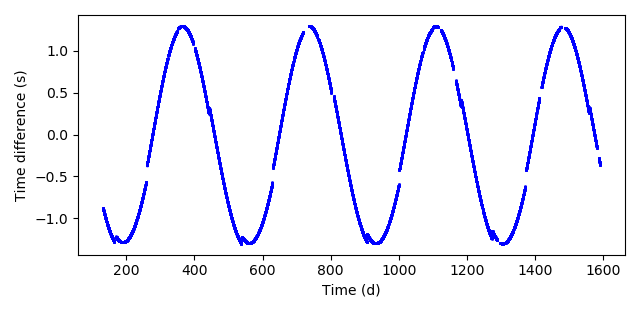
\includegraphics[width=\linewidth]{Chapter5/kepler_time_diff.png}
    \caption[Superstamp and targeted light curve time difference]{Calculated time difference between cadences of the superstamp and targeted light curve for KIC\,2436900.}
    \label{fig:keptimediff}
\end{figure}

\section{Individual results}

We manually reviewed each likely red giant member during our analysis and have identified: 

(a) new red giant members for both NGC\,6791 and NGC\,6819,

(b) rotational modulation in either foreground red dwarfs or background giants, and 

(c) 2 other variable stars. 

Figures \ref{fig:cmd_new} and \ref{fig:cmd_newz} show the CMD for NGC\,6791, based on the likely members from Chapter \ref{chap:membership}, focused on the red giant branch, with the locations of our identified variables marked. Figure \ref{fig:cmd_new_2} shows the same for NGC\,6819.

\begin{figure}
    \centering
    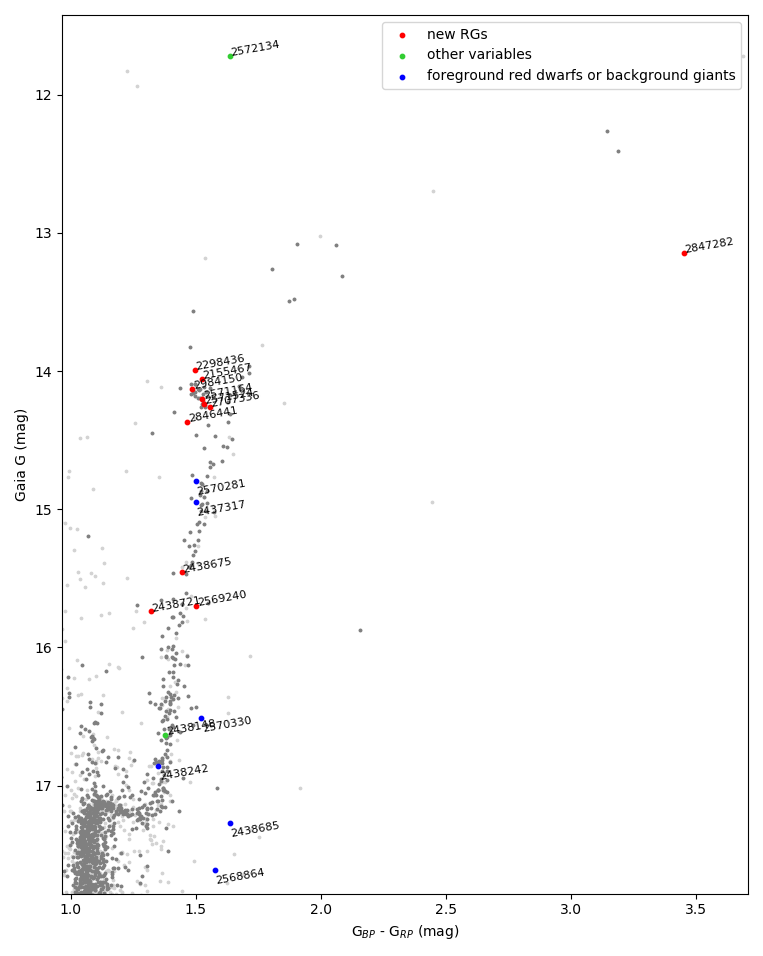
\includegraphics[width=\linewidth]{Chapter5/6791_CMD.png}
    \caption[CMD of new variables in the RG branch in NGC 6791]{CMD of the RG branch in NGC\,6791 with RGs we have identified oscillations in for the first time (red), along with foreground rotational variables (blue), and other interesting variables (green). All likely cluster members (light grey) and the subset of these falling on the \Kepler{} superstamps (dark grey) are shown.}
    \label{fig:cmd_new}
\end{figure}

\begin{figure}
    \centering
    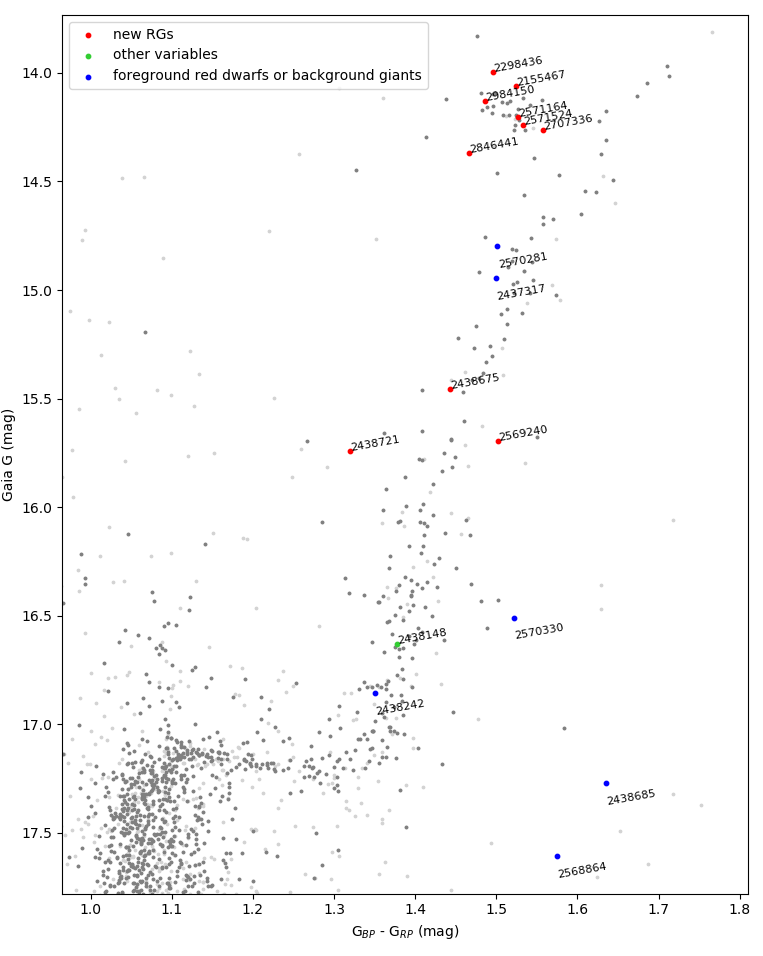
\includegraphics[width=\linewidth]{Chapter5/6791_CMD_zoom.png}
    \caption[NGC\,6791 CMD zoom]{Same as Figure \ref{fig:cmd_new}, zoomed into the crowded region of the RGB.}
    \label{fig:cmd_newz}
\end{figure}


\begin{figure}
    \centering
    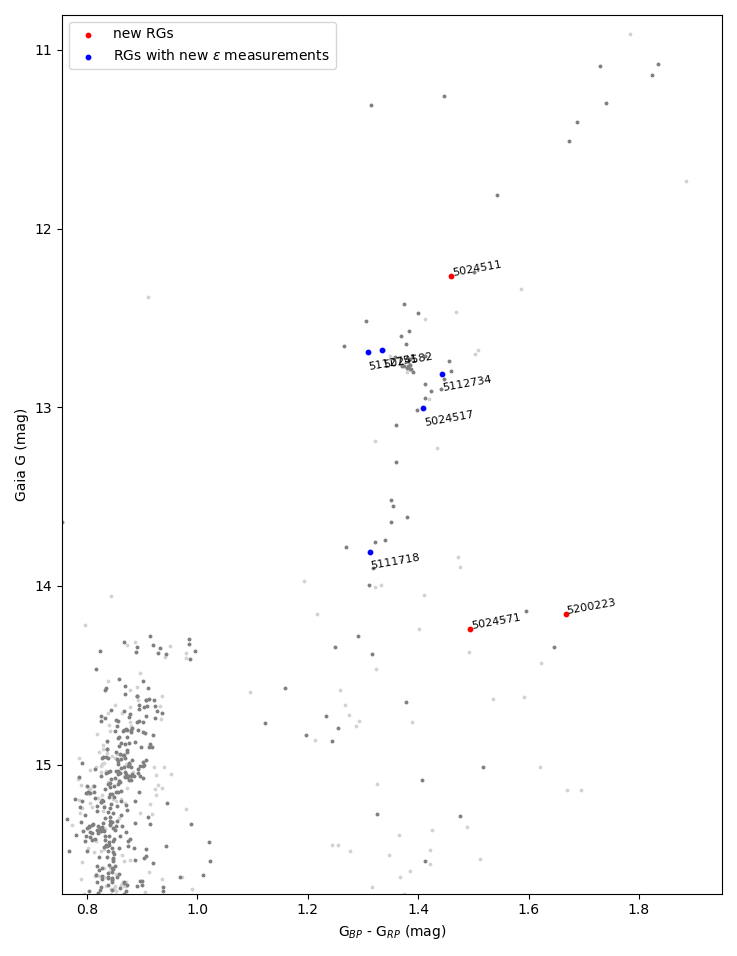
\includegraphics[width=\linewidth]{Chapter5/6819_CMD_newRGS_interesting.png}
    \caption[CMD of new variables in the RG branch in NGC 6819]{CMD of the RG branch in NGC\,6819 with RGs we have identified oscillations in for the first time (red), along with those red giants where we have extracted values for $\epsilon$ for the first time (blue).}
    \label{fig:cmd_new_2}
\end{figure}

\subsection{KIC 2847282}

Figure \ref{fig:2847282_lc} shows the light curve for KIC\,2847282, an M-giant cluster member in NGC\,6791 whose oscillations have not previously been examined in detail. This star does not fall on the \Kepler{} superstamps but was targeted for quarters 10 through 14. In our identification of stellar oscillations in this star we used the \Kepler{} Pre-search Data Conditioning SAP (PDCSAP) \citep{smith_kepler_2012}, a modified version of the simple aperture photometry mentioned in Section \ref{sect:lc_select}, that has been corrected for artefacts such as instrumental systematics. \cite{yu_asteroseismology_2020} included KIC\,2847282 in their ensemble investigation of \Kepler{} long-period variables, noting a period of 27.74\,days but did not identify it as a member of NGC\,6791.

Identification of the centre of the power excess, \numax{}, is difficult in such stars; instead the focus is to identify the individual modes. The power spectrum of KIC\,2847282 is shown in Figure \ref{fig:2847282_ps} (lower panel), with vertical lines marking what are potentially individual oscillation modes, or unresolved groups of modes (one group per radial mode order). These vertical lines connect with the ensemble power spectra from \cite{yu_asteroseismology_2020} (top). We show three potential mode identifications (horizontal lines) based on a cross match between the two plots. Based on the amplitudes, we selected the \numax{} value of 0.68\,$\mu$Hz as corresponding to the most likely mode identifications, with the highest peak corresponding to an order of $n = 2$, with peaks matching up to an order of $n = 5$. We note that the mode identifications corresponding to \numax{} values of $\sim$\,0.41\,$\mu$Hz and $\sim$\,1.0\,$\mu$Hz remain as alternative identifications. This result identifies KIC\,2847282 as the third most luminous red giant in NGC\,6791 and a good candidate for detailed asteroseismic modelling. Whilst we classify this star as a member of NGC\,6791, based on the high membership score (0.72, where any value greater than 0.03 is a likely member), the position of this star in the CMD is unusual for a cluster member, so the possibility exists that this may be a background giant.

\begin{figure}
    \centering
    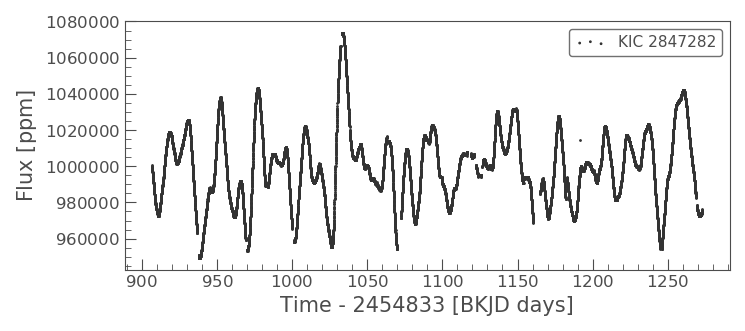
\includegraphics[width=\linewidth]{Chapter5/2847282_MGiant_lc.png}
    \caption[PDCSAP light curve for the new M-giant, KIC\,2847282]{PDCSAP light curve for KIC\,2847282. This is a newly identified M-giant cluster member in NGC\,6791 that does not fall on the superstamps but was targeted for quarters 10 through 14.}
    \label{fig:2847282_lc}
\end{figure}

\begin{figure}
    \centering
    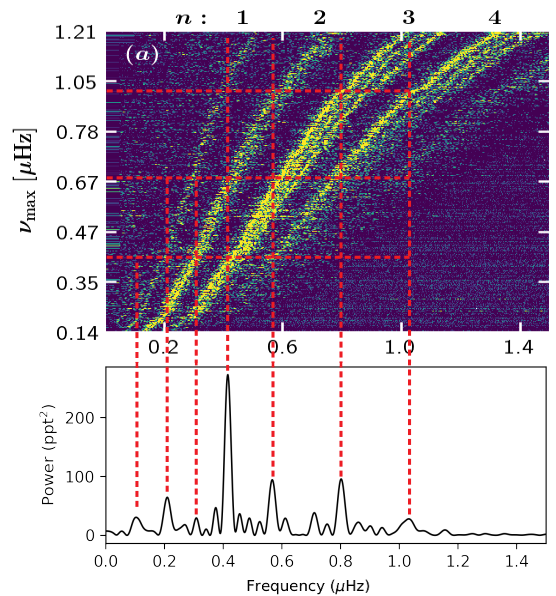
\includegraphics[width=0.6\linewidth]{Chapter5/mode_id_MG.png}
    \caption[Power spectra with possible mode identifications for KIC\,2847282]{Power spectra for KIC\,2847282 (bottom) with three potential values of \numax{} (horizontal lines) based on a cross match between the power spectrum peaks and the ensemble power spectrum trends (top) from \cite{yu_asteroseismology_2020}. The middle line corresponds to our most likely choice of \numax{}$\sim$0.68\,$\mu$Hz, with the highest peak corresponding to an order of n=2, and peak matches up to an order of n=5. The remaining horizontal lines correspond to alternative identifications of \numax{}$\sim$0.41\,$\mu$Hz and \numax{}$\sim$1.0\,$\mu$Hz.}
    \label{fig:2847282_ps}
\end{figure}

\subsection{KIC 5024517}

Figure \ref{fig:5024517_ps} shows the power spectrum for KIC\,5024517, a \Kepler{} target star in NGC\,6819 for which we identify a potential RG\textendash{}RG binary power excess for the first time, centred around $\sim$22$\mu$Hz and $\sim$50$\mu$Hz. It is rare to see a light curve in which oscillations from two red giants are visible. This star was included in \citet{bellamy_using_2015} but only the $\sim$50$\mu$Hz power excess was measured. The decreasing amplitudes of the power excesses with increasing frequency is consistent with two co-distant red giants, with the most likely explanation being that this is a newly identified RG\textendash{}RG binary system. An alternative explanation is this is a blend of two cluster red giants that are located close to each other on the sky. To determine probabilities of red giant line-of-sight blends within the 4” of the Kepler pixels, \citet{colman_pixels_2020} used GALAXIA simulations \citep{sharma_galaxia_2011} to generate artificial populations of stars within a synthesised Kepler FoV. They calculated the occurrence of such alignments to be rare, with a probability of less than 11\%. This occurrence was for a blend between a red giant and any other star. The chance of having two red giants aligned within this distance cutoff is smaller still, although the crowded nature of the cluster means we cannot rule out this possibility without further data. Radial velocity measurements could potentially confirm the possibility of an RG\textendash{}RG binary based on mass ratios if such a system exists.

\begin{figure}
    \centering
    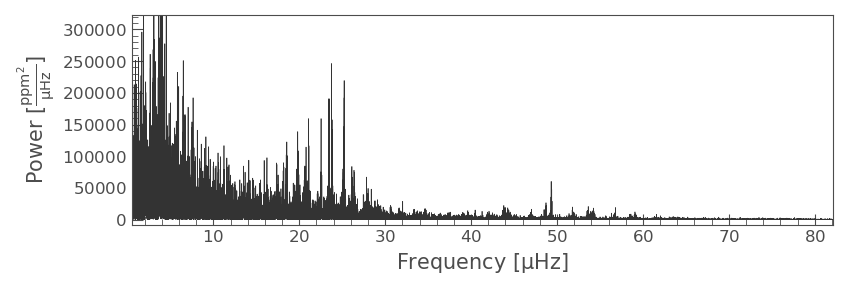
\includegraphics[width=\linewidth]{Chapter5/5024517_ps.png}
    \caption[Power spectrum of the new potential RG\textendash{}RG binary, KIC\,5024517]{Power spectrum of KIC\,5024517, a new potential RG\textendash{}RG binary in NGC\,6819.}
    \label{fig:5024517_ps}
\end{figure}

\subsection{Rotationally-modulated variable stars}

In the course of this work, we re-classified 6 stars in NGC\,6791 from likely red giant members based on our photometric cuts and GMM membership (Chapter \ref{chap:membership}), to either foreground red dwarfs or background giants. Our uncertainty in determining the nature of these stars as either foreground or background stars is due to the unconstrained {\em Gaia} parallax values for each star, with the uncertainty on these values being on order of the value itself. We flagged two of these stars in NGC\,6791, KIC\,2568864 and KIC\,2438685, because their locations in the CMD (Figure \ref{fig:cmd_new}) were too far to the red to be cluster red giants. We inspected their light curves and noted the presence of rotational modulation. Rotational modulation is caused by star spots, providing cooler (and thus dimmer) surface areas that reduce the overall stellar flux, coupled with the stellar rotation period. Such stellar spots in main sequence stars are typically limited in size and change quickly over the timespan of these observations. These light curves are typical of red giants or red dwarf stars, exhibiting stellar flares and rotational modulation. The presence of rotational modulation coupled with the lack of detectable oscillations in the Fourier transforms, and combined with effective temperatures of 4409\,K and 4248\,K, respectively, place these stars as likely foreground red dwarfs, rather than cluster red giants.

The remaining four re-classified stars all fall close to the red giant branch, and for all four we found rotational modulation in their light curves. We note that KIC\,2437317 was previously classified by \cite{bellamy_new_2015} as an M-giant in his Master's thesis \citep{bellamy_using_2015}, however, inspection of the light curve reveals rotational modulation, and the power spectrum shows a resolved peak around 0.31\,$\mu$Hz with a harmonic around 0.62\,$\mu$Hz. In addition, flares are visible in the light curves for KIC\,2437317, around 841.2 and 843.9\,days, and in KIC\,2438242, around 899.3\,days, confirming these stars as M-dwarfs. Figure \ref{fig:reddwarfs} shows the rotational modulation signal evident in the uncorrected quarter 8 and quarter 9 image-subtracted light curves for these stars. The light curves for quarter 9 have been shifted vertically to enable easier comparison of the rotational signal from one quarter to the next. Where possible we measured the rotational periods of these stars using the \texttt{Exoplanet} Gaussian Process code with a simple rotational kernel following the process described in \cite{foreman-mackey_fast_2017}. Table \ref{tab:reclassified} lists the KIC IDs, effective temperatures, alternative ID's from previous photometric studies, and the rotational periods we were able to measured for these reclassified stars. By combining our investigation of the \Kepler{} light curves with our astrometric membership, we were able to improve our cluster membership identifications by removing foreground or background stars that would otherwise have been classified as likely members.

\begin{figure}
    \centering
    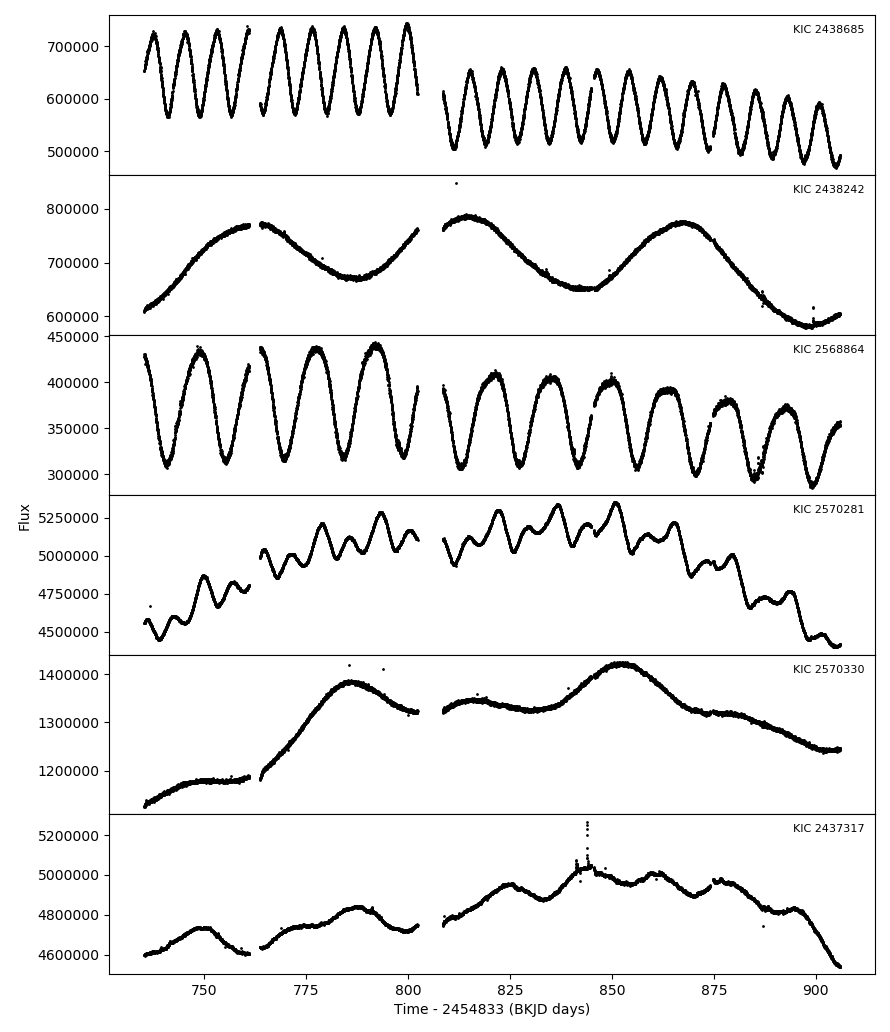
\includegraphics[height=\linewidth]{Chapter5/Rot_mod_5_q89.png}
    \caption[Light curves for 6 re-classified foreground red dwarfs or background giants in NGC 6791]{Light curves for the 6 re-classified foreground red dwarfs or background giants in NGC\,6791, showing characteristic rotational modulation from star spots. KIC\,2437317 shows evidence for flares around 841.2 and 843.9\,days, while KIC\,2438242 shows a potential flare around 899.3\,days. The presence of flares would confirm these stars as M-dwarfs.}
    \label{fig:reddwarfs}
\end{figure}

\begin{table}
    % \centering
    \begin{tabular}{ccccc}
        KIC ID  &   Alternative   & $T_\mathrm{eff}$  & Rotational  & Classification \\%& Reference \\
                &       ID           &    (K)            & Period (d)  &                \\ \hline%& \\ \hline
        2438685 &   \textendash      &  4248             &     7.78    &  \textendash       \\
        2438242 &   V710 Lyr         &  4722             &    54.1     &  M-dwarf \\
        2568864 &   01431\_10        &  4409             &    14.2     &  \textendash       \\%& None\\
        2570281 &   V692 Lyr         &  4643             &    14.5     &  \textendash      \\
        2570330 &   V630 Lyr         &  4609             &    67.7     &  \textendash       \\%& None\\
        2437317 &   V566 Lyr         &  4250             &    17.6     &  M-dwarf     \\

    \end{tabular}
    \caption{Stars re-classified as foreground or background rotational variables}
    \label{tab:reclassified}
\end{table}

\subsection{Other variables}

During inspection of each likely red giant member we identified two other variables in NGC\,6791.  We present the light curves and power spectra for these stars in Figure \ref{fig:weirdvars}. KIC\,2572134 appears to be an irregular variable with a \numax{} around $\sim$6.6\,$\mu$Hz, but it is too blue to be a cluster member unless it is an evolved blue straggler. KIC\,2438148 has a pulsation spectrum that looks typical for a single-mode $\delta$ Scuti variable, but its KIC effective temperature of 4906\,K and colour, $B - V \simeq 1.18$, are too cool for this interpretation. Further investigation, such as obtaining a spectrum, is needed to clarify the variable classification for this star.

\begin{figure}
    \centering
    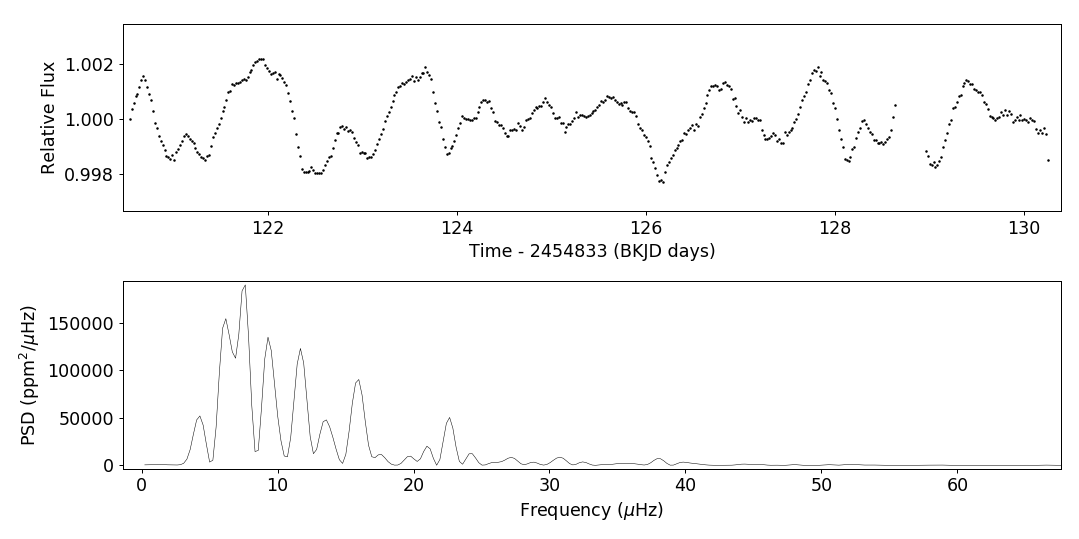
\includegraphics[width=0.9\linewidth]{Chapter5/2572134_lc_ps.png}
    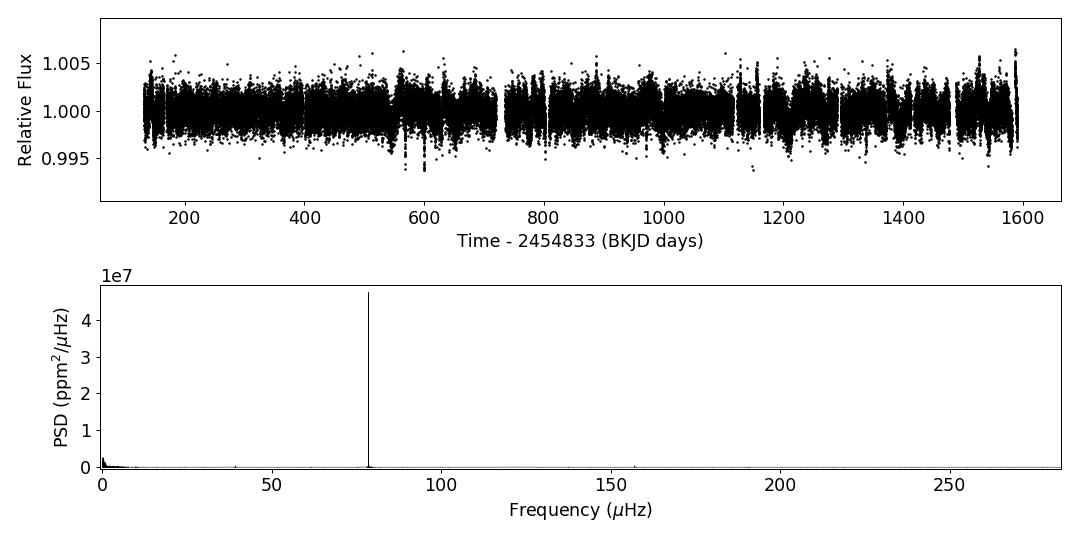
\includegraphics[width=0.9\linewidth]{Chapter5/2438148_lc_ps.png}
    \caption[Light curves and power spectra for KIC\,2572134 and KIC\,2438148]{Light curves and power spectra for KIC\,2572134 (top) and KIC\,2438148 (bottom).}
    \label{fig:weirdvars}
\end{figure}

\section{Ensemble Analysis}

\subsection{Extraction of global parameters}
We have identified 10 and 3 red giants in NGC\,6791 and NGC\,6819, respectively, for which we can now measure oscillation properties for the first time. We used the in-built estimation routines from the \texttt{Lightkurve} package to extract initial estimates of the global asteroseismic parameters, \numax{} and \dnu{}, from the corrected light curves. The \texttt{estimate\_numax} routine uses a 2D auto-correlation function (ACF) to estimate the value of \numax{} from a background corrected power spectrum. Whilst this package can be applied to most red giant oscillators, it is not designed to detect low-frequency oscillations, such as those in high-luminosity red giants. Furthermore, it provides no uncertainty measurement on the \numax{} or \dnu{} values.

To obtain uncertainties on our \numax{} values, we used the \texttt{exoplanet} Gaussian Process (GP) code \citep{foreman-mackey_fast_2017} to simultaneously model the granulation noise and red giant power excess for each light curve. This model relies on an implementation of a \texttt{Celerite} model for asteroseismic modelling with a dual kernel component for modelling stellar granulation, combined with a kernel centred around the \texttt{lightkurve} \numax{} estimate for the red giant power excess, and a constant white noise component. In a few cases, the low signal-to-noise of the excess required a third granulation component to be included for a good fit to be achieved. 

Figure \ref{fig:pm_model} shows an example of a fit of the asteroseismic model to the power excess of KIC\,2437653. The light curve and power spectrum are displayed in the first two panels. The initial fit (middle left) includes the log-scaled power spectrum overlaid with the individual components of the GP model and the complete initial power spectrum fit. The Hamiltonian Monte Carlo (HMC) sampled parameter distribution for the power excess and amplitude are shown (bottom left). We overlaid 100 randomly selected power spectral density trace samples on the original power spectrum (middle right) to highlight the distribution of the fit around \numax{}$\sim$75\,$\mu$\,Hz. Finally, we measured the uncertainty on our \numax{} parameter using a 94\% Highest Posterior Density (HPD) interval in the sampled distribution (bottom right) to account for skewed distributions.

\begin{figure}
    \centering
    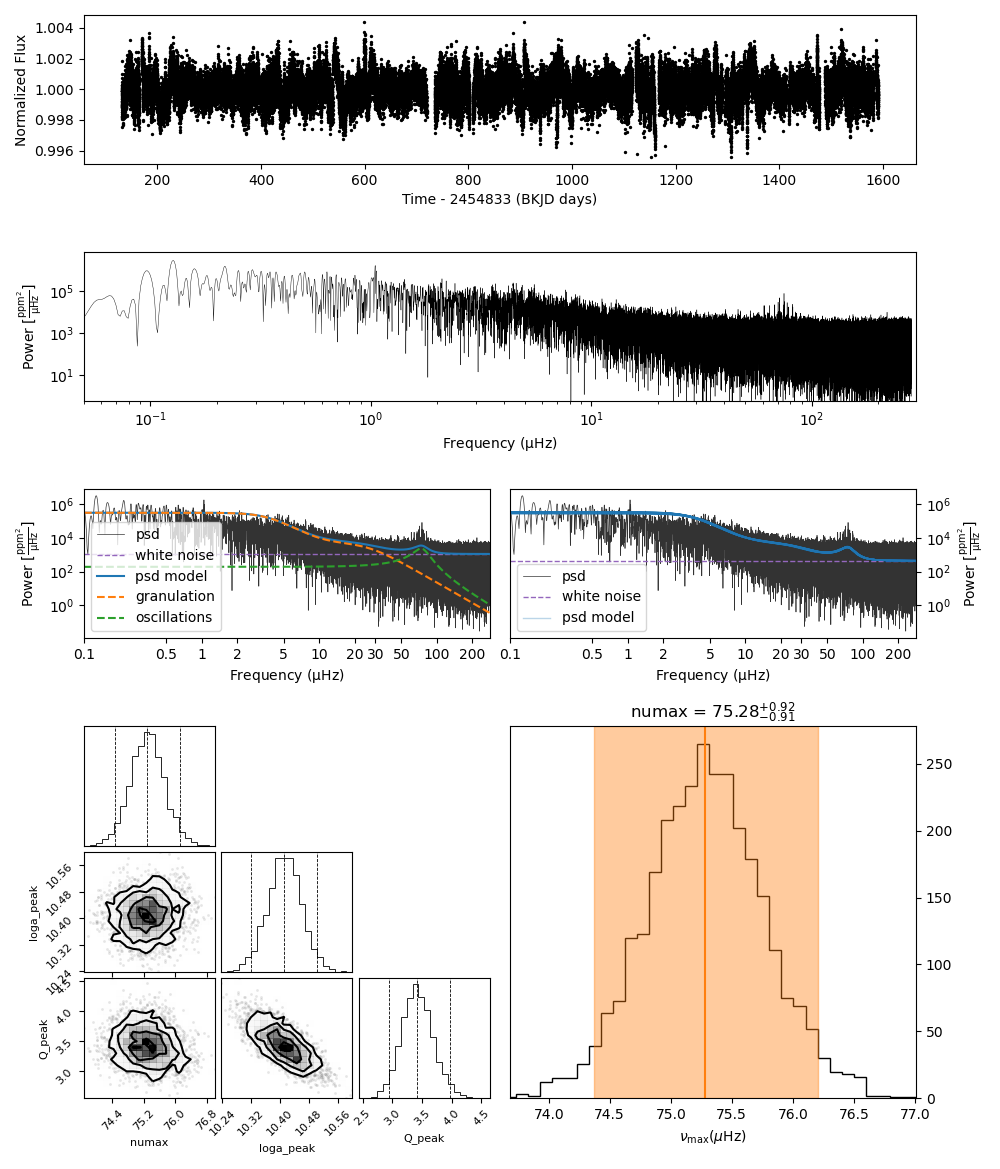
\includegraphics[width=0.95\textwidth]{Chapter5/2437653_pymc3_numax.png}
    \caption[Example of a fit by the asteroseismic GP model for KIC 2437653]{Example of a fit by the asteroseismic GP model for KIC\,2437653. The corrected light curve and resulting power spectrum used in this fit are shown (top two panels). The initial fit (top left) includes the log-scaled power spectrum overlaid with: the two component granulation background (yellow dashed line), the red giant oscillation power excess (green dashed line), white noise (purple dashed line) and the summed model (blue line). The Hamiltonian Monte Carlo (HMC) sampled parameter distribution for the power excess frequency, width, and amplitude, and their correlation, are shown (bottom left), with the distribution of the sampled \numax{} values expanded (bottom right) to highlight the mean value of 75.28\,$\mu$Hz (orange line) and the included uncertainties (orange shaded box). The evaluated power spectral densities for a selection of 100 trace parameter sets is overlaid in blue on the original power spectrum (middle right).}
    \label{fig:pm_model}
\end{figure}

%This has the added benefit of working in the time domain, ... Describe GPs here as well. Whilst this technique should be applicable to extracting deltanu and epsilon we were unable to get this working and have left this extension as future work. For now we have extracted numax for all RGBs with a much lower uncertainty on the extracted/sampled values than can be gained using the Sydney Pipeline. %Due to the memory-intensive nature of this work this was run using the Artemis HPC cluster.

We measured \dnu{} for each red giant by creating interactive \'echelle diagrams with the \texttt{\'Echelle} routine \citep{daniel_hey_echelle_2020}, and selecting the \dnu{} parameter so the $l = 0$ ridge appeared vertical. We then adjusted the value of \dnu{} until the ridge deviated noticeably from vertical and recorded this value as our uncertainty. Finally, we calculated the $\epsilon$ phase shift by measuring the position of the $l = 0$ mode ridge (see \cref{sect:ech}). Figures \ref{fig:echelle_new_6791} and \ref{fig:echelle_new2_6791} show the \'echelle diagrams of each new red giant in NGC\,6791 in which we detected oscillations. Figure~\ref{fig:echelle_new_6819} shows the same for NGC\,6819, with Figure~\ref{fig:echelle_new2_6819} showing \`echelles for red giants identified by \cite{bellamy_using_2015} and which we have created \`echelle diagrams for the first time whilst measuring the phase shift. We present our measured asteroseismic parameters for our newly-identified red giants in Table \ref{tab:6791rgc}, along with two stars we have identified as likely blends, and two stars we present as likely M-giant members, but whose resolution is too low for accurate mode identification to be achieved.

\begin{figure}
    \centering
        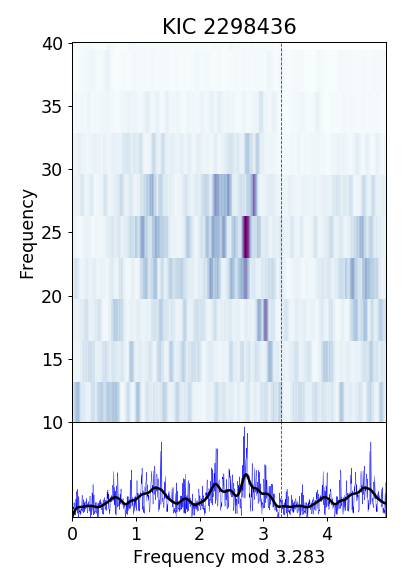
\includegraphics[width=0.3\textwidth]{Chapter5/2298436_echelle.png}
        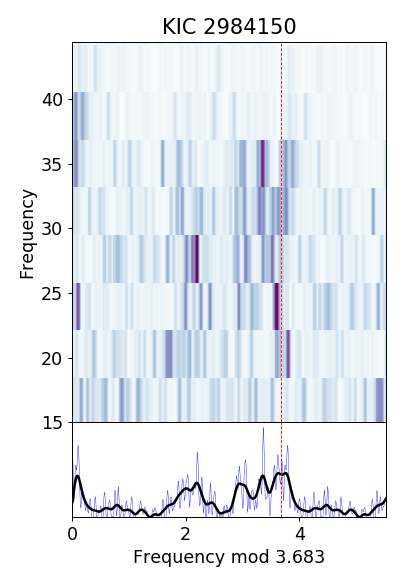
\includegraphics[width=0.3\textwidth]{Chapter5/2984150_echelle.png}
        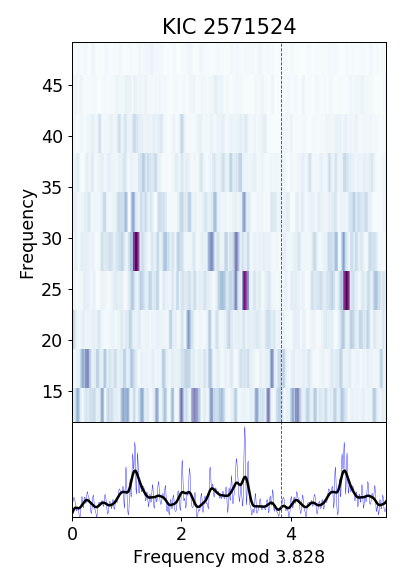
\includegraphics[width=0.3\textwidth]{Chapter5/2571524_echelle.png}
        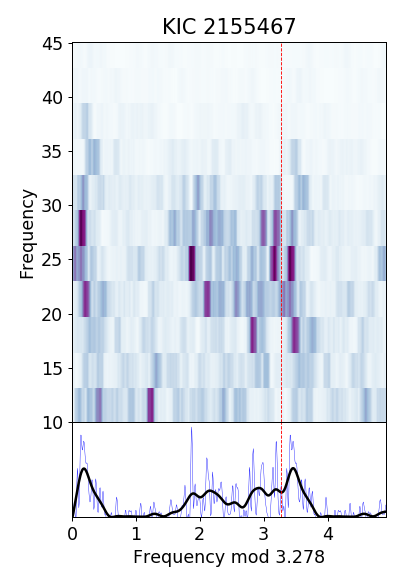
\includegraphics[width=0.3\textwidth]{Chapter5/2155467_echelle.png}
        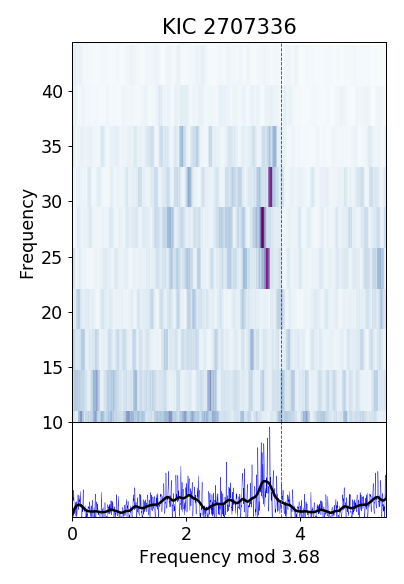
\includegraphics[width=0.3\textwidth]{Chapter5/2707336_echelle.png}
    \caption[\'Echelle diagrams for the newly identified cluster red giants in NGC\,6791 (I)]{\'Echelle diagrams for the newly identified NGC\,6791 red giants, ordered by \numax{}. The red line represents \dnu{} with the \'echelle extended to 1.5 \dnu{} to aid in identifying the $l = 0$ modes when $\epsilon$ is around 1.}
    \label{fig:echelle_new_6791}
\end{figure}

\begin{figure}
    \centering
        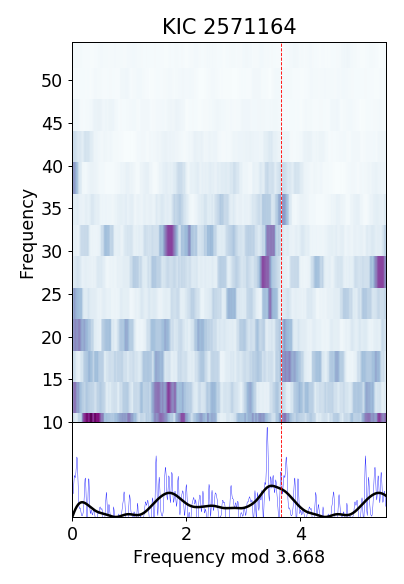
\includegraphics[width=0.3\textwidth]{Chapter5/2571164_echelle.png}
        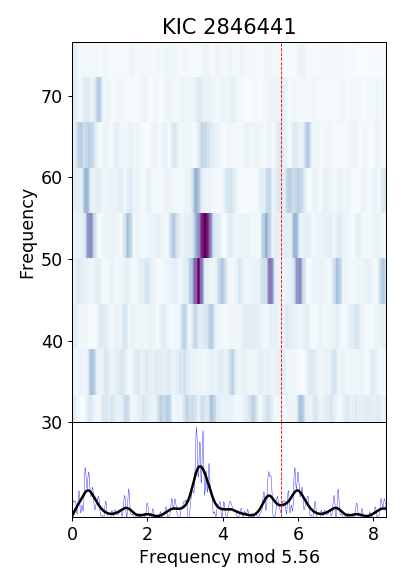
\includegraphics[width=0.3\textwidth]{Chapter5/2846441_echelle.png}
        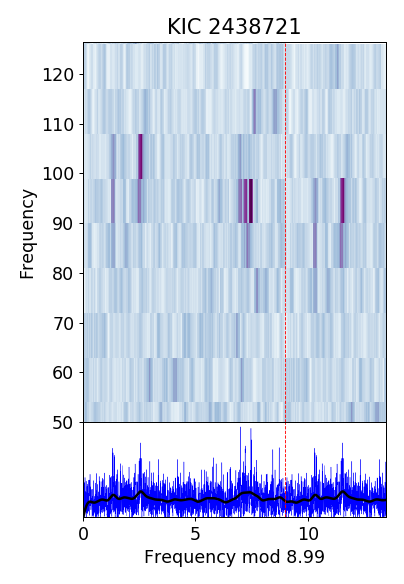
\includegraphics[width=0.3\textwidth]{Chapter5/2438721_echelle.png}
        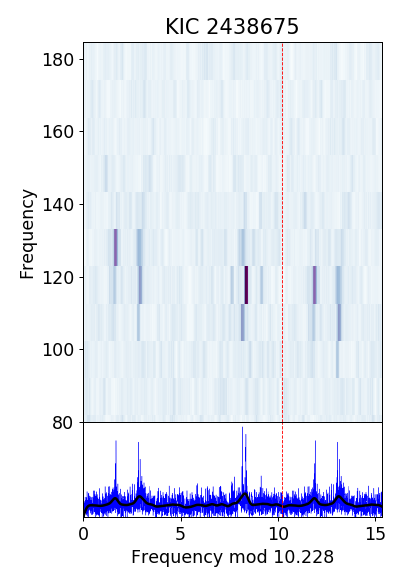
\includegraphics[width=0.3\textwidth]{Chapter5/2438675_echelle.png}
        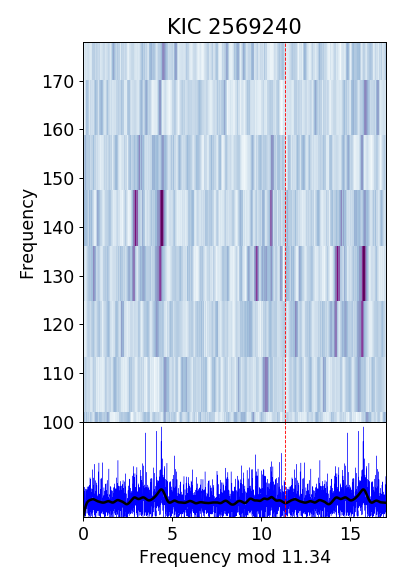
\includegraphics[width=0.3\textwidth]{Chapter5/2569240_echelle.png}
    \caption[\'Echelle diagrams for the newly identified cluster red giants in NGC\,6791 (II)]{Continued from Figure \ref{fig:echelle_new_6791}}
    \label{fig:echelle_new2_6791}
\end{figure}

\begin{figure}
    \centering
        % 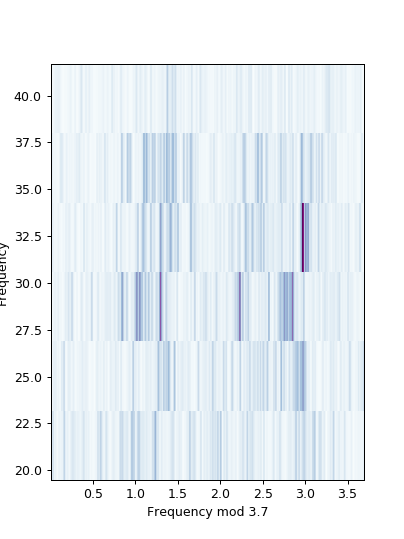
\includegraphics[width=0.32\textwidth]{Chapter5/2437817_echelle_new.png}
        % 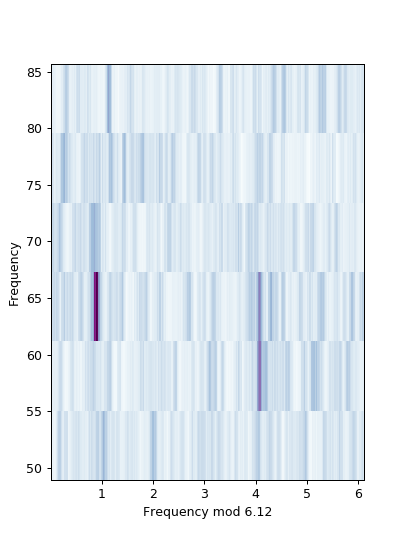
\includegraphics[width=0.32\textwidth]{Chapter5/2438053_echelle_new.png}
        \includegraphics[width=0.32\textwidth]{Chapter5/5024511_echelle.png}
        \includegraphics[width=0.32\textwidth]{Chapter5/5024571_echelle.png}
        \includegraphics[width=0.32\textwidth]{Chapter5/5200223_echelle.png}
        % \includegraphics[width=0.32\textwidth]{Chapter5/5025060_echelle_new.png}
    \caption[\'Echelle diagrams for the newly identified cluster red giants in NGC\,6819 (I)]{Same as Figure \ref{fig:echelle_new_6791} but for NGC\,6819.}
    \label{fig:echelle_new_6819}
\end{figure}

\begin{figure}
    \centering
    \includegraphics[width=0.32\textwidth]{Chapter5/5024582_echelle.png}
    \includegraphics[width=0.32\textwidth]{Chapter5/5112734_echelle.png}
    \includegraphics[width=0.32\textwidth]{Chapter5/5111718_echelle.png}
    \includegraphics[width=0.32\textwidth]{Chapter5/5024517_a_echelle.png}
    \includegraphics[width=0.32\textwidth]{Chapter5/5024517_b_echelle.png}
    
    \caption[\'Echelle diagrams for the identified cluster red giants in NGC\,6819 (II)]{Same as Figure \ref{fig:echelle_new_6819} for stars identified in Beau Bellamy's thesis \citep{bellamy_using_2015}, that we have produced \`echelle diagrams for, for the first time. The last two panels show individual \`echelle diagrams for the two red giant power excesses we have identified in KIC\,5024517.}
    \label{fig:echelle_new2_6819}
\end{figure}

\begin{table}
    \centering
    \setlength\tabcolsep{10pt}
    \resizebox{\textwidth}{!}{%
        \begin{tabular}{cccccccccccccccccl}
            \toprule
            KIC ID	&	NGC		&  meanprob	&K$_\mathrm{p}$ &	\numax{}	&	GP $\nu_{\mathrm{max}}$	&	\dnu{}	&	$\sigma_{\Delta\nu}$	&	$\epsilon$	&	Notes	\\
            \midrule
            2847282 &   6791    &   0.721   &   8.34        &   0.68        &         \textemdash       &\textemdash&   \textemdash     &  \textemdash& New M-giant \\
            2155467	&	6791	&	0.899	&	14.08		&	30.14		&  26.78$^{+0.63}_{-0.61}$  &	3.28	&		0.05		&	1.06	&	\\
            2298436	&	6791	&	0.903	&	14.02		&	28.87		&  26.07$^{+0.45}_{-0.39}$ &	3.28	&		0.07		&	0.84	&	\\
            2438675	&	6791	&	0.950	&	15.47		&	117.9		&         \textemdash       &	10.23	&		0.03		&	1.28	&	\\
            2438721	&	6791	&	0.789	&	15.75		&	97.26		&112.29$^{+27.52}_{-26.57}$	&	8.99	&		0.03		&	1.28	&	\\
            2569240	&	6791	&	0.964	&	15.71		&	137.46		&         \textemdash       &	11.34	&		0.08		&	1.39	&	\\
            2571164	&	6791	&	0.896	&	14.20		&	34.88		&  32.39$^{+1.05}_{-1.13}$	&	3.67	&		0.10	    &	0.95	&	\\
            2571524	&	6791	&	0.744	&	14.25		&	29.69		&  31.50$^{+0.98}_{-0.90}$  &	3.83	&		0.10		&	0.83	&	\\
            2707336	&	6791	&	0.924	&	14.30		&	33.55		&  31.31$^{+0.64}_{-0.61}$  &	3.68	&		0.10	    &	0.93	&	\\
            2846441	&	6791	&	0.744	&	14.41		&	56.81		&  54.17$^{+1.67}_{-1.89}$  &	5.56	&		0.20	    &	1.08	&	\\
            2984150	&	6791	&	0.620	&	14.19		&	29.32		&  31.35$^{+0.78}_{-0.71}$  &	3.68	&		0.10	    &	1.02	&	\\
            \midrule
            2437817	&	6791	&	0.967	&	16.54		&	32.19		&         \textemdash       &	3.7		&		0.20		&	0.80	&	Likely blend with KIC\,2437805\\
            2438053	&	6791	&	0.964	&	16.49		&	58.93		&         \textemdash       &	6.13	&		0.02		&	0.66	&	Likely blend with KIC\,2438038\\
            \midrule
            5024511	&	6819	&	0.147	&	12.31		&	24.43		&  31.65$^{+0.64}_{-0.88}$  &	2.66	&		0.20		&	0.95	&	RG light curve has contamination from $\delta$ Scuti\\
            5024571	&	6819	&	0.773	&	14.28		&	39.13		&         \textemdash       &	4.12	&		0.10	    &	0.99	&	RG light curve has contamination from $\delta$ Scuti\\
            5200223	&	6819	&	0.294	&	14.19		&	3.77		&						    &	0.71	&		0.05		&	0.72	&	\\
            \midrule
            5024582	&	6819	&	0.304	&	10.30		&	46.44		&         \textemdash       &	4.72	&		0.10		&	1.07	&	New \dnu{} and $\epsilon$ measurements\\
            5112734	&	6819	&	0.961	&	10.20		&	41.19		&         \textemdash       &	4.12	&		0.10		&	1.04	&	New \dnu{} and $\epsilon$ measurements\\
            5111718	&	6819	&	0.818	&	11.48		&	134.2		&         \textemdash       &	10.47	&		0.20		&	1.33	&	New \dnu{} and $\epsilon$ measurements\\
        5024517 (A)	&	6819	&	0.960	&	9.62		&	23.35		&         \textemdash       &	4.88	&		0.10		&	1.02	&	New \dnu{} and $\epsilon$ measurements\\
        5024517 (B)	&	6819	&	0.960	&	9.62		&	50.72		&         \textemdash       &	2.65	&		0.10		&	1.00	&	New \dnu{} and $\epsilon$ measurements\\
            5112751	&	6819	&	0.915	&	10.34		&	84.73		&         \textemdash       &	6.18	&		0.10		&	1.03	&	New \dnu{} and $\epsilon$ measurements\\
            \midrule
            5112483	&	6819	&	0.433	&	11.24		&\textemdash	&         \textemdash       &\textemdash&   \textemdash	&\textemdash	&	Likely M-Giant from LC. Resolution too low for order matching.\\
            5200056	&	6819	&	0.639	&	10.88		&\textemdash	&         \textemdash       &\textemdash&   \textemdash	&\textemdash	&	Likely M-Giant from LC. Resolution too low for order matching.\\

            \bottomrule
        \end{tabular}
    }
    \caption[List of newly identified red giants]{List of newly identified red giants from this work. GP \numax{} values are not available for KIC\,2438675 and KIC\,2569240 as the signal-to-noise of the red giant excess was too low to obtain a constrained fit, while in KIC\,5024571, the contaminating $\delta$ Scuti oscillations prevented the GP model from converging. GP \numax{} values were not calculated for the RGs identified by Beau Bellamy in his Masters' thesis \citep{bellamy_using_2015}, these are included to present our new $\epsilon$ and \dnu{} measurements only.}
    \label{tab:6791rgc}
\end{table}

\section{Asteroseismic Diagrams}

For large ensemble asteroseismic analyses, we must reduce stellar spectra to a few measurable parameters that describe fundamental stellar properties. These parameters for solar-like oscillators include \numax{}, \dnu{}, and $\epsilon$. Asteroseismic diagrams provide an intuitive format for investigating the relationships between these parameters and their corresponding connection to the intrinsic stellar properties. In the case of open clusters, where populations are considered to be coeval and co-metallic, we have ideal ensembles for investigating stellar evolutionary tracks and thus the function of stellar mass in these diagrams. These functions can then be applied to larger samples where age or metallicity may be unknown. We present cluster red giants on the same \numax{} \textendash{} \dnu{} and \dnu{} \textendash{} $\epsilon$ diagrams as the entire \Kepler{} sample for the first time, effectively presenting empirical isochrones based on the homogeneous cluster properties. Hereafter, we refer to these empirical isochrones showing tight relationships in \numax{}, $\Delta\nu$, $\epsilon$, and photometric magnitudes as isochrones.

We combined the red giant samples from \cite{hon_deep_2018}, \cite{yu_asteroseismology_2018-1} and \cite{yu_asteroseismology_2020}, as well as red giants from Beau Bellamy's Masters' thesis \citep{bellamy_using_2015}, to produce a complete sample of previously studied red giants in the nominal \Kepler{} FoV, henceforth referred to as the field star sample. We then cross-matched this sample with our likely red giant cluster membership lists to isolate the studied cluster red giants for NGC\,6791 and NGC\,6819. We note that \numax{} and \dnu{} for all of the red giants in \cite{hon_deep_2018} have also been extracted by either \cite{yu_asteroseismology_2018-1} or \cite{yu_asteroseismology_2020}. Yu et al.'s combined sample (Yu) is slightly larger than that of \cite{hon_deep_2018} for the cluster red giants, so we selected their values for these parameters for consistency. By combining the results from Yu, and Bellamy, with our new detections, we obtained determinations for \numax{} and \dnu{} for 150 and 131 stars in NGC\,6791 and NGC\,6819, respectively.

\cite{stello_asteroseismic_2011} have shown that cluster red giants show a tight relationship between apparent magnitude and their asteroseismic parameters of \numax{} and \dnu{}. This is a result of the similar masses and effective temperatures shared by red giant cluster members. The luminosity differences between cluster members is therefore the dominant factor affecting these values, which corresponds to apparent magnitude for cluster members because they are effectively co-distant. \cite{stello_detection_2010} and \cite{bellamy_new_2015} have shown that this relationship can be used for asteroseismic cluster membership determinations. Figure \ref{fig:magdnu} shows the $K$ mag vs \dnu{} relation for the clusters of NGC\,6791 and NGC\,6819. The cluster members of single isolated stars are clearly delineated into isochrones, with the red clumps visible just above the RGB sequences around \numax{}$\sim$30\,$\mu$Hz and $\Delta\nu\sim$3.8$\mu$Hz. 

We identified 46 and 21 outliers for the NGC\,6791 and NGC\,6819 ensembles, respectively, which were classified in Beau Bellamy's thesis as likely members. We reclassify these stars as likely non-members based on this diagram although a small fraction could be exotic stars arising from interactions with other stars. Our membership analysis does not account for binary systems, making a numerical estimate of the likelihood of membership for these stars difficult, although future Gaia releases should have the ability to distinguish binary stars based on astrometric excess noise \citep{gandhi_astrometric_2020}. This will provide future analyses with the option of dividing the dataset into multiple stellar systems and single star systems prior to clustering, allowing us to identify and account for kinematic deviations from the average cluster values, arising from the motion of binaries. The possibility of even a small fraction of these stars being members with exotic interaction histories makes these interesting targets for follow up investigations. 

We also note the presence of 2 potential evolved blue stragglers in NGC\,6791, lying about 0.75\,mag above the isochrone in the $K$ mag \textendash \dnu{} diagram. We categorise these stars as potential evolved BSs as they both have high membership scores, so are very likely cluster members, and have magnitudes with an offset of 0.75\,mag from the empirical cluster isochrone, corresponding to the maximum offset expected from a binary merger between 2 equal mass stars. Binary merger products often appear on or near the main sequence, to the blue of the cluster's main-sequence turnoff point. Such stars are called blue stragglers and as these stars evolve off the main sequence they remain blue of the red giant branch, where they are referred to as evolved blue stragglers. KIC\,5025717 also lies within this same magnitude range of the empirical cluster isochrone for NGC\,6819. Whilst it falls outside the \Kepler{} superstamps it was targeted in the nominal mission, and all three stars exhibit red giant power excesses \citep{yu_asteroseismology_2016}. Figure \ref{fig:ebss} presents PDCSAP-based amplitude spectra we have extracted from these nominal \Kepler{} targets. It is possible other evolved blue stragglers could also be present in this sample with smaller magnitude offsets from non-equal mass mergers, although such an investigation is beyond the scope of the current work.

\begin{figure}
    \centering
    \includegraphics[width=\linewidth]{Chapter5/kmag-dnu-both.png}
    % \includegraphics[width=0.48\linewidth]{Chapter5/stello_11_kmagdnu.png}
    \caption[$K$mag \textendash \dnu{} relation for NGC\,6791 and NGC\,6819]{$K$mag \textendash \dnu{} relation for NGC\,6791 (red) and NGC\,6819 (blue), with outliers (grey) from our compiled database (left) and the corresponding diagram from \citep{stello_asteroseismic_2011} (right). Outliers (grey) may include exotic cluster members such as mergers.}
    \label{fig:magdnu}
\end{figure}

\begin{figure}
    \centering
    \includegraphics[width=0.95\linewidth]{Chapter5/ebss_ps.png}
    \caption[Amplitude spectra of three potential evolved blue straggler stars]{Amplitude spectra of the three potential evolved blue straggler stars we have identified in NGC\,6791 and NGC\,6819 showing solar-like oscillations.}
    \label{fig:ebss}
\end{figure}


\subsubsection{\numax{} \textendash \dnu{} relation}

\cite{hekker_characteristics_2009} first showed the tight correlation between \dnu{} and \numax{} for red giants using \textsc{CoRoT} data. This relation has since been further investigated \cite[eg.][]{stello_relation_2009, huber_testing_2011}, with \cite{yu_asteroseismology_2018-1} conducting the most detailed investigation to date, using over 16,000 red giants. \cite{ hekker_asteroseismic_2011} first produced this plot for the cluster ensembles of NGC\,6791 and NGC\,6819, including 46 and 42 red giant members, respectively. Figure \ref{fig:nike_6791} presents an updated view of this diagram (top panel) with 150 and 131 red giant members for NGC\,6791 and NGC\,6819, respectively, more than doubling the number of cluster members in each case. The grey points in this figure present the field star sample (Yc) for comparison. 

\cite{yu_asteroseismology_2018-1} showed a modified version of this plot, with \numax{}$^{0.75}$/\dnu{} plotted on the ordinate axis. This new axis removes the diagonal trend and highlighted the trend of increasing mass with increasing ordinate value. This trend enables us to use the ordinate axis as a proxy for stellar mass. We produced similar plots for each cluster (bottom panel), and note that clear isochrones for each cluster are superimposed on the field distribution. The red giants in NGC\,6819 form a horizontal population, and reveal a near constant mass, whilst the red clump and evolved red giant stars appear as an excess within the \numax{} range of $\sim25$\textendash{}$35\,\mu$Hz for NGC\,6791 and $\sim40$\textendash{}$50\,\mu$Hz for NGC\,6819. In both clusters, but particularly in NGC\,6791 this excess lies slightly below a linear fit to the stars outside this \numax{} range. Since the ordinate axis is a proxy for mass, this confirms the clear mass-loss measured by \cite{miglio_asteroseismology_2012} in NGC\,6791, with a more complete sample of the cluster red giants, and hints at a negligible mass-loss within NGC\,6819 red clump stars. In addition, we have provided a comparison to the distribution of field red giants for the first time.

\begin{figure}
    \centering
    \includegraphics[width=\linewidth]{Chapter5/numax_dnu_both_2.png}
    \includegraphics[width=\linewidth]{Chapter5/numax_dnusc_both_2.png}
    \caption[\numax{} \textendash \dnu{} diagram for NGC\,6791 and NGC\, 6819]{\numax{} \textendash \dnu{} diagram for NGC\,6791 (top) and NGC\,6819 (bottom). The ensemble from \cite{yu_asteroseismology_2018-1} (grey) are overlaid with the cluster members (Chapter \ref{chap:membership}) from \cite{yu_asteroseismology_2018-1} and \cite{yu_asteroseismology_2020} (green), \cite{bellamy_using_2015} (blue) and those we have newly extracted values for from this work (red). }
    \label{fig:nike_6791}
\end{figure}

\subsubsection{$\epsilon$ \textendash $\Delta\nu$ Diagram}

\cite{huber_asteroseismology_2010} and \cite{mosser_mixed_2011} showed that \dnu{} is also highly correlated with the phase term, $\epsilon$, for red giants. \cite{corsaro_asteroseismology_2012} plotted this relation for the cluster ensembles and presented fits for:

\begin{equation}
    \epsilon = A + B \mathrm{log}\Delta\nu
\end{equation}

\noindent in agreement with those found by \cite{mosser_universal_2011} for \textsc{CoRoT} red giants and \cite{kallinger_evolutionary_2012} for $\sim$900 \Kepler{} red giants with 600\,days of data. We have recreated this diagram for the complete sample of \Kepler{} red giant field stars, overlaid with our complete ensemble of cluster members in Figure \ref{fig:eps_6791}. Yc did not measure $\epsilon$ values for the cluster red giants so we have constructed the field distribution with values quoted by \cite{hon_deep_2018}, which were reproduced from \cite{stello_suppression_2016}.  This is the first time the ensemble of cluster red giants has been overlaid on the field distribution, and clear isochrones are apparent for each cluster, tracing lines of almost constant mass. The red clump distributions form distinct groups for each cluster, with slightly lower $\epsilon$ values than the red giants with similar \dnu{} values. This is consistent with the cluster isochrones shown by \cite{corsaro_asteroseismology_2012}.

\begin{figure}
    \centering
    \includegraphics[height=0.5\textheight]{Chapter5/epsilon_combined.png}
    \caption[$\epsilon$ \textendash \dnu{} diagram for NGC\, 6791 and NGC\, 6819 cluster members]{$\epsilon$ \textendash \dnu{} diagram for NGC\,6791 (red) and NGC\,6819 (blue) cluster members with values from \cite{hon_search_2019} (circles) and this work (squares) overlaid on the red giant field distribution}
    \label{fig:eps_6791}
\end{figure}

\section{Conclusions}

In this chapter, we have presented a complete sample of cluster red giants for NGC\,6791 and NGC\,6819, to the limit of red giant oscillation detections. We have re-classified some stars that we found to be likely astrometric members to be non-members based on their photometric variability. This allowed us to produce an improved cluster membership determination compared to our membership in Chapter \ref{chap:membership}. We have also shown clear isochrones exist for each cluster in both the \numax{} - \dnu{} and $\epsilon$ - \dnu{} relations, and have produced updated asteroseismic diagrams for the cluster red giant ensembles, with the field distribution included for the first time for comparison with these isochrones.



% \section{Seismic Membership}

% Following \cite{stello_asteroseismic_2011} and \cite{bellamy_new_2015} we calculated global \numax{} and \dnu{} parameters for each star based on the scaling relations, and assuming the distance modulus, average red giant mass, and metallicity of the clusters shown in \cref{tab:cluster_params}.

% \begin{figure}
%     \centering
%     \includegraphics[width=0.48\linewidth]{Chapter5/numax_pred.png}
%     \includegraphics[width=0.48\linewidth]{Chapter5/deltanu_pred.png}
%     \caption{Caption}
%     \label{fig:predicted_seismic}
% \end{figure}

% \begin{table}[h]
%     \centering
%     \begin{tabular}{c|cc|cc}
%             & \multicolumn{2}{c}{{\bf NGC\,6791}} & \multicolumn{2}{c}{{\bf NGC\,6819}}   \\
%         & {\bf Value}   & {\bf Reference}           & {\bf Value}  & {\bf Reference}              \\
%         $m-M_0$     & 13.09   & \cite{wu_asteroseismic_2014}      & 11.747 & \cite{abedigamba_distance_2016}\\
%         RG Mass     & 1.23    & \cite{miglio_asteroseismology_2012}  & 1.61   & \cite{miglio_asteroseismology_2012}\\
%         Metallicity & 0.34    &                     & 0.09   &                        \\
%     \end{tabular}
%     \caption{Global cluster parameters used to calculate the asteroseismic global parameters for each red giant based on the scaling relations.}
%     \label{tab:cluster_params}
% \end{table}

% \begin{figure}
%     \centering
%     \includegraphics[height=1.75\linewidth]{Chapter5/teff_comp.png}
%     \caption{Caption}
%     \label{fig:teff}
% \end{figure}



%Teff calculation and comparison.


% \section{Asteroseismology}

% \section{Solar-like Oscillators}
% \subsection{Red giants}

% \subsection{Subgiants}

% \section{Eclipsing binaries}

% \section{RR Lyrae oscillators}
% \newpage
% \section{Acknowledgements}

% The author would like to thank Daniel Hey, as well as supervisors Tim Bedding and Dennis Stello for many helpful discussions, direction and suggestions that have enabled this chapter. Daniel Hey developed the echelle routine and provided helpful discussions and debugging suggestions for the initial Pymc3/exoplanet routine that evolved into the one used here to extract numax.
%The author acknowledges the Sydney Informatics Hub and the University of Sydney’s high performance computing cluster, Artemis, for providing the computing resources that have contributed to the results reported herein. % Work on cluster RGs - orientation
\chapter{Conclusions and Future Work}

I conclude that when my thesis is completed life will be better... % Work on cluster RGs - mode identification/modelling
\input{Chapter_Future} % Future work to be completed
\input{Chapter_Summary/Summary} % Summary & Conclusions

% \cleardoublepage
% \renewcommand{\thepage}{\rm \arabic{page}}
% \setcounter{page}{1}
% %\renewcommand\chapterheadstartvskip{\vspace*{-5\baselineskip}}

%\cleardoublepage
%\input{chapter2/ch2}
%\cleardoublepage
%\input{chapter3/ch3}
%\cleardoublepage
%\input{chapter4/ch4}
%\cleardoublepage
%\input{chapter5/conclusions}
%\cleardoublepage
%\input{chapter6/gamaGroups}
%\cleardoublepage
%\input{chapter7/futureWork}
%\cleardoublepage
%\input{chapterLast/end}
%\cleardoublepage
% \input{backmatter/}
% \bibliographystyle{apalike}
\bibliographystyle{mn2e}`
\bibliography{bibi}
\end{document}
